\chapter{NESTOR}
The Neumann Solver for Toroidal Regions~(NESTOR) provides the free-boundary contribution to the energy functional in VMEC~\cite{merkel_1986, hirshman_vanrij_merkel_1986}.

\FloatBarrier
\section{Problem statement}
The basic geometry is depicted in Fig.~\ref{fig:00_regions}.
\begin{figure}[htbp]
  \centering
  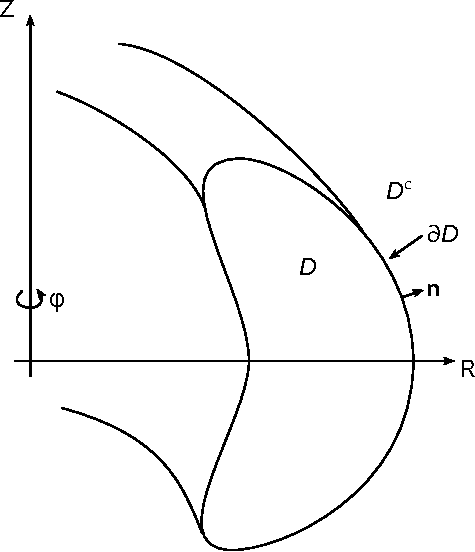
\includegraphics[width=0.3\textwidth]{img/00_regions.pdf}
  \caption{The interior region $\mathcal{D}$ (for the plasma) and the exterior region $\mathcal{D}^\mathrm{c}$ (for the coils) are separated by the boundary $\partial\mathcal{D}$.
           The outward-directed (exterior) unit normal vector is denoted $\mathbf{n}$.}
  \label{fig:00_regions}
\end{figure}

The magnetic field in this situation is denoted $\mathbf{B}_0$.
It is generated by currents $\mathbf{j}$ in $\mathcal{D} \cup \mathcal{D}^\mathrm{c}$:
\begin{equation}
  \nabla \times \mathbf{B}_0 = \mu_0 \mathbf{j}, ~ \nabla \cdot \mathbf{B}_0 = 0 \, .
\end{equation}
A magnetic scalar potential $\Phi$ can be found,
such that the corresponding magnetic field $\mathbf{B} = \nabla \Phi$ cancels the normal component of $\mathbf{B}_0$ on $\partial\mathcal{D}$:
\begin{equation}
  \left( \mathbf{B}_0 + \nabla \Phi \right) \cdot \mathbf{n} = 0 \, .
\end{equation}
The magnetic scalar potential $\Phi$ solves Laplace's equation
with the given Neumann boundary condition:
\begin{align}
  \forall \mathbf{x} \in \mathcal{D}:         &~ \Delta \Phi(\mathbf{x}) = 0 \, , \label{eqn:laplacePhi} \\
  \forall \mathbf{x} \in \partial\mathcal{D}: &~ \frac{\partial \Phi(\mathbf{x})}{\partial \mathbf{n}} = - \mathbf{B}_0(\mathbf{x}) \cdot \mathbf{n} \, . \label{eqn:bnorm}
\end{align}
Green's second identity for on-surface evaluations~(\ref{eqn:GreensIdentityOnSurface}) is used
to convert Laplace's equation for~$\Phi$ in \eqn{laplacePhi} into an integral equation:
\begin{equation}
  \forall \mathbf{x} \in \partial \mathcal{D}: ~
  \Phi(\mathbf{x}) + \frac{1}{2 \pi} \int\limits_{\partial\mathcal{D}} \frac{\partial G(\mathbf{x},\mathbf{x}')}{\partial \mathbf{n}'}                \Phi(\mathbf{x}')                        \mathrm{d}S'
                   = \frac{1}{2 \pi} \int\limits_{\partial\mathcal{D}}                G(\mathbf{x},\mathbf{x}')                        \frac{\partial \Phi(\mathbf{x}')}{\partial \mathbf{n}'} \mathrm{d}S' \, .
  \label{eqn:laplaceIntegral}
\end{equation}
The right hand side of \eqn{laplaceIntegral} is given by the normal component of the magnetic field (see \eqn{bnorm})
and acts as a source term here. The outward-directed unit normal vector at location~$\mathbf{x}'$ is denoted~$\mathbf{n}'$
and $G(\mathbf{x},\mathbf{x}')$ is Green's function as in \eqn{GreensFunction}.

\FloatBarrier
\section{Parity of the Magnetic Scalar Potential}
Let $\mathbf{B}_0$ be the total magnetic field on the plasma boundary of a stellarator.
Using the NESTOR~\cite{merkel_1986} code, a scalar magnetic potential~$\Phi$ can be determined
such that the corresponding solenoidal magnetic field~$\mathbf{B} = \nabla \Phi$
cancels the normal component of the total magnetic field on the boundary:
\begin{equation}
  \left(\mathbf{B}_0 + \nabla \Phi \right) \cdot \mathbf{n} = 0 \, ,
\end{equation}
where $\mathbf{n}$ is the surface normal vector.
The current density representing the coils and the plasma is assumed to be stellarator-symmetric,
which implies that the total magnetic field~$\mathbf{B}_0$ must be stellarator-symmetric as well~\cite{dewar_hudson_1998_stellarator_symmetry}.
Thus, it is concluded that the magnetic scalar potential~$\Phi$ and the solenoidal magnetic field~$\mathbf{B}$ derived from
it are stellarator-symmetric as well.

This note adresses the partity of the magnetic scalar potential
in order to reason whether to use $\sin(m\theta-n\zeta)$~(odd parity) or $\cos(m\theta-n\zeta)$~(even parity) Fourier basis functions for the stellarator-symmetric part of $\Phi$.

The magnetic field is expressed in cylindrical components:
\begin{equation}
  \mathbf{B} = \mathbf{B}(\rho, \varphi, z) = \left[ B_\rho, B_\varphi, B_z \right] \, .
\end{equation}
The relation of $\mathbf{B}$ to the scalar magnetic potential~$\Phi$ is as follows:
\begin{equation}
    \mathbf{B} = \nabla \Phi
  =                  \frac{\partial \Phi}{\partial \rho}    \hat{\mathbf{e}}_\rho
    + \frac{1}{\rho} \frac{\partial \Phi}{\partial \varphi} \hat{\mathbf{e}}_\varphi
    +                \frac{\partial \Phi}{\partial z}       \hat{\mathbf{e}}_z \, . \label{eqn:comp_B}
\end{equation}
Stellarator symmetry of $\mathbf{B}$ implies the following relation for the components of $\mathbf{B}$
under the symmetry operation $I_0$:
\begin{equation}
  I_0 \left[ B_\rho, B_\varphi, B_z \right] = \left[ -B_\rho, B_\varphi, B_z \right] \, . \label{eqn:vec_symm}
\end{equation}
Regarding derivatives, the following holds for an arbitrary scalar function $f$ and in particular for the scalar magnetic potential $\Phi$~\cite{dewar_hudson_1998_stellarator_symmetry}:
\begin{equation}
        \left[ \frac{\partial}{\partial \rho},   \frac{\partial}{\partial \varphi},   \frac{\partial}{\partial z} \right] I_0 f
  = I_0 \left[ \frac{\partial}{\partial \rho}, - \frac{\partial}{\partial \varphi}, - \frac{\partial}{\partial z} \right]     f \, . \label{eqn:der_symm}
\end{equation}
The symmetry operation $I_0$ is applied to $\mathbf{B}$ and Eqn.~(\ref{eqn:der_symm}) is applied (note that $I_0 \rho = \rho$):
\begin{align}
    I_0 \mathbf{B}
  =& I_0 \left( \nabla \Phi \right)
  =  I_0 \left[ \frac{\partial \Phi}{\partial \rho}, \frac{1}{\rho} \frac{\partial \Phi}{\partial \varphi}, \frac{\partial \Phi}{\partial z} \right]
  =  \left[ \frac{\partial}{\partial \rho}, - \frac{1}{\rho}\frac{\partial}{\partial \varphi}, - \frac{\partial}{\partial z} \right] I_0 \Phi \nonumber \\
  =& \left[ \frac{\partial}{\partial \rho} \left( I_0 \Phi \right), - \frac{1}{\rho}\frac{\partial}{\partial \varphi} \left( I_0 \Phi \right), - \frac{\partial}{\partial z} \left( I_0 \Phi \right) \right] \nonumber \\
  =& \left[ - \frac{\partial}{\partial \rho} \left(- I_0 \Phi \right), \frac{1}{\rho}\frac{\partial}{\partial \varphi} \left(- I_0 \Phi \right), \frac{\partial}{\partial z} \left(- I_0 \Phi \right) \right] \, .
\end{align}
Component-wise comparison with Eqn.~(\ref{eqn:comp_B}) and use of the symmetry property~(\ref{eqn:vec_symm}) leads to:
\begin{align}
  B_\rho    =& \frac{\partial \Phi}{\partial \rho} = -I_0 B_\rho = \frac{\partial}{\partial \rho} \left( -I_0 \Phi \right) \Rightarrow \Phi = -I_0 \Phi \Leftrightarrow I_0 \Phi = - \Phi \\
  B_\varphi =& \frac{1}{\rho}\frac{\partial \Phi}{\partial \varphi} = I_0 B_\varphi = \frac{1}{\rho} \frac{\partial}{\partial \varphi} \left(- I_0 \Phi \right) \Rightarrow I_0 \Phi = - \Phi \\
  B_z       =& \frac{\partial \Phi}{\partial z} = I_0 B_z = \frac{\partial}{\partial z} \left( -I_0 \Phi \right) \Rightarrow I_0 \Phi = - \Phi \, .
\end{align}
Concluding, $I_0 \Phi = - \Phi$ is consistent with $\mathbf{B}$ being stellarator-symmetric when $\mathbf{B} = \nabla \Phi$
and this implies that $\Phi$ has \underline{odd} parity and can thus be represented using only a $\sin(m\theta-n\zeta)$ Fourier basis.

\FloatBarrier
\section{Analytical formulation}

\FloatBarrier
\subsection{Coordinate System}
The toroidal surface $\partial\mathcal{D}$ is doubly periodic.
It is thus natural to introduce normalized angle-like coordinates
$0\leq u \leq 1$ and $0 \leq v \leq 1$ for the poloidal and toroidal directions, respectively.
The cylindrical coordinates $(r,\varphi,z)$ on the surface $\partial\mathcal{D}$ are then parameterized with two-dimensional Fourier series as follows:
\begin{align}
  r(u,v)     =& \sum\limits_{m=-m_\mathrm{b}}^{m_\mathrm{b}} \sum\limits_{n=-n_\mathrm{b}}^{n_\mathrm{b}}
    \hat{r}_{m,n} \exp\left( 2 \pi i (m u + n v) \right) \, , \,  \hat{r}_{m,n}^* = \hat{r}_{-m,-n} \, , \nonumber \\
  z(u,v)     =& \sum\limits_{m=-m_\mathrm{b}}^{m_\mathrm{b}} \sum\limits_{n=-n_\mathrm{b}}^{n_\mathrm{b}}
    \hat{z}_{m,n} \exp\left( 2 \pi i (m u + n v) \right) \, , \,  \hat{z}_{m,n}^* = \hat{z}_{-m,-n} \, , \\
  \varphi(v) =& \frac{2 \pi}{n_\mathrm{p}} v \, . \nonumber
\end{align}
The cartesian coordinates of points on the surface in a module~$l$ of a $n_\mathrm{p}$-fold toroidally symmetric
configuration, e.g., a stellarator, then read:
\begin{equation}
  \mathbf{x}^{(l)}(u,v) =
    \begin{pmatrix}
      r(u,v) \cdot \cos\left( \frac{2 \pi}{n_\mathrm{p}} (l-1+v) \right) \\
      r(u,v) \cdot \sin\left( \frac{2 \pi}{n_\mathrm{p}} (l-1+v) \right) \\
      z(u,v)
    \end{pmatrix} ,
    \, l = 1, ..., n_\mathrm{p}
    \label{eqn:def_x}
\end{equation}
and the tangential derivatives are denoted $\mathbf{x}_u \equiv \partial \mathbf{x}/\partial u$ and $\mathbf{x}_v \equiv \partial \mathbf{x}/\partial v$
and a shorthand notation is introduced for the first toroidal period as $\mathbf{x} = \mathbf{x}^{(1)}$.
The notation $\mathbf{x}' = \mathbf{x}(u',v')$ with the definition of $\mathbf{x}$ from \eqn{def_x} is used
and leads to
\begin{equation}
  \mathbf{x}'_{u'} = \frac{\partial \mathbf{x}'(u',v')}{\partial u'} = \left. \frac{\partial \mathbf{x}}{\partial u} \right\rvert_{\substack{u=u'\\v=v'}}
  \, \mathrm{and} ~~
  \mathbf{x}'_{v'} = \frac{\partial \mathbf{x}'(u',v')}{\partial v'} = \left. \frac{\partial \mathbf{x}}{\partial v} \right\rvert_{\substack{u=u'\\v=v'}} \, .
\end{equation}

A change of variables is now performed in \eqn{laplaceIntegral} to the normalized coordinates $u$ and $v$.
The Jacobian of the transformation is (according to Eqn.~(2.5.48a) in Ref.~\cite{dHaseleer}):
\begin{equation}
  \mathrm{d}S' = |\mathbf{x}'_{u'} \times \mathbf{x}'_{v'}| \,\mathrm{d}u' \,\mathrm{d}v' \, . \label{eqn:surfaceJacobian}
\end{equation}
The normal vector $\mathbf{n}'$ can be expressed in terms of the tangential derivatives (after Eqn.~(2.3) in Ref.~\cite{merkel_1987}):
\begin{equation}
  \mathbf{n}' = \frac{\mathbf{x}'_{u'} \times \mathbf{x}'_{v'}}{|\mathbf{x}'_{u'} \times \mathbf{x}'_{v'}|} \, . \label{eqn:normalVector}
\end{equation}
The normal derivative of Green's function is:
\begin{equation}
    \frac{\partial G(\mathbf{x},\mathbf{x}')}{\partial \mathbf{n}'}
  = \nabla G(\mathbf{x},\mathbf{x}') \cdot \mathbf{n}'
  = \frac{\mathbf{x}-\mathbf{x}'}{|\mathbf{x}-\mathbf{x}'|^3} \cdot \frac{\mathbf{x}'_{u'} \times \mathbf{x}'_{v'}}{|\mathbf{x}'_{u'} \times \mathbf{x}'_{v'}|} \, . \label{eqn:normalGreensFunction}
\end{equation}

\FloatBarrier
\subsection{Formulation of Laplace's Equation}
Inserting \eqn{normalVector} into \eqn{bnorm} and this as well as \eqn{surfaceJacobian} and~(\ref{eqn:normalGreensFunction}) into \eqn{laplaceIntegral}, one obtains:
\begin{equation}
  \forall (u,v) \in [0,1]^2: ~
    \Phi(u,v)
  + \int\limits_0^1 \int\limits_0^1
      g(u,v,u',v')
      \Phi(u', v')
      \,\mathrm{d}u' \,\mathrm{d}v'
  = \int\limits_0^1 \int\limits_0^1
      h(u,v,u',v')
      \,\mathrm{d}u' \,\mathrm{d}v' \, .
  \label{eqn:laplaceIntegralUV}
\end{equation}
with
\begin{align}
    g(u,v,u',v')
  =& \, \frac{1}{2 \pi}
    \sum\limits_{l=1}^{n_\mathrm{p}}
    \frac{\mathbf{x}-\mathbf{x}'^{(l)}}{|\mathbf{x}-\mathbf{x}'^{(l)}|^3} \cdot \frac{\mathbf{x}'^{(l)}_{u'} \times \mathbf{x}'^{(l)}_{v'}}{ \bcancel{|\mathbf{x}'^{(l)}_{u'} \times \mathbf{x}'^{(l)}_{v'}|} }
    \bcancel{|\mathbf{x}'^{(l)}_{u'} \times \mathbf{x}'^{(l)}_{v'}|} \nonumber \\
  =& \, \frac{1}{2 \pi}
    \sum\limits_{l=1}^{n_\mathrm{p}}
    \frac{ \left( \mathbf{x}-\mathbf{x}'^{(l)} \right) \cdot \left( \mathbf{x}'^{(l)}_{u'} \times \mathbf{x}'^{(l)}_{v'} \right) }{|\mathbf{x}-\mathbf{x}'^{(l)}|^3} \label{eqn:def_g}
\end{align}
and
\begin{align}
    h(u,v,u',v')
  =& \frac{1}{2 \pi}
    \sum\limits_{l=1}^{n_\mathrm{p}} \frac{1}{|\mathbf{x}-\mathbf{x}'^{(l)}|}
    \left( - \mathbf{B}_0(\mathbf{x}') \cdot \frac{\mathbf{x}'^{(l)}_{u'} \times \mathbf{x}'^{(l)}_{v'}}{ \bcancel{|\mathbf{x}'^{(l)}_{u'} \times \mathbf{x}'^{(l)}_{v'}|} } \right)
    \bcancel{|\mathbf{x}'^{(l)}_{u'} \times \mathbf{x}'^{(l)}_{v'}|} \nonumber \\
  =&\frac{1}{2 \pi}
    \sum\limits_{l=1}^{n_\mathrm{p}}
    \frac{ - \mathbf{B}_0(\mathbf{x}') \cdot \left( \mathbf{x}'^{(l)}_{u'} \times \mathbf{x}'^{(l)}_{v'} \right) }{|\mathbf{x}-\mathbf{x}'^{(l)}|} \, . \label{eqn:def_h}
\end{align}

\FloatBarrier
\subsection{Transformation to Fourier Space}
The magnetic scalar potential $\Phi$ is a doubly-periodic function in $u$ and $v$ and can be represented as a Fourier series:
\begin{equation}
    \Phi(u,v)
  = \sum\limits_{m=-\infty}^{+\infty} \sum\limits_{n=-\infty}^{+\infty}
    \hat{\Phi}_{m,n} e^{2 \pi i (m u + n v)} \label{eqn:fourierPhi}
\end{equation}
with
\begin{equation}
 \hat{\Phi}^*_{m,n}=\hat{\Phi}_{-m,-n} \, .
\end{equation}
This representation of $\Phi(u,v)$ is now inserted into \eqn{laplaceIntegralUV}
and it holds for all $(u,v)$:
\begin{align}
  ~& \sum\limits_{m,n}
    \hat{\Phi}_{m,n} e^{2 \pi i (m u + n v)}
  + \int\limits_0^1 \int\limits_0^1
      g(u,v,u',v')
      \left(\sum\limits_{m',n'} \hat{\Phi}_{m',n'} e^{2 \pi i (m' u' + n' v')} \right)
      \,\mathrm{d}u' \,\mathrm{d}v' \nonumber \\
  =& \int\limits_0^1 \int\limits_0^1
      h(u,v,u',v')
      \,\mathrm{d}u' \,\mathrm{d}v' \, .
\end{align}
The summation over $m', n'$ and the corresponding Fourier coefficients $\hat{\Phi}_{m',n'}$ can be pulled outside of the integral:
\begin{align}
  ~& \sum\limits_{m,n}
    \hat{\Phi}_{m,n} e^{2 \pi i (m u + n v)}
  + \sum\limits_{m',n'}
    \left(
      \int\limits_0^1 \int\limits_0^1
        g(u,v,u',v') e^{2 \pi i (m' u' + n' v')}
      \,\mathrm{d}u' \,\mathrm{d}v' \right)
    \hat{\Phi}_{m',n'} \nonumber \\
 =& \int\limits_0^1 \int\limits_0^1
      h(u,v,u',v')
      \,\mathrm{d}u' \,\mathrm{d}v' \, . \label{eqn:laplace_only_Phi_Fourier}
\end{align}
The two integrals appearing here can be considered as functions of $u$ and $v$
and are expressed as Fourier series as well:
\begin{align}
  \hat{g}_{m',n'}(u, v)
  \equiv&\, \int\limits_0^1 \int\limits_0^1
         g(u,v,u',v') e^{2 \pi i (m' u' + n' v')}
         \,\mathrm{d}u' \,\mathrm{d}v' \nonumber \\
  =&\, \sum\limits_{m,n} \hat{g}_{m,n,m',n'} e^{2 \pi i (m u + n v)} \label{eqn:fourier_g}
\end{align}
with
\begin{align}
     \hat{g}_{m,n,m',n'}
  \equiv&\, \int\limits_0^1 \int\limits_0^1
         \hat{g}_{m',n'}(u, v)
         e^{-2 \pi i(m u + n v)}
       \,\mathrm{d}u \,\mathrm{d}v \nonumber \\
  =& \int\limits_0^1 \int\limits_0^1
       \left(
         \int\limits_0^1 \int\limits_0^1
           g(u,v,u',v') e^{2 \pi i (m' u' + n' v')}
           \,\mathrm{d}u' \,\mathrm{d}v'
       \right)
       e^{-2 \pi i(m u + n v)}
       \,\mathrm{d}u \,\mathrm{d}v
\end{align}
as well as
\begin{align}
  \tilde{h}(u,v)
  \equiv&\, \int\limits_0^1 \int\limits_0^1
         h(u,v,u',v')
         \,\mathrm{d}u' \,\mathrm{d}v' \nonumber \\
  =&\, \sum\limits_{m,n} \hat{h}_{m,n} e^{2 \pi i (m u + n v)} \label{eqn:fourier_h}
\end{align}
with
\begin{align}
     \hat{h}_{m,n}
  \equiv&\, \int\limits_0^1 \int\limits_0^1
         \tilde{h}(u,v)
         e^{-2 \pi i(m u + n v)}
       \,\mathrm{d}u \,\mathrm{d}v \nonumber \\
  =& \int\limits_0^1 \int\limits_0^1
       \left(
         \int\limits_0^1 \int\limits_0^1
           h(u,v,u',v')
           \,\mathrm{d}u' \,\mathrm{d}v'
       \right)
       e^{-2 \pi i(m u + n v)}
       \,\mathrm{d}u \,\mathrm{d}v \, .
\end{align}
These Fourier integrals can be reordered a little bit, leading to:
\begin{align}
     \hat{g}_{m,n,m',n'}
  =& \int\limits_0^1 \int\limits_0^1
     \int\limits_0^1 \int\limits_0^1
       g(u,v,u',v')
       e^{2 \pi i (m' u' + n' v' - m u - n v)}
       \,\mathrm{d}u \,\mathrm{d}v
       \,\mathrm{d}u' \,\mathrm{d}v' \label{eqn:ft_g} \\
     \hat{h}_{m,n}
  =& \int\limits_0^1 \int\limits_0^1
     \int\limits_0^1 \int\limits_0^1
       h(u,v,u',v')
       e^{-2 \pi i(m u + n v)}
       \,\mathrm{d}u \,\mathrm{d}v
       \,\mathrm{d}u' \,\mathrm{d}v' \label{eqn:ft_h} \, .
\end{align}
The Fourier representations of the integrals over $g$ and $h$ from \eqn{fourier_g} and \eqn{fourier_h}
can be inserted back into Laplace's equation~(\ref{eqn:laplace_only_Phi_Fourier}):
\begin{equation}
    \sum\limits_{m,n}
    \hat{\Phi}_{m,n} e^{2 \pi i (m u + n v)}
  + \sum\limits_{m',n'}
    \left( \sum\limits_{m,n} \hat{g}_{m,n,m',n'} e^{2 \pi i (m u + n v)} \right)
    \hat{\Phi}_{m',n'}
  = \sum\limits_{m,n} \hat{h}_{m,n} e^{2 \pi i (m u + n v)} \, .
\end{equation}
The summations in the middle of above equation can be swapped:
\begin{equation}
    \sum\limits_{m,n}
      \hat{\Phi}_{m,n}
    e^{2 \pi i (m u + n v)}
  + \sum\limits_{m,n}
      \sum\limits_{m',n'}
      \hat{g}_{m,n,m',n'}
      \hat{\Phi}_{m',n'}
    e^{2 \pi i (m u + n v)}
  = \sum\limits_{m,n}
      \hat{h}_{m,n}
    e^{2 \pi i (m u + n v)} \, .
\end{equation}
This equation holds for all $(u,v) \in [0,1]^2$.
The orthogonality of the Fourier basis therefore allows to consider only the Fourier coefficients.
This leads to the following infinite set of linear equations:
\begin{align}
  \forall\, (m,n) \in [-\infty,+\infty]^2 :& \,
    \hat{\Phi}_{m,n}
  + \sum\limits_{m'=-\infty}^{+\infty} \sum\limits_{n'=-\infty}^{+\infty}
      \hat{g}_{m,n,m',n'} \hat{\Phi}_{m',n'}
  = \hat{h}_{m,n} \\
  \Leftrightarrow
  \forall\, (m,n) \in [-\infty,+\infty]^2 :& \,
  \sum\limits_{m'=-\infty}^{+\infty} \sum\limits_{n'=-\infty}^{+\infty}
    \left( \hat{g}_{m,n,m',n'} + \delta_{m,m'} \delta_{n,n'} \right) \hat{\Phi}_{m',n'}
  = \hat{h}_{m,n} \label{eqn:linsys_inf} \, .
\end{align}
%
A matrix~$\mathbf{A}$ and a right-hand side~$\mathbf{b}$
can be defined:
\begin{align}
 (\mathbf{A})_{m,n,m',n'} =&\, \hat{g}_{m,n,m',n'} + \delta_{m,m'} \delta_{n,n'} \\
 (\mathbf{b})_{m,n}       =&\, \hat{h}_{m,n}
\end{align}
as well as a solution vector~$\mathbf{x}$:
\begin{equation}
 (\mathbf{x})_{m',n'} = \hat{\Phi}_{m',n'}
\end{equation}
in order to cast \eqn{linsys_inf} into a linear system of equations:
\begin{equation}
 \mathbf{A} \mathbf{x} = \mathbf{b} \, .
\end{equation}
The Fourier resolution is truncated at some maximum Fourier mode numbers $M$, $N$
in order to arrive at a finite-dimensional linear system of equations,
which then can be solved by standard linear algebra methods,
e.g., from \texttt{LAPACK}.

The remainder of this chapter
deals with the computation of the matrix elements
$\hat{g}_{m,n,m',n'}$ and $\hat{h}_{m,n}$
as well as the computation of the vacuum magnetic pressure
from the obtained solution vector $\hat{\Phi}_{m',n'}$.

\FloatBarrier
\subsection{Cancellation of Singularities using a Subtraction Method}
The kernel functions $g$ and $h$ are singular if simultaneously $u=u'$ and $v=v'$.
Their Fourier transforms in \eqn{ft_g} and \eqn{ft_h} thus cannot be evaluated directly
using standard discrete Fourier transform methods.
The trick is now to subtract a function with the same singular behaviour as the function to be transformed
which can be analytically Fourier-transformed.
%
A Taylor expansion of $|\mathbf{x}-\mathbf{x}'|$ around fixed values of $(u',v')$ is considered.
\begin{equation}
  |\mathbf{x}-\mathbf{x}'| = \sqrt{ (\mathbf{x}-\mathbf{x}') \cdot (\mathbf{x}-\mathbf{x}') } \, . \label{eqn:dist_x_xprime}
\end{equation}
First look at $\mathbf{x}-\mathbf{x}'$:
\begin{align}
  \mathbf{x}-\mathbf{x}'
     =   &    \underbrace{ \left. (\mathbf{x}-\mathbf{x}') \right\rvert_{\substack{u=u'\\v=v'}} }_{
               \begin{aligned}=&\, \mathbf{x}'-\mathbf{x}' \\=&\, 0 \end{aligned} }
           + \underbrace{ \left. \frac{\partial(\mathbf{x}-\mathbf{x}')}{\partial u} \right\rvert_{\substack{u=u'\\v=v'}} }_{
               \begin{aligned}= \underbrace{\left. \frac{\partial \mathbf{x} }{\partial u}\right\rvert_{\substack{u=u'\\v=v'}}}_{=\mathbf{x}'_{u'}}
                              - \underbrace{\left. \frac{\partial \mathbf{x}'}{\partial u}\right\rvert_{\substack{u=u'\\v=v'}}}_{= 0} \end{aligned}} (u-u')
           + \underbrace{ \left. \frac{\partial(\mathbf{x}-\mathbf{x}')}{\partial v} \right\rvert_{\substack{u=u'\\v=v'}} }_{
               \begin{aligned}= \underbrace{\left. \frac{\partial \mathbf{x} }{\partial v}\right\rvert_{\substack{u=u'\\v=v'}}}_{=\mathbf{x}'_{v'}}
                              - \underbrace{\left. \frac{\partial \mathbf{x}'}{\partial v}\right\rvert_{\substack{u=u'\\v=v'}}}_{= 0} \end{aligned}} (v-v') \nonumber \\
    ~ &\,+ \frac{1}{2} \left[ \mathbf{x}'_{u' u'} (u-u')^2 + 2\, \mathbf{x}'_{u' v'} (u-u') (v-v') + \mathbf{x}'_{v' v'} (v-v')^2 \right] + \, ... \nonumber \\
  \approx&\, \phantom{+}~\underbrace{\mathbf{x}'_{u'} (u-u') + \mathbf{x}'_{v'} (v-v')}_{\textrm{first-order contribution}} \label{eqn:dist_1stOrder} \\
     ~   &\,          +  \underbrace{\frac{1}{2} \left[ \mathbf{x}'_{u' u'} (u-u')^2 + 2\, \mathbf{x}'_{u' v'} (u-u') (v-v') + \mathbf{x}'_{v' v'} (v-v')^2 \right]}_{\textrm{second-order contribution}} \label{eqn:dist_2ndOrder}
\end{align}
due to neglection of higher-order terms.
Inserting the first-order approximation from \eqn{dist_1stOrder} into \eqn{dist_x_xprime} leads to:
\begin{align}
  |\mathbf{x}-\mathbf{x}'|
  \approx &\, \sqrt{ \left[ \mathbf{x}'_{u'} (u-u') + \mathbf{x}'_{v'} (v-v') \right]^2 } \nonumber \\
      =   &\, \sqrt{ {\mathbf{x}'}^2_{u'} (u-u')^2 + 2 \mathbf{x}'_{u'} \mathbf{x}'_{v'} (u-u') (v-v') + {\mathbf{x}'}^2_{v'} (v-v')^2 } \, . \label{eqn:approx_dist}
\end{align}
Only the contribution to $h$ from the toroidal period in which $\mathbf{x}$ is located is singular.
This is equivalent to only considering the first period ($l=1$), since the numbering of toroidal periods is arbitrary.
The approximation from \eqn{approx_dist} is inserted
into the contribution from the first toroidal period to $h$ from \eqn{def_h}:
\begin{equation}
  h(u-u',v-v',u',v')
  \approx\, \frac{1}{2 \pi}
  \frac{- \mathbf{B}_0(\mathbf{x}') \cdot \left( \mathbf{x}'_{u'} \times \mathbf{x}'_{v'} \right)}
       {\left( {\mathbf{x}'}^2_{u'} (u-u')^2 + 2 \mathbf{x}'_{u'} \mathbf{x}'_{v'} (u-u') (v-v') + {\mathbf{x}'}^2_{v'} (v-v')^2 \right)^{1/2}} \, . \label{eqn:approx_h}
\end{equation}
Similarly, only the contribution to $g$ from the first toroidal period ($l=1$) is singular.
The first- and second-order contributions of $\mathbf{x}-\mathbf{x}'$ from \eqn{dist_1stOrder} and \eqn{dist_2ndOrder}
and the first-order approximation of $|\mathbf{x}-\mathbf{x}'|$ from \eqn{approx_dist}
are inserted into the contribution from the first toroidal period to $g$ in \eqn{def_g}:
\begin{align}
  ~ &\, 2 \pi g(u,v,u',v') \nonumber \\
  \approx &\, \phantom{+}~\frac{  \left[ \mathbf{x}'_{u'} (u-u') + \mathbf{x}'_{v'} (v-v') \right] \cdot \left( \mathbf{x}'_{u'} \times \mathbf{x}'_{v'} \right)}
                               {  \left[ {\mathbf{x}'}^2_{u'} (u-u')^2 + 2 \mathbf{x}'_{u'} \mathbf{x}'_{v'} (u-u') (v-v') + {\mathbf{x}'}^2_{v'} (v-v')^2 \right]^{3/2}} \label{eqn:g_1stOrder} \\
     ~    &\,          +  \frac{  \left[ \mathbf{x}'_{u' u'} (u-u')^2 + 2\, \mathbf{x}'_{u' v'} (u-u') (v-v') + \mathbf{x}'_{v' v'} (v-v')^2 \right] \cdot \left( \mathbf{x}'_{u'} \times \mathbf{x}'_{v'} \right)}
                               {2 \left[ {\mathbf{x}'}^2_{u'} (u-u')^2 + 2 \mathbf{x}'_{u'} \mathbf{x}'_{v'} (u-u') (v-v') + {\mathbf{x}'}^2_{v'} (v-v')^2 \right]^{3/2}} \label{eqn:g_2ndOrder}
\end{align}
Note that the first-order contribution from \eqn{g_1stOrder} to the approximation of $g$ vanishes, since
\begin{align*}
  \mathbf{x}'_{u'} \cdot& \left( \mathbf{x}'_{u'} \times \mathbf{x}'_{v'} \right) = 0 ~ \mathrm{and}\\
  \mathbf{x}'_{v'} \cdot& \left( \mathbf{x}'_{u'} \times \mathbf{x}'_{v'} \right) = 0 \, .
\end{align*}
Therefore, the approximation of $g$ can be reduced to:
\begin{equation}
  g(u-u',v-v',u',v') \approx \frac{1}{2 \pi}
    \frac{A (u-u')^2 + 2 B (u-u') (v-v') + C (v-v')^2}
         {\left[ {\mathbf{x}'}^2_{u'} (u-u')^2 + 2 \mathbf{x}'_{u'} \mathbf{x}'_{v'} (u-u') (v-v') + {\mathbf{x}'}^2_{v'} (v-v')^2 \right]^{3/2}}
  \label{eqn:approx_g}
\end{equation}
with
\begin{align}
  A \equiv& \frac{1}{2} \mathbf{x}'_{u' u'} \cdot \left( \mathbf{x}'_{u'} \times \mathbf{x}'_{v'} \right) \, , \nonumber \\
  B \equiv& \frac{1}{2} \mathbf{x}'_{u' v'} \cdot \left( \mathbf{x}'_{u'} \times \mathbf{x}'_{v'} \right) ~ \mathrm{and} \label{eqn:def_ABC}\\
  C \equiv& \frac{1}{2} \mathbf{x}'_{v' v'} \cdot \left( \mathbf{x}'_{u'} \times \mathbf{x}'_{v'} \right) \, . \nonumber
\end{align}
The derivatives with respect to normalized coordinates are transformed into derivatives
with respect to the actual coordinates by application of the chain rule:
\begin{align}
  A =& \frac{1}{2} \frac{\partial^2 \mathbf{x}'}{\partial {u'}^2} \cdot \mathbf{N}'
    =  \frac{1}{2} \underbrace{ \left( \frac{\partial \theta'}{\partial u'} \right)^2}_{=(2\pi)^2} \frac{\partial^2 \mathbf{x}'}{\partial {\theta'}^2} \cdot \mathbf{N}'
    =  (2\pi)^2 \underbrace{\left( \frac{1}{2} \frac{\partial^2 \mathbf{x}'}{\partial {\theta'}^2} \cdot \mathbf{N}' \right)}_{\equiv a_{u,u}} \\
 2B =& \bcancel{2} \frac{1}{\bcancel{2}} \frac{\partial^2 \mathbf{x}'}{\partial u' \partial v'} \cdot \mathbf{N}'
    =  \underbrace{ \frac{\partial \theta'}{\partial u'} \frac{\partial \zeta'}{\partial v'} }_{=(2\pi)^2}
       \underbrace{ \frac{\partial \phi'}{\partial \zeta'} }_{=1/n_\mathrm{fp}}
       \frac{\partial^2 \mathbf{x}'}{\partial \theta' \partial \phi'} \cdot \mathbf{N}'
    =  (2\pi)^2 \underbrace{\left(\frac{1}{n_\mathrm{fp}} \frac{\partial^2 \mathbf{x}'}{\partial \theta' \partial \phi'} \cdot \mathbf{N}' \right)}_{\equiv a_{u,v}} \\
  C =& \frac{1}{2} \frac{\partial^2 \mathbf{x}'}{\partial {v'}^2} \cdot \mathbf{N}'
    =  \frac{1}{2}
       \underbrace{ \left( \frac{\partial \zeta'}{\partial v'} \right)^2}_{=(2\pi)^2}
       \underbrace{ \left( \frac{\partial \phi'}{\partial \zeta'}\right)^2 }_{=1/n_\mathrm{fp}^2}\frac{\partial^2 \mathbf{x}'}{\partial {\phi'}^2} \cdot \mathbf{N}'
    =  (2\pi)^2 \underbrace{\left( \frac{1}{2} \frac{1}{n_\mathrm{fp}^2} \frac{\partial^2 \mathbf{x}'}{\partial {\phi'}^2} \cdot \mathbf{N}' \right)}_{\equiv a_{v,v}}
\end{align}
The components of the surface normal vector are given in \eqn{surfNComponents}
and the second derivatives of the surface geometry are given in \eqn{d2Xdt2}, \eqn{d2Xdtz} and \eqn{d2Xdz2}.
The terms $a_{u,u}$, $a_{u,v}$ and $a_{v,v}$ thus can be evaluated in cylindrical components:
\begin{align}
  a_{u,u} =& \frac{1}{2}
               \left(  \frac{\partial^2 R'}{\partial {\theta'}^2} {N^R}'
                     + \frac{\partial^2 Z'}{\partial {\theta'}^2} {N^Z}' \right) \label{eqn:auu} \\
  a_{u,v} =& \frac{1}{n_\mathrm{fp}}
               \left(  \frac{\partial^2 R'}{\partial \theta' \partial \phi'} {N^R}'
                     + \frac{\partial   R'}{\partial \theta'               } {N^\phi}'
                     + \frac{\partial^2 Z'}{\partial \theta' \partial \phi'} {N^Z}'      \right) \label{eqn:auv} \\
  a_{v,v} =& \frac{1}{2} \frac{1}{n_\mathrm{fp}^2}
               \left[  \left( \frac{\partial^2 R'}{\partial {\phi'}^2} - R' \right) {N^R}'
                     + 2      \frac{\partial   R'}{\partial \phi'  }                {N^\phi}'
                     +        \frac{\partial^2 Z'}{\partial {\phi'}^2}              {N^Z}'    \right] \label{eqn:avv} \, .
\end{align}
Shorthand notations are also introduced for the (squared and mixed) tangential derivatives:
\begin{align}
  a \equiv&\, {\mathbf{x}'}^2_{u'} \nonumber \\
  b \equiv&\,  \mathbf{x}'_{u'} \mathbf{x}'_{v'} \label{eqn:def_abc} \\
  c \equiv&\, {\mathbf{x}'}^2_{v'} \nonumber \, .
\end{align}
It follows:
\begin{align}
  a =&       \Biggl( \frac{\partial \mathbf{x}'}{\partial \theta'} \underbrace{\frac{\partial \theta'}{\partial u'}}_{=2\pi} \Biggr)
       \cdot \Biggl( \frac{\partial \mathbf{x}'}{\partial \theta'} \underbrace{\frac{\partial \theta'}{\partial u'}}_{=2\pi} \Biggr)
    =  (2 \pi)^2 \underbrace{\left( \frac{\partial \mathbf{x}'}{\partial \theta'} \cdot \frac{\partial \mathbf{x}'}{\partial \theta'} \right)}_{=g_{u,u}^\mathrm{b}} \\
 2b =& 2     \Biggl( \frac{\partial \mathbf{x}'}{\partial \theta'} \underbrace{\frac{\partial \theta'}{\partial u'}}_{=2\pi} \Biggr)
       \cdot \Biggl( \frac{\partial \mathbf{x}'}{\partial \phi'} \underbrace{\frac{\partial \phi'}{\partial \zeta'}}_{=1/n_\mathrm{fp}} \underbrace{\frac{\partial \zeta'}{\partial v'}}_{=2\pi} \Biggr)
    =  (2 \pi)^2 \underbrace{\left(\frac{2}{n_\mathrm{fp}} \frac{\partial \mathbf{x}'}{\partial \theta'} \cdot \frac{\partial \mathbf{x}'}{\partial \phi'} \right)}_{=g_{u,v}^\mathrm{b}} \\
  c =&       \Biggl( \frac{\partial \mathbf{x}'}{\partial \phi'} \underbrace{\frac{\partial \phi'}{\partial \zeta'}}_{=1/n_\mathrm{fp}} \underbrace{\frac{\partial \zeta'}{\partial v'}}_{=2\pi} \Biggr)
       \cdot \Biggl( \frac{\partial \mathbf{x}'}{\partial \phi'} \underbrace{\frac{\partial \phi'}{\partial \zeta'}}_{=1/n_\mathrm{fp}} \underbrace{\frac{\partial \zeta'}{\partial v'}}_{=2\pi} \Biggr)
    =  (2 \pi)^2 \underbrace{\left(\frac{1}{n_\mathrm{fp}^2} \frac{\partial \mathbf{x}'}{\partial \phi'} \cdot \frac{\partial \mathbf{x}'}{\partial \phi'} \right)}_{=g_{v,v}^\mathrm{b}} \, .
\end{align}
The cylindrical components of the first-order derivatives can be gotten from \eqn{dXdt} and \eqn{dXdp} and it follows:
\begin{align}
  g_{u,u}^\mathrm{b} =&       \left( \frac{\partial R'}{\partial \theta'}, 0, \frac{\partial Z'}{\partial \theta'} \right)
                        \cdot \left( \frac{\partial R'}{\partial \theta'}, 0, \frac{\partial Z'}{\partial \theta'} \right)
                     =  \left(\frac{\partial R'}{\partial \theta'} \right)^2 + \left( \frac{\partial Z'}{\partial \theta'} \right)^2 \label{eqn:guu_b} \\
  g_{u,v}^\mathrm{b} =& \frac{2}{n_\mathrm{fp}}
                              \left( \frac{\partial R'}{\partial \theta'}, 0 , \frac{\partial Z'}{\partial \theta'} \right)
                        \cdot \left( \frac{\partial R'}{\partial \phi'  }, R', \frac{\partial Z'}{\partial \phi'  } \right)
                     = \frac{2}{n_\mathrm{fp}} \left(  \frac{\partial R'}{\partial \theta'} \frac{\partial R'}{\partial \phi'}
                                                     + \frac{\partial Z'}{\partial \theta'} \frac{\partial Z'}{\partial \phi'} \right) \label{eqn:guv_b} \\
  g_{v,v}^\mathrm{b} =& \frac{1}{n_\mathrm{fp}^2} \left( \frac{\partial R'}{\partial \phi'}, R', \frac{\partial Z'}{\partial \phi'} \right)
                        \cdot                     \left( \frac{\partial R'}{\partial \phi'}, R', \frac{\partial Z'}{\partial \phi'} \right)
                     =  \frac{1}{n_\mathrm{fp}^2} \left[  \left( \frac{\partial R'}{\partial \phi'} \right)^2
                                                        + {R'}^2
                                                        + \left( \frac{\partial Z'}{\partial \phi'} \right)^2 \right] \label{eqn:gvv_b} \, .
\end{align}
The inhomogenity due to the normal component of the external magnetic field is denoted as
\begin{align}
  F(u',v') =&\, - \mathbf{B}_0(\mathbf{x}') \cdot \left( \mathbf{x}'_{u'} \times \mathbf{x}'_{v'} \right) \, .
\end{align}
The only dependance of \eqn{approx_h} on $u$ and $v$ is now in the terms $(u-u')$ and $(v-v')$.
In order to find a periodic approximation of $h$, it is thus required to find a periodic approximation of $(u-u')$ and $(v-v')$.
The normalized variables $u$ and $v$ are periodic over the interval $[0, 1]$ and thus $(u-u')$ spans the range $[-1, 1]$
for all possible combinations of $u$ and $u'$.
Consider the Taylor expansion of $\tan(x)$:
\begin{align}
              \tan(    x) =&\,     x \underbrace{+ \frac{1}{3} x^3 + \, ...}_{\mathrm{neglected}} \nonumber \\
  \Rightarrow \tan(\pi x) \approx &\,          \pi           x  \nonumber \\
  \Leftrightarrow      x  \approx &\, \frac{1}{\pi} \tan(\pi x) \nonumber \\
  \Rightarrow      (u-u') \approx &\, \frac{1}{\pi} \tan\left(\pi (u-u')\right) \label{eqn:tan_u} \\
  \Rightarrow      (v-v') \approx &\, \frac{1}{\pi} \tan\left(\pi (v-v')\right) \label{eqn:tan_v}
\end{align}
which is periodic over the desired interval and spans a corresponding interval of $[-\infty, +\infty]$.
Insertion of the approximations for $(u-u')$ from \eqn{tan_u} and for $(v-v')$ from \eqn{tan_v} into
the approximation of $h$ from \eqn{approx_h} leads to a doubly-periodic function $h^\mathrm{sing}$ which approximates $h$
locally around $(u',v')$ and has the same singular behaviour as $h$:
\begin{align}
  ~& h^\mathrm{sing} (u-u',v-v',u',v') \nonumber \\
  =& \frac{F(u',v')}
          {2 \left[ a \tan^2\left(\pi (u-u')\right) + 2 b \tan\left(\pi (u-u') \right) \tan\left(\pi (v-v') \right) + c \tan^2\left(\pi (v-v') \right) \right]^{1/2}} \, . \label{eqn:h_sing}
\end{align}
Similarly, the approximations for $(u-u')$ from \eqn{tan_u} and for $(v-v')$ from \eqn{tan_v}
are inserted into the approximation of $g$ from \eqn{approx_g}, leading to a doubly-periodic function $g^\mathrm{sing}$ which approximates $g$
locally around $(u',v')$ and has the same singular behaviour as $g$:
\begin{align}
  ~& g^\mathrm{sing} (u-u',v-v',u',v') \nonumber \\
  =& \frac{A \tan^2\left(\pi (u-u')\right) + 2 B \tan\left(\pi (u-u') \right) \tan\left(\pi (v-v') \right) + C \tan^2\left(\pi (v-v') \right)}
          {2 \left[ a \tan^2\left(\pi (u-u')\right) + 2 b \tan\left(\pi (u-u') \right) \tan\left(\pi (v-v') \right) + c \tan^2\left(\pi (v-v') \right) \right]^{3/2}} \, . \label{eqn:g_sing}
\end{align}
The regularization is first applied to the source term elements~$\hat{h}_{m,n}$ from \eqn{ft_h}:
\begin{align}
  \hat{h}_{m,n}
  =& \int\limits_0^1 \int\limits_0^1 \int\limits_0^1 \int\limits_0^1
      h(u,v,u',v') e^{-2 \pi i (m u + n v)}
      \,\mathrm{d}u \,\mathrm{d}v \,\mathrm{d}u' \,\mathrm{d}v' \nonumber \\
  =& \phantom{+}~\int\limits_0^1 \int\limits_0^1 \int\limits_0^1 \int\limits_0^1
                   h^\mathrm{reg} (u,v,u',v') e^{-2 \pi i (m u + n v)}
                 \,\mathrm{d}u \,\mathrm{d}v \,\mathrm{d}u' \,\mathrm{d}v'  \\
  ~&          +  \int\limits_0^1 \int\limits_0^1 \phantom{\int\limits_0^1 \int\limits_0^1}
                   \,\tilde{h}^\mathrm{an}_{m,n} (u',v') \phantom{u,v} e^{-2 \pi i (m u' + n v')}
                 \phantom{\mathrm{d}u \,\mathrm{d}v} \,\mathrm{d}u' \,\mathrm{d}v'
\end{align}
with
\begin{align}
  h^\mathrm{reg} (u,v,u',v')
  = h&(u,v,u',v') - h^\mathrm{sing} (u-u',v-v',u',v') \, , \\
  \tilde{h}^\mathrm{an}_{m,n} (u',v')
  = \int\limits_0^1 \int\limits_0^1&
      h^\mathrm{sing} (u-u',v-v',u',v') e^{-2 \pi i \left[m (u-u') + n (v-v')\right]}
    \,\mathrm{d}u \,\mathrm{d}v \, . \label{eqn:singular_ft_h}
\end{align}
This allows to introduce Fourier coefficients
$\hat{h}^\textrm{reg}_{m,n}$ and $\hat{h}^\textrm{an}_{m,n}$ with
\begin{equation}
 \hat{h}_{m,n} = \hat{h}^\textrm{reg}_{m,n} + \hat{h}^\textrm{an}_{m,n}
\end{equation}
as follows:
\begin{align}
 \hat{h}^\textrm{reg}_{m,n}
 =&\, \int\limits_0^1 \int\limits_0^1 \int\limits_0^1 \int\limits_0^1
        h^\textrm{reg} (u,v,u',v') e^{-2 \pi i (m u + n v)}
        \,\mathrm{d}u \,\mathrm{d}v \,\mathrm{d}u' \,\mathrm{d}v' \label{eqn:reg_ft_h} \\
 =&\, \int\limits_0^1 \int\limits_0^1
        \tilde{h}^\textrm{reg}_{m,n}(u,v) e^{-2 \pi i (m u + n v)}
        \,\mathrm{d}u \,\mathrm{d}v \label{eqn:ft_h_reg}
\end{align}
with
\begin{align}
 \tilde{h}^\textrm{reg}_{m,n}(u,v)
 \equiv&\, \int\limits_0^1 \int\limits_0^1
             h^\textrm{reg} (u,v,u',v')
             \,\mathrm{d}u' \,\mathrm{d}v'
\end{align}
as well as
\begin{align}
 \hat{h}^\textrm{an}_{m,n}
 =&\, \int\limits_0^1 \int\limits_0^1
                   \,\tilde{h}^\mathrm{an}_{m,n} (u',v') e^{-2 \pi i (m u' + n v')}
                 \,\mathrm{d}u' \,\mathrm{d}v' \, . \label{eqn:ft_h_an}
\end{align}
%
The regularization of the Fourier transform of $g$ from \eqn{ft_g} is considered next:
\begin{align}
  ~& \hat{g}_{m,n,m',n'} \nonumber \\
  =& \int\limits_0^1 \int\limits_0^1 \int\limits_0^1 \int\limits_0^1
       g(u,v,u',v') e^{-2 \pi i (m u + n v)} e^{2 \pi i (m' u' + n' v')}
     \,\mathrm{d}u \,\mathrm{d}v \,\mathrm{d}u' \,\mathrm{d}v' \nonumber \\
  =& \phantom{+}~\int\limits_0^1 \int\limits_0^1 \int\limits_0^1 \int\limits_0^1
                   g^\mathrm{reg}(u,v,u',v') e^{-2 \pi i (m u + n v)} e^{2 \pi i (m' u' + n' v')}
                 \,\mathrm{d}u \,\mathrm{d}v \,\mathrm{d}u' \,\mathrm{d}v' \\
  ~&          +  \int\limits_0^1 \int\limits_0^1 \phantom{\int\limits_0^1 \int\limits_0^1}
                   \,\tilde{g}^\mathrm{an}_{m,n} (u',v') \phantom{u,v} e^{-2 \pi i (m u' + n v')} e^{2 \pi i (m' u' + n' v')}
                 \phantom{\mathrm{d}u \,\mathrm{d}v} \,\mathrm{d}u' \,\mathrm{d}v'
\end{align}
with
\begin{align}
  g^\mathrm{reg}(u,v,u',v'&)
  = g(u,v,u',v') - g^\mathrm{sing} (u-u',v-v',u',v') \, , \\
  \tilde{g}^\mathrm{an}_{m,n} (u',v')
  =& \int\limits_0^1 \int\limits_0^1
       g^\mathrm{sing} (u-u',v-v',u',v') e^{-2 \pi i (m u + n v)} e^{2 \pi i (m u' + n v')}
     \,\mathrm{d}u \,\mathrm{d}v \nonumber \\
  =& \int\limits_0^1 \int\limits_0^1
       g^\mathrm{sing} (u-u',v-v',u',v') e^{-2 \pi i \left[m (u-u') + n (v-v')\right]}
     \,\mathrm{d}u \,\mathrm{d}v \label{eqn:singular_ft_g} \, .
\end{align}
This allows to introduce Fourier coefficients
$\hat{g}^\textrm{reg}_{m,n,m',n'}$ and $\hat{g}^\textrm{an}_{m,n,m',n'}$ with
\begin{equation}
 \hat{g}_{m,n,m',n'} = \hat{g}^\textrm{reg}_{m,n,m',n'} + \hat{g}^\textrm{an}_{m,n,m',n'}
\end{equation}
as follows:
\begin{align}
 \hat{g}^\textrm{reg}_{m,n,m',n'}
 =&\, \int\limits_0^1 \int\limits_0^1 \int\limits_0^1 \int\limits_0^1
        g^\mathrm{reg}(u,v,u',v') e^{-2 \pi i (m u + n v)} e^{2 \pi i (m' u' + n' v')}
        \,\mathrm{d}u \,\mathrm{d}v \,\mathrm{d}u' \,\mathrm{d}v' \label{eqn:reg_ft_g} \\
 =&\, \int\limits_0^1 \int\limits_0^1
        \tilde{g}^\textrm{reg}_{m,n}(u',v') e^{2 \pi i (m' u' + n' v')}
        \,\mathrm{d}u' \,\mathrm{d}v'
\end{align}
with
\begin{align}
 \tilde{g}^\textrm{reg}_{m,n}(u',v')
 \equiv&\, \int\limits_0^1 \int\limits_0^1
             g^\textrm{reg}(u,v,u',v') e^{-2 \pi i (m u + n v)}
             \,\mathrm{d}u \,\mathrm{d}v
\end{align}
as well as
\begin{align}
 \hat{g}^\textrm{an}_{m,n,m',n'}
 =&\, \int\limits_0^1 \int\limits_0^1
        \tilde{g}^\mathrm{an}_{m,n}(u',v') e^{-2 \pi i (m u' + n v')} e^{2 \pi i (m' u' + n' v')}
        \,\mathrm{d}u' \,\mathrm{d}v' \label{eqn:ft_g_an} \\
 =&\, \int\limits_0^1 \int\limits_0^1
        \tilde{\tilde{g}}^\mathrm{an}_{m,n}(u',v') e^{2 \pi i (m' u' + n' v')}
        \,\mathrm{d}u' \,\mathrm{d}v'
\end{align}
with
\begin{equation}
 \tilde{\tilde{g}}^\mathrm{an}_{m,n}(u',v')
 = \tilde{g}^\mathrm{an}_{m,n}(u',v') e^{-2 \pi i (m u' + n v')} \label{eqn:tt_g} \, .
\end{equation}
%
Looking back, it is noted that the matrix elements $\hat{g}_{m,n,m',n'}$
can be computed as follows:
\begin{align}
 \hat{g}_{m,n,m',n'}
 =&\, \int\limits_0^1 \int\limits_0^1
        \left[
            \tilde{g}^\textrm{reg}_{m,n}(u',v')
          + \tilde{\tilde{g}}^\mathrm{an}_{m,n}(u',v')
        \right] e^{2 \pi i (m' u' + n' v')}
        \,\mathrm{d}u' \,\mathrm{d}v' \nonumber \\
 =&\, \int\limits_0^1 \int\limits_0^1
        \tilde{g}_{m,n}(u',v') e^{2 \pi i (m' u' + n' v')}
        \,\mathrm{d}u' \,\mathrm{d}v' \label{eqn:ft_g_total}
\end{align}
with
\begin{equation}
 \tilde{g}_{m,n}(u',v') = \tilde{g}^\textrm{reg}_{m,n}(u',v')
          + \tilde{\tilde{g}}^\mathrm{an}_{m,n}(u',v') \, .
\end{equation}
%
The Fourier transform kernel in \eqn{ft_g_total}
is similar to the kernel in \eqn{ft_h_reg}
(since the quantites are independent, one transform can be over $(m' u' + n' v')$
and simultaneously the other transform can be over $(m u + n v)$)
and this again motivates to compute these two Fourier transforms
in the same loop in an implementation.

The integrands in \eqn{reg_ft_h} and \eqn{reg_ft_g} are now finite and standard numerical Fourier transform methods can be applied.
%
The Fourier transform of the equivalently-singular functions in \eqn{singular_ft_h} and \eqn{singular_ft_g} are calculated analytically in the following.
The Fourier kernel is in both cases
\begin{equation}
    e^{-2 \pi i \left[m (u-u') + n (v-v')\right]}
  = \left[  e^{2 \pi i \left[m (u-u') + n (v-v')\right]} \right]^{*} \, . \label{eqn:fourier_kernel}
\end{equation}
The functions $h^\mathrm{sing}$ and $g^\mathrm{sing}$ are both real-valued.
The integrals in \eqn{singular_ft_h} and \eqn{singular_ft_g} span the whole domain of the integrands,
since the Fourier kernel in \eqn{fourier_kernel} is $2\pi$-periodic and the periodicity in $h^\mathrm{sing}$ and $g^\mathrm{sing}$
comes from $\tan(.)$, which is $\pi$-periodic.
Thus, the shift of the integration variables introduced by $(u-u')$ and $(v-v')$
does not influence the results of the integrals and can be omitted:
\begin{align}
  \tilde{h}^\mathrm{an}_{m,n}(u',v')
  =&\, \frac{F(u',v')}{2}
     \int\limits_0^1 \int\limits_0^1
       \frac{e^{-2 \pi i (m u + n v)}}
            {\left[ a \tan^2(\pi u) + 2 b \tan(\pi u) \tan(\pi v) + c \tan^2(\pi v) \right]^{1/2}}
     \,\mathrm{d}u \,\mathrm{d}v \\
  \tilde{g}^\mathrm{an}_{m,n}(u',v')
  =&\, \int\limits_0^1 \int\limits_0^1
       \frac{\left[A \tan^2(\pi u) + 2 B \tan(\pi u) \tan(\pi v) + C \tan^2(\pi v) \right] e^{-2 \pi i (m u + n v)}}
            {\left[a \tan^2(\pi u) + 2 b \tan(\pi u) \tan(\pi v) + c \tan^2(\pi v) \right]^{1/2}                   }
     \,\mathrm{d}u \,\mathrm{d}v \, .
\end{align}
Note however that there is still the dependence on $u'$ and $v'$ in the factors $a$, $b$ and $c$ as well as $A$, $B$ and $C$.
Analytical coefficients $I_{m,n}(u',v')$ can be identified:
\begin{equation}
  I_{m,n}(u',v')
  = \pi \int\limits_0^1 \int\limits_0^1
       \frac{e^{2 \pi i (m u + n v)}}
            {\left[ a \tan^2(\pi u) + 2 b \tan(\pi u) \tan(\pi v) + c \tan^2(\pi v) \right]^{1/2}}
     \,\mathrm{d}u \,\mathrm{d}v \label{eqn:def_Imn}
\end{equation}
which relate to the $\tilde{h}^\mathrm{an}_{m,n}$ as follows:
\begin{equation}
  \tilde{h}^\mathrm{an}_{m,n} (u',v')
  = \frac{F(u',v')}{2 \pi} I_{m,n}^{*}(u',v') \, .
\end{equation}
This implies that the integral in \eqn{ft_h_an} is then:
\begin{equation}
 \hat{h}^\textrm{an}_{m,n} =
 \frac{1}{2 \pi}
 \int\limits_0^1 \int\limits_0^1
   F(u',v') I_{m,n}^{*}(u',v') e^{-2 \pi i (m u' + n v')}
   \,\mathrm{d}u' \,\mathrm{d}v' \label{eqn:imn_ft} \, .
\end{equation}
%
Note that
\begin{align}
  \frac{\partial I_{m,n}}{\partial a}
  =& -\pi \int\limits_0^1 \int\limits_0^1
       \frac{           \tan^2(\pi u)                                                 e^{2 \pi i (m u + n v)}}
            {2 \left[ a \tan^2(\pi u) + 2 b \tan(\pi u) \tan(\pi v) + c \tan^2(\pi v) \right]^{3/2}          }
     \,\mathrm{d}u \,\mathrm{d}v \nonumber \\
  \frac{\partial I_{m,n}}{\partial b}
  =& -\pi \int\limits_0^1 \int\limits_0^1
       \frac{                           2   \tan(\pi u) \tan(\pi v)                   e^{2 \pi i (m u + n v)}}
            {2 \left[ a \tan^2(\pi u) + 2 b \tan(\pi u) \tan(\pi v) + c \tan^2(\pi v) \right]^{3/2}          }
     \,\mathrm{d}u \,\mathrm{d}v \\
  \frac{\partial I_{m,n}}{\partial c}
  =& -\pi \int\limits_0^1 \int\limits_0^1
       \frac{                                                           \tan^2(\pi v) e^{2 \pi i (m u + n v)}}
            {2 \left[ a \tan^2(\pi u) + 2 b \tan(\pi u) \tan(\pi v) + c \tan^2(\pi v) \right]^{3/2}          }
     \,\mathrm{d}u \,\mathrm{d}v \nonumber
\end{align}
which can be grouped together as
\begin{equation}
  K_{m,n}(u',v') =
    -2 \left( A \frac{\partial}{\partial a}
             +B \frac{\partial}{\partial b}
             +C \frac{\partial}{\partial c} \right) I_{m,n}(u',v') \, . \label{eqn:Kmn}
\end{equation}
This results in:
\begin{equation}
  K_{m,n}(u',v') =
  \pi \int\limits_0^1 \int\limits_0^1
        \frac{\left[A \tan^2(\pi u) + 2 B \tan(\pi u) \tan(\pi v) + C \tan^2(\pi v) \right] e^{2 \pi i (m u + n v)}}
             {\left[a \tan^2(\pi u) + 2 b \tan(\pi u) \tan(\pi v) + c \tan^2(\pi v) \right]^{3/2}                  }
        \,\mathrm{d}u \,\mathrm{d}v
\end{equation}
and the $K_{m,n}(u',v')$ can be related to $\tilde{g}^\mathrm{an}_{m,n}(u',v')$ as follows:
\begin{equation}
  \tilde{g}^\mathrm{an}_{m,n}(u',v')
  = K_{m,n}^{*}(u',v') \, .
\end{equation}
Inserting this into \eqn{tt_g} leads to:
\begin{equation}
 \tilde{\tilde{g}}^\mathrm{an}_{m,n}(u',v')
 = K_{m,n}^{*}(u',v') e^{-2 \pi i (m u' + n v')} \label{eqn:g_t_an} \, .
\end{equation}
It is noted that the Fourier kernel in \eqn{g_t_an}
is equal to the Fourier kernel in \eqn{imn_ft}.
This allows for computing these products
in the same loop in the code.

\FloatBarrier
\subsection{Analytical Fourier Transform of Singular Coefficients}
A generating function $I$ is introduced to actually compute the $I_{m,n}$:
\begin{equation}
  I(s,t) = \sum\limits_{m=0}^{+\infty}
      \sum\limits_{n=0}^{+\infty}
        I_{m,n} s^m t^n \label{eqn:I_gf} \, .
\end{equation}
This essentially interprets the Fourier coefficients $I_{m,n}$
as coefficients of power series in two artificially-introduced variables $s$ and $t$.
The $I_{m,n}$ from \eqn{def_Imn} are inserted into the generating function:
\begin{align}
  I(s,t)
  =& \sum\limits_{m=0}^{+\infty}
     \sum\limits_{n=0}^{+\infty}
       \left(
         \pi \int\limits_0^1 \int\limits_0^1
         \frac{e^{2 \pi i (m u + n v)}}
              {\left[ a \tan^2(\pi u) + 2 b \tan(\pi u) \tan(\pi v) + c \tan^2(\pi v) \right]^{1/2}}
         \,\mathrm{d}u \,\mathrm{d}v
       \right)
       s^m t^n \\
  =& \int\limits_0^1 \int\limits_0^1
       \sum\limits_{m=0}^{+\infty}
       \sum\limits_{n=0}^{+\infty}
         \frac{\pi e^{2 \pi i (m u + n v)} s^m t^n}
              {\left[ a \tan^2(\pi u) + 2 b \tan(\pi u) \tan(\pi v) + c \tan^2(\pi v) \right]^{1/2}}
         \,\mathrm{d}u \,\mathrm{d}v \\
  =& \int\limits_0^1 \int\limits_0^1
       \frac{\pi}
            {\left[ a \tan^2(\pi u) + 2 b \tan(\pi u) \tan(\pi v) + c \tan^2(\pi v) \right]^{1/2}} \nonumber \\
  ~& \phantom{\int\limits_0^1 \int\limits_0^1}~
     \left(
         \sum\limits_{m=0}^{+\infty}
         \sum\limits_{n=0}^{+\infty}
           e^{2 \pi i (m u + n v)} s^m t^n
       \right)
       \,\mathrm{d}u \,\mathrm{d}v \\
  =& \int\limits_0^1 \int\limits_0^1
       \frac{\pi}
            {\left[ a \tan^2(\pi u) + 2 b \tan(\pi u) \tan(\pi v) + c \tan^2(\pi v) \right]^{1/2}} \nonumber \\
  ~& \phantom{\int\limits_0^1 \int\limits_0^1}~
     \left( \sum\limits_{m=0}^{+\infty} \left( s e^{2 \pi i u} \right)^m \right)
     \left( \sum\limits_{n=0}^{+\infty} \left( t e^{2 \pi i v} \right)^n \right)
     \,\mathrm{d}u \,\mathrm{d}v \, . \label{eqn:def_I}
\end{align}
This expression can be simplified by recognizing
\begin{align}
 z_1 =& s e^{2 \pi i u} \\
 z_2 =& t e^{2 \pi i v} \, .
\end{align}
The infinite sums in \eqn{def_I} are geometric series (as defined in \eqn{geometric_series}):
\begin{align}
    \sum\limits_{m=0}^{+\infty} z_1^m
  = \frac{1}{1 - s e^{2 \pi i u}} \, , \label{eqn:geom_series_s} \\
    \sum\limits_{n=0}^{+\infty} z_2^n
  = \frac{1}{1 - t e^{2 \pi i v}} \, . \label{eqn:geom_series_t}
\end{align}
Above sums only converge for $|z_1|<1$ and $|z_2|<1$, respectively.
This implies $|s|<1$ and $|t|<1$, since for $u\in\realnumbers$, $|\exp \left(2 \pi i u \right)|=1$
and for $v\in\realnumbers$, $|\exp \left(2 \pi i v \right)|=1$.
$s$ and $t$ are parameters of the generating function and therefore, these assumptions on $s$ and $t$ are allowed~\cite{discrete_mathematics}.
The expressions from \eqn{geom_series_s} and \eqn{geom_series_t} can be inserted into $I$ from \eqn{def_I} as follows:
\begin{equation}
  I(s,t) = \int\limits_0^1 \int\limits_0^1
       \frac{\pi \,\mathrm{d}u \,\mathrm{d}v}
            {\left(1 - s \, e^{2 \pi i u} \right)
             \left(1 - t \, e^{2 \pi i v} \right)
             \left[ a \tan^2(\pi u) + 2 b \tan(\pi u) \tan(\pi v) + c \tan^2(\pi v) \right]^{1/2} } \, . \label{eqn:int_I}
\end{equation}
A change of variables in performed to new variables $y$ and $r$ as defined by:
\begin{align}
  y  :=& \tan(\pi u) \, , \\
  ry :=& \tan(\pi v) \Leftrightarrow r = \frac{1}{y} \tan(\pi v) \, .
\end{align}
The corresponding Jacobian elements are:
\begin{align}
  \mathrm{d}y =& \frac{\pi\,\mathrm{d}u}{  \cos^2(\pi u)} \\
  \mathrm{d}r =& \frac{\pi\,\mathrm{d}v}{y \cos^2(\pi v)}
\end{align}
where a little bit of trigonometry from \eqn{tan_derivative} was used.
Also, variables $\alpha$ and $\beta$ are introduced:
\begin{align}
  \alpha := \frac{1-s}{1+s} \, , \\
  \beta  := \frac{1-t}{1+t} \, .
\end{align}
Note that the requirements on $s$ and $t$ from \eqn{geom_series_s} and \eqn{geom_series_t}
imply $\alpha>0$ and $\beta>0$.
Consider the square root in the denominator of the integrand in \eqn{int_I}:
\begin{align}
  ~& a \tan^2(\pi u) + 2 b \tan(\pi u) \tan(\pi v) + c \tan^2(\pi v) \nonumber \\
  =& a y^2 + 2 b r y^2 + c r^2 y^2 \nonumber \\
  =& y^2 (a + 2 b r + c r^2) \, .
\end{align}
This can be already inserted into \eqn{int_I}:
\begin{equation}
  I(s,t) = \int\limits_0^1 \int\limits_0^1
       \frac{\pi \,\mathrm{d}u \,\mathrm{d}v}
            {\left(1 - s \, e^{2 \pi i u} \right)
             \left(1 - t \, e^{2 \pi i v} \right)
             y \sqrt{ a + 2 b r + c r^2 } } \, . \label{eqn:int_I_reduced}
\end{equation}
Now the denominator of parts of the denominator in \eqn{int_I} is considered:
\begin{align}
  ~& 1 - s\, e^{2 \pi i u} \nonumber \\
  =& \underbrace{e^{-i \pi u} \,e^{i \pi u}}_{=1} - s \,\underbrace{e^{i \pi u} \,e^{i \pi u}}_{=e^{2 \pi i u}} \nonumber \\
  =& \, \phantom{i} \left[e^{-i \pi u} - s \,e^{i \pi u} \right]         \,e^{i \pi u} \nonumber \\
  =& \,          i  \left[e^{-i \pi u} - s \,e^{i \pi u} \right] \left[-i\,e^{i \pi u} \right] \nonumber \\
  =& -i \Bigl[ - \underbrace{\left( \cos(-\pi u) + i \sin(- \pi i) \right)}_{= \cos(\pi u) - i \sin(\pi u)}
              + s \left( \cos(\pi u) + i \sin(\pi i) \right) \Bigr]
     \underbrace{\left[-i \left( \cos(\pi u) + i \sin(\pi i) \right) \right]}_{=\sin(\pi u) - i \cos(\pi u)} \nonumber \\
  =& -i \Bigl[ \cos(\pi u) \underbrace{(-1+s)}_{=-(1-s)} + \sin(\pi u) \underbrace{(i+s\,i)}_{=i(1+s)} \Bigr]
     \left( \sin(\pi u) - i \cos(\pi u) \right) \nonumber \\
  =& -i \left[ i(1+s) \sin(\pi u) -(1-s) \cos(\pi u) \right] \left( \sin(\pi u) - i \cos(\pi u) \right) \nonumber \\
  =& -i \cos^2(\pi u)
     \Biggl[ i(1+s) \underbrace{\frac{\sin(\pi u)}{\cos(\pi u)}}_{
     \begin{aligned}
       =& \tan(\pi u) \\
       =& \,y
     \end{aligned}} -(1-s) \Biggr]
     \Biggl[        \underbrace{\frac{\sin(\pi u)}{\cos(\pi u)}}_{
     \begin{aligned}
       =& \tan(\pi u) \\
       =& \,y
     \end{aligned}} - i \Biggr] \nonumber \\
  =& -i \cos^2(\pi u) \left( i(1+s) y - (1-s) \right) (y-i) \nonumber \\
  =& -i \cos^2(\pi u) (1+s) \Biggl[ i y - \underbrace{\frac{1-s}{1+s}}_{= \alpha} \Biggr] (y-i) \nonumber \\
  =& -i \cos^2(\pi u) (1+s) ( i y - \alpha ) (y-i) \, .
\end{align}
Going on with the inverse of above expression, which actually occurs in \eqn{int_I}:
\begin{align}
  \frac{1}{ 1 - s\, e^{2 \pi i u}}
  =&  \frac{i}{\cos^2(\pi u) (1+s)} \frac{1}{(i y - \alpha) (y-i)}
  =  \frac{i}{\cos^2(\pi u)} \frac{\frac{1}{1+s} \,\Bigl\}=\frac{1}{2}\frac{1+s+1-s}{1+s}}{(i y - \alpha) (y-i)} \nonumber \\
  =& \frac{i}{2 \cos^2(\pi u)} \frac{\frac{1+s}{1+s} + \frac{1-s}{1+s}}{(i y - \alpha) (y-i)}
  =  \frac{i}{2 \cos^2(\pi u)} \frac{1 + \alpha}{(i y - \alpha) (y-i)} \nonumber \\
  =& \frac{i}{2 \cos^2(\pi u)} \frac{1 + \alpha}{i (y + i \alpha) (y-i)}
  =  \frac{i}{2 \cos^2(\pi u)} \frac{-i (1 + \alpha)}{(y + i \alpha) (y-i)} \nonumber \\
  =& \frac{i}{2 \cos^2(\pi u)} \frac{y - i - y - i \alpha}{(y + i \alpha) (y-i)}
  =  \frac{i}{2 \cos^2(\pi u)} \frac{(y - i) - (y + i \alpha)}{(y + i \alpha) (y-i)} \nonumber \\
  =& \frac{i}{2 \cos^2(\pi u)} \left( \frac{1}{y + i \alpha} - \frac{1}{y-i} \right) \, .
\end{align}
Analogously it follows by replacing
$s \rightarrow t$,
$u \rightarrow v$,
$y \rightarrow ry$ and
$\alpha \rightarrow \beta$ in above equations:
\begin{equation}
    \frac{1}{ 1 - t\, e^{2 \pi i v}}
  = \frac{i}{2 \cos^2(\pi v)} \left( \frac{1}{ry + i \beta} - \frac{1}{ry-i} \right) \, .
\end{equation}
Inserting these expressions into \eqn{int_I_reduced} results in:
\begin{equation}
  I(s,t) = \frac{-1}{4 \pi}
  \int\limits_0^1 \int\limits_0^1
  \underbrace{\frac{\pi \,\mathrm{d}u}{  \cos^2(\pi u)}}_{= \mathrm{d}y}
  \underbrace{\frac{\pi \,\mathrm{d}v}{y \cos^2(\pi v)}}_{= \mathrm{d}r}
  \left( \frac{1}{y + i \alpha} - \frac{1}{y-i} \right)
  \left( \frac{1}{ry + i \beta} - \frac{1}{ry-i} \right)
  \frac{1}{\sqrt{ a + 2 b r + c r^2 }} \, . \label{eqn:int_I_to_transform}
\end{equation}
A change of variables implies the need to adjust the integration limits.
Note that
\begin{equation}
  \tan(0) = \tan(\pi) = 0 \, ,
\end{equation}
but $\tan(\pi u)$ spans the range $[-\infty,+\infty]$ for $u \in [0,1]$
and so the integrals in \eqn{int_I_to_transform} have to be taken from $-\infty$ to $+\infty$:
\begin{equation}
  I(s,t) = \frac{-1}{4 \pi}
  \int\limits_{-\infty}^{+\infty}
    \left[
    \int\limits_{-\infty}^{+\infty}
      \left( \frac{1}{y + i \alpha} - \frac{1}{y-i} \right)
      \left( \frac{1}{ry + i \beta} - \frac{1}{ry-i} \right)
      \,\mathrm{d}y
    \right]
  \frac{1}{\sqrt{ a + 2 b r + c r^2 }}
  \,\mathrm{d}r
  \, . \label{eqn:int_I_transformed}
\end{equation}
The integral over $y$ in \eqn{int_I_transformed} is performed first.
For this, look at its integrand:
\begin{align}
  ~& \left( \frac{1}{y + i \alpha} - \frac{1}{y-i} \right) \left( \frac{1}{ry + i \beta} - \frac{1}{ry-i} \right) \nonumber \\
  =&   \underbrace{ \Bigl[ (y + i \alpha) (r y + i \beta) \Bigr]^{-1} }_{(1)}
     - \underbrace{ \Bigl[ (y + i \alpha) (r y - i      ) \Bigr]^{-1} }_{(2)}
     - \underbrace{ \Bigl[ (y - i       ) (r y + i \beta) \Bigr]^{-1} }_{(3)}
     + \underbrace{ \Bigl[ (y - i       ) (r y - i      ) \Bigr]^{-1} }_{(4)} \, . \nonumber
\end{align}
The four summands in above expression can be integrated separately due to the linearity of the integral.
An elegant way of performing these $y$-integrals is based on application of the residue theorem.
First, note that the integrands $(1)$ to $(4)$ are actually composed of four individual factors:
\begin{equation}
 \frac{1}{ y+i \alpha},
 \frac{1}{ y-i},
 \frac{1}{ry+i \beta},
 \frac{1}{ry-i} \, . \nonumber
\end{equation}
For $\alpha, \beta, r \in \realnumbers$, these factors become singular when inserting (``analytic continuation'' from $\realnumbers$ to $\complexnumbers$)
certain complex values for $y$. The values $y \in \complexnumbers$ for which above factors become singular
are called poles and are denoted $z_1, ..., z_4$:
\begin{align}
 \frac{1}{ y+i \alpha} \Rightarrow& z_1 = -i \alpha          \nonumber \\
 \frac{1}{ y-i}        \Rightarrow& z_2 =  i                 \nonumber \\
 \frac{1}{ry+i \beta}  \Rightarrow& z_3 = -i \frac{\beta}{r} \nonumber \\
 \frac{1}{ry-i}        \Rightarrow& z_4 =  \frac{i}{r}       \nonumber \, .
\end{align}
The integrands $(1)$ to $(4)$ are composed of above factors and feature pairs of poles $z_1, ..., z_4$:
\begin{align}
 (1) \Rightarrow& (z_1, z_3) \nonumber \\
 (2) \Rightarrow& (z_1, z_4) \nonumber \\
 (3) \Rightarrow& (z_2, z_3) \nonumber \\
 (4) \Rightarrow& (z_2, z_4) \nonumber \, .
\end{align}
The residue theorem allows to replace the $y$-integral along the whole real axis ($-\infty ... +\infty$)
with a closed contour integral denoted $\mathcal{C}$ in the complex plane:
\begin{figure}[htbp]
 \centering
 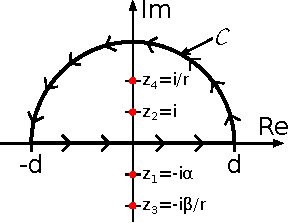
\includegraphics[width=7cm]{img/01_complex_contour.pdf}
 \caption{Closed integration contour $\mathcal{C}$ (thick black line) for application of the residue theorem
          and location of the poles $z_1, ..., z_4$ for $\alpha>0, \beta>0, r>0$ (red dots).}
\end{figure}
In order to recover the integral along the whole real axis,
the parameter $d$ of the integration contour $\mathcal{C}$ is taken to the limit $d \rightarrow +\infty$.
The order of the integrands $(1)$ to $(4)$ is $-2$ and thus the contribution from the great semicircle
to the contour integral vanishes, leaving only the contribution from the real axis,
which is equivalent (in the limit $d \rightarrow +\infty$) to the original $y$-integral.
The residue theorem on the other hand allows to express the contour integral
with the sum of the residuals (, i.e., poles) \underline{within} the contour $\mathcal{C}$.
Depending on the signs of $\alpha$, $\beta$ and $r$,
the poles of a given integrand $(1)$ to $(4)$ have $\imagpart(z_k)>0$ or $\imagpart(z_k)<0$ ($k=1,...,4$).
The contour $\mathcal{C}$ (parameterized by $d$) has to be taken large enough to include all poles $z_k$ with $\imagpart(z_k)>0$.
The calculation of the $y$ integrals over $(1)$ to $(4)$ then reduces to computation of the residuals of $z_1, ..., z_4$,
assuming that they are located within $\mathcal{C}$, and then summing them up with cases
for the various combinations of signs of $\alpha$, $\beta$ and $r$.
We start with $(1)$:
\begin{equation}
  \int\limits_{-\infty}^{+\infty}
    (1) \,\mathrm{d}y
= \oint_\mathcal{C}
    f_1(z) \,\mathrm{d}z \label{eqn:int_f1}
\end{equation}
with
\begin{align}
  f_1(z) =& \frac{1}{z + i \alpha}          \cdot \frac{1}{r z + i \beta} \\
         =& \frac{1}{z + i \frac{\beta}{r}} \cdot \frac{1}{r(z + i \alpha)} \, .
\end{align}
The residues of $f_1$ are:
\begin{align}
 \mathrm{res}_{z_1} f_1 =& \frac{1}{r(-i \alpha) + i \beta}
                        =  \frac{1}{-i \alpha r + i \beta}
                        =  \frac{1}{i(\beta - \alpha r)}
                        \textrm{ for } \alpha < 0 \Rightarrow \imagpart(-i\alpha) > 0 \\
 \mathrm{res}_{z_3} f_1 =& \frac{1}{r(-i \frac{\beta}{r} + i \alpha)}
                        =  \frac{1}{-i \beta + i \alpha r}
                        =  \frac{-1}{i(\beta - \alpha r)}
                        \textrm{ for } r>0, \beta< 0 \textrm{ or } r<0, \beta>0 \, .
\end{align}
The integral in \eqn{int_f1} can be evaluated:
\begin{equation}
   \oint_\mathcal{C} f_1(z) \,\mathrm{d}z
 = 2 \pi i \left[ \left\{ \begin{aligned}
                   \frac{1}{i(\beta-\alpha r)} :&\, \alpha<0 \\
                   0                           :&\, \alpha>0
                  \end{aligned} \right\}
                 +\left\{ \begin{aligned}
                   \frac{-1}{i(\beta-\alpha r)} :&\, \left\{\begin{aligned}
                                                       r>0,&\, \beta<0 \textrm{ or} \\
                                                       r<0,&\, \beta>0
                                                      \end{aligned} \right. \\
                   0                           :&\, \textrm{else}
                  \end{aligned} \right\}
 \right] \, .
\end{equation}
For the $y$-integral over $(1)$ four cases are therefore relevant regarding the signs of $\alpha$ and $\beta$:
\begin{align}
 \alpha>0, \beta>0 :&\, \int\limits_{-\infty}^{+\infty} (1) \,\mathrm{d}y = \begin{cases}
                                                                             \frac{-2\pi}{\beta-\alpha r} &:\, r<0 \\
                                                                             0                            &:\, r>0
                                                                            \end{cases} \\
 \alpha>0, \beta<0 :&\, \int\limits_{-\infty}^{+\infty} (1) \,\mathrm{d}y = \begin{cases}
                                                                             0                            &:\, r<0 \\
                                                                             \frac{-2\pi}{\beta-\alpha r} &:\, r>0
                                                                            \end{cases} \\
 \alpha<0, \beta>0 :&\, \int\limits_{-\infty}^{+\infty} (1) \,\mathrm{d}y = \begin{cases}
                                                                             0                            &:\, r<0 \\
                                                                             \frac{ 2\pi}{\beta-\alpha r} &:\, r>0
                                                                            \end{cases} \\
 \alpha<0, \beta<0 :&\, \int\limits_{-\infty}^{+\infty} (1) \,\mathrm{d}y = \begin{cases}
                                                                             \frac{ 2\pi}{\beta-\alpha r} &:\, r<0 \\
                                                                             0                            &:\, r>0
                                                                            \end{cases} \, .
\end{align}
Next, consider $(2)$:
\begin{equation}
  \int\limits_{-\infty}^{+\infty}
    (2) \,\mathrm{d}y
= \oint_\mathcal{C}
    f_2(z) \,\mathrm{d}z \label{eqn:int_f2}
\end{equation}
with
\begin{align}
  f_2(z) =& \frac{1}{z + i \alpha}    \cdot \frac{1}{r z - i} \\
         =& \frac{1}{z - \frac{i}{r}} \cdot \frac{1}{r(z + i \alpha)} \, .
\end{align}
The residues of $f_2$ are:
\begin{align}
 \mathrm{res}_{z_1} f_2 =& \frac{1}{r(-i \alpha)  - i}
                        =  \frac{1}{  -i \alpha r - i}
                        =  \frac{-1}{i(1 + \alpha r)}
                        \textrm{ for } \alpha < 0 \\
 \mathrm{res}_{z_4} f_2 =& \frac{1}{r(\frac{i}{r} + i \alpha)}
                        =  \frac{1}{i + i \alpha r}
                        =  \frac{1}{i(1 + \alpha r)}
                        \textrm{ for } r > 0\, .
\end{align}
The integral in \eqn{int_f2} can be evaluated:
\begin{equation}
   \oint_\mathcal{C} f_2(z) \,\mathrm{d}z
 = 2 \pi i \left[ \left\{ \begin{aligned}
                   \frac{-1}{i(1 + \alpha r)} :&\, \alpha<0 \\
                   0                          :&\, \alpha>0
                  \end{aligned} \right\}
                 +\left\{ \begin{aligned}
                   0                         :&\, r < 0 \\
                   \frac{1}{i(1 + \alpha r)} :&\, r > 0
                  \end{aligned} \right\}
 \right] \, .
\end{equation}
For the $y$-integral over $(2)$ two cases are therefore relevant regarding the sign of $\alpha$:
\begin{align}
 \alpha > 0 :&\, \int\limits_{-\infty}^{+\infty} (2) \,\mathrm{d}y = \begin{cases}
                                                                      0                        &:\, r<0 \\
                                                                      \frac{ 2\pi}{1+\alpha r} &:\, r>0
                                                                     \end{cases} \\
 \alpha < 0 :&\, \int\limits_{-\infty}^{+\infty} (2) \,\mathrm{d}y = \begin{cases}
                                                                      \frac{-2\pi}{1+\alpha r} &:\, r<0 \\
                                                                      0                        &:\, r>0
                                                                     \end{cases} \, .
\end{align}
We continue with $(3)$:
\begin{equation}
  \int\limits_{-\infty}^{+\infty}
    (3) \,\mathrm{d}y
= \oint_\mathcal{C}
    f_3(z) \,\mathrm{d}z \label{eqn:int_f3}
\end{equation}
with
\begin{align}
  f_3(z) =& \frac{1}{z - i}    \cdot \frac{1}{r z + i \beta} \\
         =& \frac{1}{z + i \frac{\beta}{r}} \cdot \frac{1}{r(z - i)} \, .
\end{align}
The residues of $f_3$ are:
\begin{align}
 \mathrm{res}_{z_2} f_3 =& \frac{1}{r i + i \beta}
                        =  \frac{1}{i (r + \beta)} \\
 \mathrm{res}_{z_3} f_3 =& \frac{1}{r(-i\frac{\beta}{r} - i)}
                        =  \frac{1}{-i \beta - i r}
                        =  \frac{-1}{i(\beta + r)}
                        \textrm{ for } r>0, \beta< 0 \textrm{ or } r<0, \beta>0 \, .
\end{align}
The integral in \eqn{int_f3} can be evaluated:
\begin{equation}
   \oint_\mathcal{C} f_3(z) \,\mathrm{d}z
 = 2 \pi i \left[ \frac{1}{i(\beta + r)} \\
                 +\left\{ \begin{aligned}
                   \frac{-1}{i(\beta + r)} :&\, \left\{\begin{aligned}
                                                       r>0,&\, \beta<0 \textrm{ or} \\
                                                       r<0,&\, \beta>0
                                                      \end{aligned} \right. \\
                   0                           :&\, \textrm{else}
                  \end{aligned} \right\}
 \right] \, .
\end{equation}
For the $y$-integral over $(3)$ two cases are therefore relevant regarding the sign of $\beta$:
\begin{align}
 \beta > 0 :&\, \int\limits_{-\infty}^{+\infty} (3) \,\mathrm{d}y = \begin{cases}
                                                                      0                      &:\, r<0 \\
                                                                      \frac{2\pi}{\beta + r} &:\, r>0
                                                                    \end{cases} \\
 \beta < 0 :&\, \int\limits_{-\infty}^{+\infty} (3) \,\mathrm{d}y = \begin{cases}
                                                                      \frac{2\pi}{\beta + r} &:\, r<0 \\
                                                                      0                      &:\, r>0
                                                                    \end{cases} \, .
\end{align}
Finally we consider the $y$-integral over $(4)$:
\begin{equation}
  \int\limits_{-\infty}^{+\infty}
    (4) \,\mathrm{d}y
= \oint_\mathcal{C}
    f_4(z) \,\mathrm{d}z \label{eqn:int_f4}
\end{equation}
with
\begin{align}
  f_4(z) =& \frac{1}{z - i}           \cdot \frac{1}{r z - i} \\
         =& \frac{1}{z - \frac{i}{r}} \cdot \frac{1}{r(z - i)} \, .
\end{align}
The residues of $f_4$ are:
\begin{align}
 \mathrm{res}_{z_2} f_4 =& \frac{1}{r i -i}
                        =  \frac{1}{i (r - 1)} \\
 \mathrm{res}_{z_4} f_4 =& \frac{1}{r(\frac{i}{r} - i)}
                        =  \frac{1}{i(1 - r)}
                        =  \frac{-1}{i(r - 1)}
                        \textrm{ for } r>0 \, .
\end{align}
The integral in \eqn{int_f4} can be evaluated:
\begin{equation}
   \oint_\mathcal{C} f_4(z) \,\mathrm{d}z
 = 2 \pi i \left[ \frac{1}{i(r - 1)} \\
                 +\left\{ \begin{aligned}
                   0                   :&\, r < 0 \\
                   \frac{-1}{i(r - 1)} :&\, r > 0
                  \end{aligned} \right\}
 \right] \, .
\end{equation}
The $y$-integral over $(4)$ is thus:
\begin{equation}
   \int\limits_{-\infty}^{+\infty} (4) \,\mathrm{d}y
 = \begin{cases}
    \frac{2 \pi}{r-1} &:\, r<0 \\
    0                 &:\, r>0
   \end{cases} \, .
\end{equation}
The $y$-integrals are now complete. The results are inserted back into the remaining
integral over $r$ and the cases for different signs of $r$ are evaluated to limit the ranges of the integrals over $r$.
We need to consider $\alpha>0$, $\beta>0$ for compatibility with earlier assumptions
regarding $s$ and $t$ in \eqn{geom_series_s} and \eqn{geom_series_t}:
\begin{align}
 I&(s,t) = \frac{-1}{4 \pi}
           \int\limits_{-\infty}^{+\infty}
            \frac{\mathrm{d}r}
                 {\sqrt{a + 2 b r + c r^2}}  \nonumber \\
   ~     &  \left[
             \left\{\begin{aligned}
              \frac{-2\pi}{\beta-\alpha r} &:\, r<0 \\
              0                            &:\, r>0
             \end{aligned}\right\}
           - \left\{\begin{aligned}
              0                        &:\, r<0 \\
              \frac{ 2\pi}{1+\alpha r} &:\, r>0
             \end{aligned}\right\}
           - \left\{\begin{aligned}
               0                      &:\, r<0 \\
               \frac{2\pi}{\beta + r} &:\, r>0
             \end{aligned}\right\}
           + \left\{\begin{aligned}
              \frac{2 \pi}{r-1} &:\, r<0 \\
              0                 &:\, r>0
             \end{aligned}\right\}
           \right] \, . \nonumber \\
 =& \frac{-1}{4 \pi}
    \int\limits_{-\infty}^{0}
      \left[ \frac{-2 \pi}{\beta - \alpha r} + \frac{2 \pi}{r - 1} \right]
      \frac{\mathrm{d}r}
           {\sqrt{a + 2 b r + c r^2}}
  + \frac{1}{4 \pi}\int\limits_{0}^{+\infty}
      \left[ \frac{2 \pi}{1 + \alpha r} + \frac{2 \pi}{\beta + r} \right]
      \frac{\mathrm{d}r}
           {\sqrt{a + 2 b r + c r^2}} \nonumber \\
 =& \frac{1}{2}
    \int\limits_{0}^{-\infty}
      \left[ \frac{-1}{\beta - \alpha r} + \frac{1}{r - 1} \right]
      \frac{\mathrm{d}r}
           {\sqrt{a + 2 b r + c r^2}}
  + \frac{1}{2}\int\limits_{0}^{+\infty}
      \left[ \frac{1}{1 + \alpha r} + \frac{1}{\beta + r} \right]
      \frac{\mathrm{d}r}
           {\sqrt{a + 2 b r + c r^2}} \nonumber \\
 =& \frac{1}{2}
    \int\limits_{0}^{+\infty}
      \left[ \frac{-1}{\beta - \alpha (-r)} + \frac{1}{(-r) - 1} \right]
      \frac{-\mathrm{d}r}
           {\sqrt{a - 2 b r + c r^2}}
  + \frac{1}{2}\int\limits_{0}^{+\infty}
      \left[ \frac{1}{1 + \alpha r} + \frac{1}{\beta + r} \right]
      \frac{\mathrm{d}r}
           {\sqrt{a + 2 b r + c r^2}} \nonumber \\
 =& \frac{1}{2}
    \int\limits_{0}^{+\infty}
      \left[ \frac{1}{\beta + \alpha r} + \frac{1}{1 + r} \right]
      \frac{\mathrm{d}r}
           {\sqrt{a - 2 b r + c r^2}}
  + \frac{1}{2}\int\limits_{0}^{+\infty}
      \left[ \frac{1}{1 + \alpha r} + \frac{1}{\beta + r} \right]
      \frac{\mathrm{d}r}
           {\sqrt{a + 2 b r + c r^2}} \, . \label{eqn:int_I_split}
\end{align}
A change of variables is performed from $r$ to $x$ with
\begin{equation}
  x = \frac{r - 1}{r + 1} \, .
\end{equation}
Note that for this change of variables the Jacobian is:
\begin{equation}
 \frac{\mathrm{d}x}{\mathrm{d}r} = \frac{2}{(r+1)^2} ~ \Rightarrow ~ \mathrm{d}x = \frac{2 \,\mathrm{d}r}{(r+1)^2} \, .
\end{equation}
In \eqn{int_I_split} four relatively similar terms occur:
\begin{align}
 \frac{1}{\beta + \alpha r} ~& \qquad \qquad \qquad \quad (\textrm{the original}), \nonumber \\
 \frac{1}{1 + r}            =& \left. \frac{1}{\beta + \alpha r} \right|_{\alpha = 1,
                                                                          \beta  = 1} \, , \nonumber \\
 \frac{1}{1 + \alpha r}     =& \left. \frac{1}{\beta + \alpha r} \right|_{\beta  = 1} \qquad \textrm{and} \nonumber \\
 \frac{1}{\beta + r}        =& \left. \frac{1}{\beta + \alpha r} \right|_{\alpha = 1} \qquad . \nonumber
\end{align}
Therefore it is sufficient to consider the original term only and the others will follow from it.
Furthermore, $\alpha$ and $\beta$ are replaced again with their respective expressions in $s$ and $t$:
\begin{equation}
  s = \frac{1 - \alpha}{1 + \alpha} \quad \mathrm{and} \quad t = \frac{1 - \beta}{1 + \beta} \, ,
\end{equation}
leading to
\begin{align}
  \left( \beta + \alpha r \right)^{-1}
  =& \left( \frac{1-t}{1+t} + \frac{1-s}{1+s} \,r \right)^{-1}
  =  \left( \frac{(1-t)(1+s) + (1+t)(1-s) r}{(1+t)(1+s)} \right)^{-1} \nonumber \\
  =& \frac{(1+t)(1+s)}{1 +s-t -st +r -sr+tr -str}
  =  \frac{(1+t)(1+s)}{(r+1)-st(r+1)-(s-t)(r-1)} \label{eqn:beta_alpha_r} \\
  =& \frac{1}{r+1} \cdot \frac{(1+t)(1+s)}{1-st-(s-t)\underbrace{\frac{r-1}{r+1}}_{=\,x}}
  =  \frac{1}{r+1} \cdot \frac{(1+t)(1+s)}{1-st-(s-t)x} \nonumber
\end{align}
where $\alpha=1$ implies $s=0$ and $\beta=1$ implies $t=0$.
Next consider the argument of the inverse square roots in \eqn{int_I_split}.
New variables are introduced:
\begin{align}
 a^{+} =&\, a + 2b + c \nonumber \\
 a^{-} =&\, a - 2b + c \\
 d     =&\, c - a \nonumber
\end{align}
which can be solved for the old variables $a$, $b$, $c$ as follows:
\begin{align}
 b =&\, \frac{1}{4} \left( a^{+} - a^{-} \right) \nonumber \\
 a =&\, \frac{1}{4} \left( a^{+} + a^{-} - 2d \right) \\
 c =&\, \frac{1}{4} \left( a^{+} + a^{-} + 2d \right) \nonumber
\end{align}
Inserting these expressions into the inverse square root argument results in:
\begin{align}
 a \pm 2 b r + c r^2
 =&\, \frac{1}{4} \left[ \left( a^{+} + a^{-} - 2d \right) \pm 2 \left( a^{+} - a^{-} \right) r + \left( a^{+} + a^{-} + 2d \right) r^2 \right] \nonumber \\
 =&\, \frac{1}{4} \left[ a^{+} + a^{-} - 2d \pm 2ra^{+} \mp 2ra^{-} + r^2a^{+} + r^2a^{-} + 2r^2d \right] \nonumber \\
 =&\, \frac{1}{4} \left[ \left( 1 \pm 2r + r^2 \right) a^{+}  + 2 \left( r^2 - 1 \right) d + \left( 1 \mp 2r + r^2 \right) a^{-} \right] \nonumber \\
 =&\, \frac{1}{4} \left[ \left( r \pm 1 \right)^2 a^{+}  + 2 (r-1)(r+1) d + \left( r \mp 1 \right)^2 a^{-} \right] \label{eqn:a_pm_etc} \\
 =&\, \frac{1}{4} (r+1)^2 \Biggl[ a^{\pm}  + 2 \underbrace{\frac{r-1}{r+1}}_{=\,x} d + \Biggl( \underbrace{\frac{r-1}{r+1}}_{=\,x} \Biggr)^2 a^{\mp} \Biggr] \nonumber \\
 =&\, \frac{1}{4} (r+1)^2 \left( a^{\pm}  + 2 d x + a^{\mp} x^2 \right) \, . \nonumber
\end{align}

Now \eqn{beta_alpha_r} and \eqn{a_pm_etc} can be substitited back into \eqn{int_I_split}:
\begin{align}
 I(s,t)
 =& \phantom{+}\,
     \frac{1}{2} \int\limits_{0}^{+\infty}
     \frac{1}{r+1}
     \left(
         \frac{(1+t)(1+s)}{1-st-(s-t)x}
       + 1
     \right)
     \frac{\mathrm{d}r}{\frac{1}{2} (r+1) \sqrt{ a^{-}  + 2 d x + a^{+} x^2 }} \nonumber \\
 ~& +
     \frac{1}{2} \int\limits_{0}^{+\infty}
     \frac{1}{r+1}
     \left(
         \frac{1+s}{1-sx}
       + \frac{1+t}{1+tx}
     \right)
     \frac{\mathrm{d}r}{\frac{1}{2} (r+1) \sqrt{ a^{+}  + 2 d x + a^{-} x^2 }} \nonumber \\
 =& \phantom{+}\,
     \frac{1}{2} \int\limits_{0}^{+\infty}
     \underbrace{\frac{2 \,\mathrm{d}r}{(r+1)^2}}_{=\mathrm{d}x}
     \left(
         \frac{(1+t)(1+s)}{1-st-(s-t)x}
       + 1
     \right)
     \frac{1}{\sqrt{ a^{-}  + 2 d x + a^{+} x^2 }} \nonumber \\
 ~& +
     \frac{1}{2} \int\limits_{0}^{+\infty}
     \underbrace{\frac{2 \,\mathrm{d}r}{(r+1)^2}}_{=\mathrm{d}x}
     \left(
         \frac{1+s}{1-sx}
       + \frac{1+t}{1+tx}
     \right)
     \frac{1}{\sqrt{ a^{+}  + 2 d x + a^{-} x^2 }} \, .
\end{align}
With this it follows for $I(s,t)$:
\begin{align}
 I(s,t)
 =& \phantom{+}\,
     \frac{1}{2} \int\limits_{-1}^{1}
     \left(
         \frac{(1+t)(1+s)}{1-st-(s-t)x}
       + 1
     \right)
     \frac{\mathrm{d}x}{\sqrt{ a^{-}  + 2 d x + a^{+} x^2 }} \nonumber \\
 ~& +
     \frac{1}{2} \int\limits_{-1}^{1}
     \left(
         \frac{1+s}{1-sx}
       + \frac{1+t}{1+tx}
     \right)
     \frac{\mathrm{d}x}{\sqrt{ a^{+}  + 2 d x + a^{-} x^2 }} \, .
\end{align}
The following function $h^{\pm}(s,t)$ is introduced:
\begin{equation}
   h^{\pm}(s,t)
 = \frac{(1+s)(1+t)}{2}
   \int\limits_{-1}^{1}
     \frac{\mathrm{d}x}{\left( 1-st-(s-t)x \right)\sqrt{ a^{\mp}  + 2 d x + a^{\pm} x^2 }}
\end{equation}
and $I(s,t)$ can be expressed using $h^{\pm}(s,t)$ as follows:
\begin{equation}
 I(s,t) = h^{+}(s,t) + h^{+}(0,0) + h^{-}(s,0) + h^{-}(0,t) \, . \label{eqn:I_from_h}
\end{equation}
Now consider $h^{\pm}(s,t)$ in more detail:
\begin{align}
 h^{\pm}(s,t)
 =&\, \frac{(1+s)(1+t)}{2}
    \int\limits_{-1}^{1}
     \frac{\mathrm{d}x}{\underbrace{\left( 1-st-(s-t)x \right)}_{\begin{aligned}
            =& (1-st)\left(1- \frac{s-t}{1-st} x \right)
            \end{aligned}}\sqrt{ a^{\mp}  + 2 d x + a^{\pm} x^2 }} \nonumber \\
 =&\, \frac{1}{2}
    \frac{(1+s)(1+t)}{1-st}
    \int\limits_{-1}^{1}
    \underbrace{\frac{1}{1- \frac{s-t}{1-st} x}}_{\begin{aligned}
                      = \sum\limits_{l=0}^{\infty} \left( \frac{s-t}{1-st} \right)^l x^l
                                                          \end{aligned}}
     \frac{\mathrm{d}x}{\sqrt{ a^{\mp}  + 2 d x + a^{\pm} x^2 }} \nonumber \\
 =&\, \frac{1}{2}
    \frac{(1+s)(1+t)}{1-st}
    \int\limits_{-1}^{1}
      \sum\limits_{l=0}^{\infty} \left( \frac{s-t}{1-st} \right)^l
      \frac{x^l}{\sqrt{ a^{\mp}  + 2 d x + a^{\pm} x^2 }}
      \,\mathrm{d}x \nonumber \\
 =&\, \frac{1}{2}
    \frac{(1+s)(1+t)}{1-st}
    \sum\limits_{l=0}^{\infty} \left( \frac{s-t}{1-st} \right)^l
    \int\limits_{-1}^{1}
      \frac{x^l}{\sqrt{ a^{\mp}  + 2 d x + a^{\pm} x^2 }}
      \,\mathrm{d}x \nonumber \\
 =&\, \frac{1}{2}
    \frac{(1+s)(1+t)}{1-st}
    \sum\limits_{l=0}^{\infty} \left( \frac{s-t}{1-st} \right)^l
    T^{\pm}_l \label{eqn:h_pm_st}
\end{align}
with
\begin{equation}
 T^{\pm}_l
 = \int\limits_{-1}^{1}
      \frac{x^l}{\sqrt{ a^{\mp}  + 2 d x + a^{\pm} x^2 }}
      \,\mathrm{d}x \, . \label{eqn:T_pm_l}
\end{equation}
The last three terms of \eqn{I_from_h} can be simplified already:
\begin{align}
  h^{+}(0,0) =& \frac{1}{2} T^{+}_0 \label{eqn:h_p_00} \\
  h^{-}(s,0) =& \frac{1}{2} (1+s) \sum\limits_{l=0}^{+\infty} s^l T^{-}_l
             =  \frac{1}{2} \left[ \sum\limits_{l=0}^{+\infty} T^{-}_l s^l + \sum\limits_{l=0}^{+\infty} T^{-}_l s^{l+1} \right] \nonumber \\
      ~      =& \frac{1}{2} T^{-}_0 + \frac{1}{2} \sum\limits_{l=1}^{+\infty} \left( T^{-}_l + T^{-}_{l-1} \right) s^l \label{eqn:h_m_s0} \\
  h^{-}(0,t) =& \frac{1}{2} (1+t) \sum\limits_{l=0}^{+\infty} (-t)^l T^{-}_l
             =  \frac{1}{2} \left[ \sum\limits_{l=0}^{+\infty} (-1)^l T^{-}_l t^l + \sum\limits_{l=0}^{+\infty} (-1)^l T^{-}_l t^{l+1} \right] \nonumber \\
      ~      =& \frac{1}{2} T^{-}_0 + \frac{1}{2} \sum\limits_{l=1}^{+\infty} (-1)^l \left( T^{-}_l - T^{-}_{l-1} \right) t^l \label{eqn:h_m_0t} \, .
\end{align}
Equation~(\ref{eqn:h_pm_st}) can be further expanded for $h^{+}(s,t)$:
\begin{align}
 h^{+}(s,t)
 =& \frac{(1+s)(1+t)}{2}
    \sum\limits_{l=0}^{+\infty} (s-t)^l \frac{1}{(1-st)^{l+1}} T^{+}_l \nonumber \\
 =& \frac{(1+s)(1+t)}{2}
    \sum\limits_{l=0}^{+\infty}
      \left( \sum\limits_{j=0}^{l} (-1)^{j} {\genfrac(){0pt}{0}{l}{j}} s^{l-j} t^{j} \right)
      \left( \sum\limits_{k=0}^{+\infty} {\genfrac(){0pt}{0}{k+l}{k}} s^k t^k \right)
      \,T^{+}_l \nonumber \\
 =& \frac{(1+s)(1+t)}{2}
    \sum\limits_{k=0}^{+\infty}
    \sum\limits_{l=0}^{+\infty}
    \sum\limits_{j=0}^{l}
      (-1)^{j}
      \frac{\bcancel{l!}\,(k+l)!}{j!\,(l-j)!\,k!\,\bcancel{l!}}
      \,T^{+}_l
      s^{k+l-j} t^{k+j} \nonumber \\
 =& \frac{1}{2} (1+s+t+st)
    \sum\limits_{k=0}^{+\infty}
    \sum\limits_{l=0}^{+\infty}
    \sum\limits_{j=0}^{l}
      (-1)^{j}
      \frac{(k+l)!}{j!\,(l-j)!\,k!}
      \,T^{+}_l
      s^{k+l-j} t^{k+j} \label{eqn:h_p_st} \, .
\end{align}
The representation of $I(s,t)$ from \eqn{I_from_h} is equated with the representation from \eqn{I_gf}.
The goal now is to identify which terms from \eqn{h_p_00}, \eqn{h_m_s0}, \eqn{h_m_0t} and \eqn{h_p_st}
contribute to $I_{m,n}$ for any given powers $m$ and $n$ of $s$ and $t$, respectively.
The contributions from $h^{+}(0,0)$, $h^{-}(s,0)$ and $h^{-}(0,t)$ are easily related to $(m=0, n=0)$, $(m=0, n\geq1)$ and $(m\geq1, n=0)$.
The contributions from $h^{+}(s,t)$ are a little bit more involved
and thus, only the sums
\begin{equation}
  \sum\limits_{k=0}^{+\infty}
  \sum\limits_{l=0}^{+\infty}
  \sum\limits_{j=0}^{l}
    (-1)^{j}
    \frac{(k+l)!}{j!\,(l-j)!\,k!}
    \,T^{+}_l
    s^{k+l-j} t^{k+j} \label{eqn:sums_h_p_st}
\end{equation}
are considered for now.
For the following, assume $m\geq1$ and $n\geq1$ are given. The task is now to find all terms in \eqn{sums_h_p_st} with matching $s^m$ and $t^n$.
There exist two cases, namely $m \geq n$ and $n \geq m$.

Assume $m \geq n$ for the first part.
Then there are $(n+1)$ contributions to $s^m t^n$ with $m=k+l-j$ and $n=k+j$,
since $k \geq 0$ and $j \geq 0$, leading to the list of possible combinations of values of $j$ and $k$ shown in Tab.~(\ref{tab:from_j_k_to_n}).
\begin{table}[htbp]
  \centering
  \begin{tabular}{c|c}
    $j$ & $k$ \\
    \hline
    0 & $n$ \\
    1 & $n-1$ \\
    ... & ... \\
    $n-1$ & 1 \\
    $n$ & 0
  \end{tabular}
  \caption{$(n+1)$ possible combinations of $j \geq 0$ and $k \geq 0$ which sum up to a given $n=k+j$.}
  \label{tab:from_j_k_to_n}
\end{table}
For every row in Tab.~(\ref{tab:from_j_k_to_n}) (indexed by $j=0, 1, ..., n$), the appropriate value of $k$ is given by $k=n-j$.
Then, $l$ has to be chosen sufficiently large, so that $m=k+l-j$ is fulfilled.
For the given $m$ and a given $j$ and appropriately chosen $k~(=n-j$, see above), the matching value
of $l$ is $l=m-k+j$ and inserting the chosen value for $k$ into this leads to $l=m-n+2j$.

Now assume $n \geq m$ for the second part.
There are $(m+1)$ contributions to $s^m t^n$ with $m=k+l-j$ and $n=k+j$,
labeled $k=0, 1, ..., m$, as shown in Tab.~(\ref{tab:from_k_lmj_to_m}).
\begin{table}[htbp]
  \centering
  \begin{tabular}{c|c}
    $k$ & $l-j$ \\
    \hline
    0 & $m$ \\
    1 & $m-1$ \\
    ... & ... \\
    $m-1$ & 1 \\
    $m$ & 0
  \end{tabular}
  \caption{$(m+1)$ possible combinations of $k \geq 0$ and $l \geq 0$, $0 \leq j \leq l$ which sum up to a given $m=k+l-j$.}
  \label{tab:from_k_lmj_to_m}
\end{table}
For the given $n$, $j$ has to be chosen for $n=k+j$ as $j=n-k$.
Note that due to $n \geq m$ and $k \leq m$, $j \geq 0$ is guaranteed for above values of $k$.
Since $l \geq 0$ and $0 \leq j \leq l$ hold, it follows that $(l-j) \geq 0$ for any occuring values of $l$ and $j$.
Then, $l$ has to be found for the representation of $m$ from $m=k+l-j$.
Insert the chosen value for $j$ into $m$ as $m=k+l-(n-k) = k+l-n+k = l-n+2k$
and solve for $l$ as $l=m+n-2k$.
The value of $k$ takes on a maximum of $m$ and at this limit, the minimal value of $l$ occurs:
$l_\textrm{min} = m+n-2m = n-m$ and since $n \geq m$ was assumed, $l_\textrm{min} \geq 0$ is guaranteed.

For the two cases $m \geq n$ and $n \geq m$, the values of $k, l$ and $j,l$, respectively, are inserted into the summands in \eqn{sums_h_p_st}
and the contributions are summed up.
For the case of $m \geq n$, this leads to:
\begin{align}
     c^{+}_{m,n} s^m t^n
  :=& \frac{1}{2}
      \sum\limits_{j=0}^{n}
    (-1)^{j}
    \frac{(\bcancel{n}\bcancel{-j}+m\bcancel{-n}+\bcancel{2}j)!}{j!\,(m-n+\bcancel{2}j\bcancel{-j})!\,(n-j)!}
    \,T^{+}_{m-n+2j}
    s^{\bcancel{n}\bcancel{-j}+m\bcancel{-n}\bcancel{+2j}\bcancel{-j}} t^{n\bcancel{-j}\bcancel{+j}} \nonumber \\
 =& \frac{1}{2}
    \sum\limits_{j=0}^{n}
    (-1)^{j}
    \frac{(m+j)!}{j!\,(m-n+j)!\,(n-j)!}
    \,T^{+}_{m-n+2j}
    s^m t^n \, . \label{eqn:c_mn_mgeqn}
\end{align}
For the case of $n \geq m$, this leads to:
\begin{align}
     c^{+}_{m,n} s^m t^n
  :=& \frac{1}{2}
      \sum\limits_{k=0}^{m}
    (-1)^{n-k}
    \frac{(\bcancel{k}+m+n-\bcancel{2}k)!}{(n-k)!\,(m\bcancel{+n}-\bcancel{2}k\bcancel{-n}\bcancel{+k})!\,k!}
    \,T^{+}_{m+n-2k}
    s^{\bcancel{k}+m\bcancel{+n}\bcancel{-2k}\bcancel{-n}\bcancel{+k}} t^{\bcancel{k}+n\bcancel{-k}} \nonumber \\
  =& \frac{1}{2}
     \sum\limits_{k=0}^{m}
    (-1)^{n-k}
    \frac{(m+n-k)!}{(n-k)!\,(m-k)!\,k!}
    \,T^{+}_{m+n-2k}
    s^m t^n \nonumber \\
  \xrightarrow[k \rightarrow (m-k)]{(m-k) \rightarrow k} ~
  =& \frac{1}{2}
     \sum\limits_{k=0}^{m}
    (-1)^{k+n-m}
    \frac{(n+k)!}{(n-m+k)!\,k!\,(m-k)!}
    \,T^{+}_{n-m+2k}
    s^m t^n \, . \label{eqn:c_mn_ngeqm}
\end{align}
Comparing the two expressions from \eqn{c_mn_mgeqn} and from \eqn{c_mn_ngeqm} with either $m \geq n$  or $n \geq m$, respectively,
in mind, a generalization of the integer quantities in the $c^{+}_{m,n}$ can be found and is tabulated in Tab.~(\ref{tab:generalization_c_mn}).
\begin{table}[htbp]
  \centering
  \begin{tabular}{c | c | c | c}
    quantity                     & $m \geq n$ & $n \geq m$ & generally                 \\
    \hline
                     end of loop & $n$        & $m$        & $\mathrm{min}\,(m,n)$     \\
                 power of $(-1)$ & $j$        & $j+n-m$    & $\mathrm{max}\,(0, n-m)$  \\
          factorial in numerator & $j+m$      & $j+n$      & $j+\mathrm{max}\,(m,n)$   \\
    1st factorial in denominator & $n-j$      & $m-j$      & $\mathrm{min}\,(m,n) - j$ \\
    2nd factorial in denominator & $m-n+j$    & $n-m+j$    & $|m-n|+j$                 \\
                index of $T^{+}$ & $m-n+2j$   & $n-m+2j$   & $|m-n|+2j$
  \end{tabular}
  \caption{Generalization of the integer quantities in $c^{+}_{m,n}$.}
  \label{tab:generalization_c_mn}
\end{table}

The min/max functions can be expressed analytically:
\begin{align}
  \mathrm{min}\,(m,n)
  =& \frac{1}{2} (m+n-|m-n|) = \begin{cases}
                                 \frac{1}{2} (\bcancel{m}+n\bcancel{-m}+n) = n & ~:~ m \geq n \\
                                 \frac{1}{2} (m\bcancel{+n}\bcancel{-n}+m) = m & ~:~ n \geq m
                               \end{cases} \\
  \mathrm{max}\,(m,n)
  =& \frac{1}{2} (m+n+|m-n|) = \begin{cases}
                                 \frac{1}{2} (m\bcancel{+n}+m\bcancel{-n}) = m & ~:~ m \geq n \\
                                 \frac{1}{2} (\bcancel{m}+n+n\bcancel{-m}) = n & ~:~ n \geq m
                               \end{cases} \\
  \mathrm{max}\,(0,n-m)
  =& \frac{1}{2} (|m-n|-m+n) = \begin{cases}
                                 \frac{1}{2} (\bcancel{m}\bcancel{-n}\bcancel{-m}\bcancel{+n}) = 0 & ~:~ m \geq n \\
                                 \frac{1}{2} (n-m-m+n) = n-m & ~:~ n \geq m
                               \end{cases}
\end{align}
These expressions now can be inserted into $c^{+}_{m,n}$ and are valid for both $m \geq n$ and $n \geq m$:
\begin{equation}
    c^{+}_{m,n}
  = \frac{1}{2}
    \sum\limits_{j=0}^{\frac{m+n-|m-n|}{2}}
      (-1)^{j+\frac{|m-n|-m+n}{2}}
      \frac{\left(\frac{m+n+|m-n|}{2} +j \right)!}
           {\left(\frac{m+n-|m-n|}{2} -j \right)!\, (|m-n|+j)!\, j!}
      T^{+}_{|m-n|+2j} \, . \label{eqn:c_p_mn}
\end{equation}
The coefficients $c^{+}_{m,n}$ can now be used to express $h^{+}(s,t)$ from \eqn{h_p_st} again:
\begin{align}
 h^{+}&(s,t)
 = \, (1+s+t+st)
    \sum\limits_{m=0}^{+\infty}
    \sum\limits_{n=0}^{+\infty}
      c^{+}_{m,n}
      s^m t^n \nonumber \\
 =&   \sum\limits_{m=0}^{+\infty}
      \sum\limits_{n=0}^{+\infty}
        c^{+}_{m,n}
        s^m t^n
    + \sum\limits_{m=0}^{+\infty}
      \sum\limits_{n=0}^{+\infty}
        c^{+}_{m,n}
        s^{m+1} t^n
    + \sum\limits_{m=0}^{+\infty}
      \sum\limits_{n=0}^{+\infty}
        c^{+}_{m,n}
        s^m t^{n+1}
    + \sum\limits_{m=0}^{+\infty}
      \sum\limits_{n=0}^{+\infty}
        c^{+}_{m,n}
        s^{m+1} t^{n+1}            \nonumber \\
 =& \phantom{+} \,   c^{+}_{0,0}
                   + \sum\limits_{m=1}^{+\infty}
                       c^{+}_{m,0}
                       s^m
                   + \sum\limits_{n=1}^{+\infty}
                       c^{+}_{0,n}
                       t^n
                   + \sum\limits_{m=1}^{+\infty}
                     \sum\limits_{n=1}^{+\infty}
                       c^{+}_{m,n}
                       s^m t^n    \nonumber \\
 ~& + \sum\limits_{m=1}^{+\infty}
        c^{+}_{m-1,0}
        s^m
    + \sum\limits_{m=1}^{+\infty}
      \sum\limits_{n=1}^{+\infty}
        c^{+}_{m-1,n}
        s^m t^n                   \nonumber \\
 ~& + \sum\limits_{n=1}^{+\infty}
        c^{+}_{0,n-1}
        t^n
    + \sum\limits_{m=1}^{+\infty}
      \sum\limits_{n=1}^{+\infty}
        c^{+}_{m,n-1}
        s^m t^n                   \nonumber \\
 ~& + \sum\limits_{m=1}^{+\infty}
      \sum\limits_{n=1}^{+\infty}
        c^{+}_{m-1,n-1}
        s^m t^n                   \nonumber \\
 =& \phantom{+}\, \,c^{+}_{0,0}   \nonumber \\
 ~&          +  \sum\limits_{n=1}^{+\infty}
                  \left( c^{+}_{0,n} + c^{+}_{0,n-1} \right)
                  t^n             \nonumber \\
 ~&          +  \sum\limits_{m=1}^{+\infty}
                  \left( c^{+}_{m,0} + c^{+}_{m-1,0} \right)
                  s^m             \nonumber \\
 ~&          +  \sum\limits_{m=1}^{+\infty}
                \sum\limits_{n=1}^{+\infty}
                  \left( c^{+}_{m,n} + c^{+}_{m-1,n} + c^{+}_{m,n-1} + c^{+}_{m-1,n-1} \right)
                  s^m t^n \label{eqn:h_p_st_c_mn}
\end{align}
As it turns out, the expression for $c^{+}_{m,n}$ in \eqn{c_p_mn}
generalizes further to $c^{\pm}_{m,n}$ for $m \geq 0$ and $n \geq 0$:
\begin{equation}
    c^{\pm}_{m,n}
  := \frac{1}{2}
    \sum\limits_{j=0}^{\frac{m+n-|m-n|}{2}}
      (-1)^{j+\frac{|m-n|-m+n}{2}}
      \frac{\left(\frac{m+n+|m-n|}{2} +j \right)!}
           {\left(\frac{m+n-|m-n|}{2} -j \right)!\, (|m-n|+j)!\, j!}
      T^{\pm}_{|m-n|+2j} \, . \label{eqn:c_pm_mn}
\end{equation}
First, evaluate $c^{\pm}_{m,n}$ for $m=0$ and $n=0$:
\begin{equation}
  c^{\pm}_{0,0} = \frac{1}{2} T^{\pm}_0 \, .
\end{equation}
Next, consider the case of $m=0$ and $n \geq 1$:
\begin{equation}
  c^{\pm}_{0,n} = \frac{1}{2} (-1)^n \,T^{\pm}_n
\end{equation}
and similarly for $m \geq 1$ and $n=0$:
\begin{equation}
  c^{\pm}_{m,0} = \frac{1}{2} \,T^{\pm}_m \, .
\end{equation}
These terms can be found in \eqn{h_p_00}, \eqn{h_m_s0} and \eqn{h_m_0t}:
\begin{align}
  h^{+}(0,0) =& c^{+}_{0,0} \label{eqn:h_p_00_c_mn} \\
  h^{-}(s,0) =& c^{-}_{0,0} + \sum\limits_{m=1}^{+\infty} \left( c^{-}_{m,0} + c^{-}_{m-1,0} \right) s^m \label{eqn:h_m_s0_c_mn} \\
  h^{-}(0,t) =& c^{-}_{0,0} + \sum\limits_{n=1}^{+\infty} \left( c^{-}_{0,n} + c^{-}_{0,n-1} \right) t^n \label{eqn:h_m_0t_c_mn} \, .
\end{align}
Remember the two representations of $I(s,t)$ from \eqn{I_gf} and \eqn{I_from_h}:
\begin{equation*}
 I(s,t) = \sum\limits_{m=0}^{+\infty}
          \sum\limits_{n=0}^{+\infty}
            I_{m,n} s^m t^n
        = h^{+}(s,t) + h^{+}(0,0) + h^{-}(s,0) + h^{-}(0,t)
        \, .
\end{equation*}
Collecting terms with equal powers of $s$ and $t$
from \eqn{h_p_st_c_mn}, \eqn{h_p_00_c_mn}, \eqn{h_m_s0_c_mn} and \eqn{h_m_0t_c_mn}
finally leads to the following form of the $I_{m,n}$ coefficients:
\begin{equation}
 I_{m,n} = \left\{
           \begin{array}{lllll}
             c^{+}_{m,n} &+\, c^{+}_{m-1,n} &+\, c^{+}_{m,n-1} &+\, c^{+}_{m-1,n-1} &\textrm{for}~~ m \geq 1 , n \geq 1 \\
             c^{+}_{m,0} &+\, c^{+}_{m-1,0} &+\, c^{-}_{m,0}   &+\, c^{-}_{m-1,0}   &\textrm{for}~~ m \geq 1 , n = 0 \\
             c^{+}_{0,n} &+\, c^{+}_{0,n-1} &+\, c^{-}_{0,n}   &+\, c^{-}_{0,n-1}   &\textrm{for}~~ m = 0    , n \geq 1 \\
             c^{+}_{0,0} &+\, c^{+}_{0,0}   &+\, c^{-}_{0,0}   &+\, c^{-}_{0,0}     &\textrm{for}~~ m = 0    , n = 0 \, .
           \end{array} \right. \label{eqn:Imn}
\end{equation}

\FloatBarrier
\subsection{Closed Form Expressions for the Coefficients}
Next, find closed form expressions for the coefficients $T^{\pm}_l$ from \eqn{T_pm_l}.
The first case for $l=0$ is:
\begin{equation}
 T^{\pm}_0 = \int\limits_{-1}^{1} \frac{\mathrm{d}x}{\sqrt{ a^{\mp}  + 2 d x + a^{\pm} x^2 }}
\end{equation}
The corresponding antiderivative is tabulated in Ref.~\cite{gradshteyn_ryzhik} labeled 2.261.
The following shorthand notations are needed:
\begin{align}
      R =& {a'} + {b'} x + {c'} x^2 \label{eqn:def_R} \\
 \Delta =& 4 {a'} {c'} - {b'}^2 \label{eqn:def_delta}
\end{align}
with
\begin{align}
 {a'} =& a^{\mp} = a \mp 2 b + c \nonumber \\
 {b'} =& 2 d = 2 (c-a) \label{eqn:def_primes} \\
 {c'} =& a^{\pm} = a \pm 2 b + c \nonumber \, ,
\end{align}
where $a$, $b$ and $c$ are from \eqn{def_abc}:
\begin{equation}
 \begin{array}{llll}
 a &= {\mathbf{x}'}_{u'}^2 &= {\mathbf{x}'}_{u'} \cdot {\mathbf{x}'}_{u'} &= |{\mathbf{x}'}_{u'}|^2\\
 b &        ~              &= {\mathbf{x}'}_{u'} \cdot {\mathbf{x}'}_{v'} &= |{\mathbf{x}'}_{u'}| \cdot |{\mathbf{x}'}_{v'}| \cdot \cos(\theta) \\
 c &= {\mathbf{x}'}_{v'}^2 &= {\mathbf{x}'}_{v'} \cdot {\mathbf{x}'}_{v'} &= |{\mathbf{x}'}_{v'}|^2
 \end{array}
\end{equation}
where $\theta$ is the angle between ${\mathbf{x}'}_{u'}$ and ${\mathbf{x}'}_{v'}$.
The signs of $c'$ and $\Delta$ need to be considered for selecting which antiderivative can be used.
It follows for $c'$:
\begin{equation}
 {c'} = |{\mathbf{x}'}_{u'}|^2 \pm 2 \cdot |{\mathbf{x}'}_{u'}| \cdot |{\mathbf{x}'}_{v'}| \cdot \cos(\theta) + |{\mathbf{x}'}_{v'}|^2 \, .
\end{equation}
For the case of $(+)$, the minimal value is taken on for $\cos(\theta)=-1$ and for this it holds:
\begin{align}
 {c'} =& |{\mathbf{x}'}_{u'}|^2 + |{\mathbf{x}'}_{v'}|^2 + 2 \cdot |{\mathbf{x}'}_{u'}| \cdot |{\mathbf{x}'}_{v'}| \cdot (-1) \nonumber \\
   ~  =& |{\mathbf{x}'}_{u'}|^2 + |{\mathbf{x}'}_{v'}|^2 - 2 \cdot |{\mathbf{x}'}_{u'}| \cdot |{\mathbf{x}'}_{v'}|            \nonumber \\
   ~  =& \left( |{\mathbf{x}'}_{u'}| - |{\mathbf{x}'}_{v'}| \right)^2 > 0 \, , \label{eqn:check_c_prime}
\end{align}
since $|{\mathbf{x}'}_{u'}|=0$ occurs never simultaneously with $|{\mathbf{x}'}_{v'}|=0$ for any $(u', v') \in [0,1]^2$.
The minimal value of $c'$ occurs for the case of $(-)$ at $\cos(\theta)=+1$ and \eqn{check_c_prime} follows.
Thus, ${c'}>0$ is ensured for any $(u', v') \in [0,1]^2$.
Regarding $\Delta$, note that:
\begin{align}
 \Delta =& 4 \cdot (a \mp 2 b + c) \cdot (a \pm 2 b + c) - (2 (c-a))^2 \nonumber \\
    ~   =& 4 \left[ (a \mp 2 b + c) \cdot (a \pm 2 b + c) - (c-a)^2 \right] \nonumber \\
    ~   =& 4 \left[ a^2 \pm 2 a b + a c \mp 2 a b - 4 b^2 \mp 2 b c + a c \pm 2 b c + c^2 - (c^2 - 2 a c + a^2) \right] \nonumber \\
    ~   =& 4 \left[ \bcancel{a^2} \bcancel{\pm 2 a b} + a c \bcancel{\mp 2 a b} - 4 b^2 \bcancel{\mp 2 b c} + a c \bcancel{\pm 2 b c} \bcancel{+ c^2} \bcancel{- c^2} + 2 a c \bcancel{- a^2} \right] \nonumber \\
    ~   =& 4 \left[ 4 a c - 4 b^2 \right] = 16 (a c - b^2) \label{eqn:def_delta_simple} \\
    ~   =& 16 \left[ |{\mathbf{x}'}_{u'}|^2 \cdot |{\mathbf{x}'}_{v'}|^2 - \left( |{\mathbf{x}'}_{u'}| \cdot |{\mathbf{x}'}_{v'}| \cdot \cos(\theta) \right)^2 \right] \nonumber \\
    ~   =& 16 \cdot |{\mathbf{x}'}_{u'}|^2 \cdot |{\mathbf{x}'}_{v'}|^2 \cdot \underbrace{\left( 1 - \cos^2(\theta) \right)}_{\geq 0} \geq 0 \, .
\end{align}
Now the tabulated integrals can be considered:
\begin{equation}
 \int \frac{\mathrm{d}x}{\sqrt{R}} =
 \begin{cases}
  \frac{1}{\sqrt{c'}} \left[ \mathrm{arsinh}\left( \frac{2 c' x + b'}{\sqrt{\Delta}} \right) \right]_{-1}^{+1} & \textrm{ for } {c'}>0, \Delta>0 \\
  \frac{1}{\sqrt{c'}} \left[ \ln            \left(       2 c' x + b'                 \right) \right]_{-1}^{+1} & \textrm{ for } {c'}>0, \Delta=0
 \end{cases} \, . \label{eqn:int_oosr}
\end{equation}
The case for $\Delta>0$ will be considered first and it will be shown that the solution obtained this way is applicable also for $\Delta=0$.
It follows with \eqn{arsinh}:
\begin{align}
    \int\limits_{-1}^{+1} \frac{\mathrm{d}x}{\sqrt{R}}
 =& \frac{1}{\sqrt{c'}} \left[ \mathrm{arsinh}\left( \frac{2 c' x + b'}{\sqrt{\Delta}} \right) \right]_{-1}^{+1} \nonumber \\
 =& \frac{1}{\sqrt{c'}} \left[ \ln \left( \frac{2 c' x + b'}{\sqrt{\Delta}} + \sqrt{ \left(\frac{2 c' x + b'}{\sqrt{\Delta}}\right)^2 + 1} \right) \right]_{-1}^{+1} \nonumber \\
 =& \frac{1}{\sqrt{c'}} \left[ \ln \left( \frac{2 c' x + b'}{\sqrt{\Delta}} + \sqrt{ \frac{ \left(2 c' x + b'\right)^2}{\Delta} + 1} \right) \right]_{-1}^{+1} \nonumber \\
 =& \frac{1}{\sqrt{c'}} \left[ \ln \left( \frac{2 c' x + b'}{\sqrt{\Delta}} + \frac{1}{\sqrt{\Delta}}\sqrt{ \left(2 c' x + b'\right)^2 + \Delta} \right) \right]_{-1}^{+1} \nonumber \\
 =& \frac{1}{\sqrt{c'}} \left[ \ln \left( 2 c' x + b' + \sqrt{ \left(2 c' x + b'\right)^2 + \Delta} \right) - \frac{1}{2} \ln(\Delta) \right]_{-1}^{+1} \nonumber \\
 =& \frac{1}{\sqrt{c'}} \left[ \ln \left( 2 c' x + b' + \sqrt{ \left(2 c' x + b'\right)^2 + \Delta} \right) \right]_{-1}^{+1} \nonumber \\
 =& \frac{1}{\sqrt{c'}} \left[  \ln \left( b' + 2 c' + \sqrt{ \left(b' + 2 c'\right)^2 + \Delta} \right)
                              - \ln \left( b' - 2 c' + \sqrt{ \left(b' - 2 c'\right)^2 + \Delta} \right) \right] \nonumber \\
 =& \frac{1}{\sqrt{c'}} \ln \left( \frac{ \sqrt{ \left(b' + 2 c'\right)^2 + \Delta} + b' + 2 c' }
                                        { \sqrt{ \left(b' - 2 c'\right)^2 + \Delta} + b' - 2 c' } \right) \, .
\end{align}
The definition of $\Delta$ from \eqn{def_delta} is now inserted to simplify the equation further:
\begin{align}
 \int\limits_{-1}^{+1} \frac{\mathrm{d}x}{\sqrt{R}}
 =& \frac{1}{\sqrt{c'}} \ln \left( \frac{ \sqrt{ \left(b' + 2 c'\right)^2 + 4 a' c' - {b'}^2} + b' + 2 c' }
                                        { \sqrt{ \left(b' - 2 c'\right)^2 + 4 a' c' - {b'}^2} + b' - 2 c' } \right) \nonumber \\
 =& \frac{1}{\sqrt{c'}} \ln \left( \frac{ \sqrt{ \bcancel{{b'}^2} + 4 b' c' + 4 {c'}^2 + 4 a' c' \bcancel{- {b'}^2}} + b' + 2 c' }
                                        { \sqrt{ \bcancel{{b'}^2} - 4 b' c' + 4 {c'}^2 + 4 a' c' \bcancel{- {b'}^2}} + b' - 2 c' } \right) \nonumber \\
 =& \frac{1}{\sqrt{c'}} \ln \left( \frac{ 2 \sqrt{ (a' + b' + c') c' } + b' + 2 c' }
                                        { 2 \sqrt{ (a' - b' + c') c' } + b' - 2 c' } \right) \nonumber \\
 =& \frac{1}{\sqrt{c'}} \ln \left( \frac{ 2 \sqrt{ (a' + b' + c') c' } + b' + 2 c' }
                                        { 2 \sqrt{ (a' - b' + c') c' } + b' - 2 c' } \right) \, . \label{eqn:t0_almost}
\end{align}
Note that
\begin{align}
 R(+1) = a' + b' + c' =& a \pm 2 b + c + 2 (c - a) + a \mp 2 b + c =  4 c \label{eqn:four_c} \\
 R(-1) = a' - b' + c' =& a \pm 2 b + c - 2 (c - a) + a \mp 2 b + c =  4 a \label{eqn:four_a} \, .
\end{align}
Inserting the definitions for $a'$, $b'$ and $c'$ into \eqn{t0_almost} leads to:
\begin{align}
T^{\pm}_0 = \int\limits_{-1}^{+1} \frac{\mathrm{d}x}{\sqrt{R}}
 =& \frac{1}{\sqrt{a \pm 2 b + c}}
    \ln \left( \frac{ \bcancel{2} \sqrt{ 4 c (a \pm 2 b + c)} + \bcancel{2} (c-a) + \bcancel{2} (a \pm 2 b + c) }
                    { \bcancel{2} \sqrt{ 4 a (a \pm 2 b + c)} + \bcancel{2} (c-a) - \bcancel{2} (a \pm 2 b + c) } \right) \nonumber \\
 =& \frac{1}{\sqrt{a \pm 2 b + c}}
    \ln \left( \frac{ 2 \sqrt{ c (a \pm 2 b + c)}          +c \bcancel{-a} \bcancel{+a} \pm 2 b          +c  }
                    { 2 \sqrt{ a (a \pm 2 b + c)} \bcancel{+c}         -a           - a \mp 2 b \bcancel{-c} } \right) \nonumber \\
 =& \frac{1}{\sqrt{a \pm 2 b + c}}
    \ln \left( \frac{ \bcancel{2} \sqrt{ c (a \pm 2 b + c)} +\bcancel{2}c \pm \bcancel{2} b }
                    { \bcancel{2} \sqrt{ a (a \pm 2 b + c)} -\bcancel{2}a \mp \bcancel{2} b } \right) \nonumber \\
 =& \frac{1}{\sqrt{a \pm 2 b + c}}
    \ln \left( \frac{ \sqrt{ c (a \pm 2 b + c)} +c \pm b }
                    { \sqrt{ a (a \pm 2 b + c)} -a \mp b } \right) \, . \label{eqn:t_pm_0}
\end{align}
It remains to be shown that this results also works for $\Delta=0$.
Start at \eqn{t_pm_0} and insert $0=\Delta=16\left(ac-b^2\right) \Rightarrow ac = b^2$:
\begin{align}
    T^{\pm}_0
 =& \frac{1}{\sqrt{a \pm 2 b + c}}
    \ln \left( \frac{ \sqrt{ a c \pm 2 b c + c^2} +c \pm b }
                    { \sqrt{ a^2 \pm 2 a b + a c} -a \mp b } \right) \nonumber \\
 =& \frac{1}{\sqrt{a \pm 2 b + c}}
    \ln \left( \frac{ \sqrt{ b^2 \pm 2 b c + c^2} +c \pm b }
                    { \sqrt{ a^2 \pm 2 a b + b^2} -a \mp b } \right) \nonumber \\
 =& \frac{1}{\sqrt{a \pm 2 b + c}}
    \ln \left( \frac{ \sqrt{ \left(b \pm c \right)^2 } +c \pm b }
                    { \sqrt{ \left(a \pm b \right)^2 } -a \mp b } \right) \, .
\end{align}
In the numerator, select the case $c \pm b$.
In the denominator, the case $-a \mp b$ is selected.
This leads to:
\begin{align}
    T^{\pm}_0
 =& \frac{1}{\sqrt{a \pm 2 b + c}}
    \ln \left( \frac{ 2 (  c \pm b) }{ 2 ( -a \mp b) } \right) \nonumber \\
 =& \frac{1}{\sqrt{c'}}
    \ln \left( \frac{  c \pm 2b + c }{ -a -a \mp 2b } \right) \nonumber \\
 =& \frac{1}{\sqrt{c'}}
    \ln \left( \frac{c-a + a \pm 2b + c }{c-a - a \mp 2b - c } \right) \nonumber \\
 =& \frac{1}{\sqrt{c'}}
    \ln \left( \frac{\bcancel{2}(c-a) + \bcancel{2}(a \pm 2b + c)}{\bcancel{2}(c-a) - \bcancel{2}(a \pm 2b + c)} \right) \nonumber \\
 =& \frac{1}{\sqrt{c'}}
    \ln \left( \frac{b' + 2 c'}{b' - 2 c'} \right) \nonumber \\
 =& \frac{1}{\sqrt{c'}}
    \left[ \ln(b' + 2 c') - \ln(b' - 2 c') \right] \nonumber \\
 =& \frac{1}{\sqrt{c'}}
    \left[ \ln(2 c' x + b') \right]_{-1}^{+1}
\end{align}
which is the case for $\Delta=0$ in \eqn{int_oosr}.
This proves the universal applicability of \eqn{t_pm_0} for computing $T^{\pm}_0$.
The next item to consider is $T^{\pm}_1$:
\begin{equation}
 T^{\pm}_1 = \int\limits_{-1}^{+1} \frac{x}{\sqrt{a^{\mp} + 2 d x + a^{\pm} x^2}} \mathrm{d}x \, .
\end{equation}
From Ref.~\cite{gradshteyn_ryzhik} the formula 2.264.2 can be used:
\begin{equation}
   \int \frac{x}{\sqrt{R}} \mathrm{d}x
 = \frac{\sqrt{R}}{c'} - \frac{b'}{2 c'} \int \frac{\mathrm{d}x}{\sqrt{R}}
\end{equation}
with $R$, $a'$, $b'$ and $c'$ as defined in \eqn{def_R} and \eqn{def_primes}.
Application to this problem and re-use of \eqn{four_c} as well as \eqn{four_a} leads to:
\begin{align}
 T^{\pm}_1
 =& \int\limits_{-1}^{+1} \frac{x}{\sqrt{R}} \mathrm{d}x
  = \frac{1}{c'} \Biggl( \left[ \sqrt{R} \right]_{-1}^{+1} - \frac{b'}{2} \underbrace{\int\limits_{-1}^{+1} \frac{\mathrm{d}x}{\sqrt{R}}}_{=T^{\pm}_0} \Biggr) \nonumber \\
 =& \frac{1}{c'} \left( \left[ \sqrt{a' + b' x + c' x^2} \right]_{-1}^{+1} - \frac{b'}{2} T^{\pm}_0 \right) \nonumber \\
 =& \frac{1}{c'} \left( \left[ \sqrt{a' + b' + c'} - \sqrt{a' - b' + c'} \right] - \frac{b'}{2} T^{\pm}_0 \right) \nonumber \\
 =& \frac{1}{a \pm 2 b + c} \left( \left[ \sqrt{4 c} - \sqrt{4 a} \right] - \frac{\bcancel{2} (c-a)}{\bcancel{2}} T^{\pm}_0 \right) \nonumber \\
 =& \frac{1}{a \pm 2 b + c} \left( 2 \left(\sqrt{c} - \sqrt{a} \right) - (c-a) T^{\pm}_0 \right) \label{eqn:t_pm_1} \, .
\end{align}
The remaining $T^{\pm}_l$ for $l \ge 2$ is tabulated in Ref.~\cite{gradshteyn_ryzhik} as 2.263.1 with $m=l$ and $n=0$ there.
The resulting antiderivative reads then:
\begin{equation}
 \int \frac{x^l}{\sqrt{R}} \mathrm{d}x
 = \frac{x^{l-1}}{l c' \sqrt{R^{-1}}} - \frac{(2 l - 1)b'}{2 l c'} \int \frac{x^{l-1}}{\sqrt{R}} \mathrm{d}x - \frac{(l-1)a'}{l c'} \int \frac{x^{l-2}}{\sqrt{R}} \mathrm{d}x \, .
\end{equation}
Insert the limits of the integral in $T^{\pm}_l$:
\begin{align}
 T^{\pm}_l
 =& \int\limits_{-1}^{+1} \frac{x^l}{\sqrt{R}} \mathrm{d}x
 = \frac{1}{l c'} \Biggl\{
       \left[ x^{l-1} \sqrt{R} \right]_{-1}^{+1}
     - \frac{(2 l - 1)b'}{2} \underbrace{\int\limits_{-1}^{+1} \frac{x^{l-1}}{\sqrt{R}} \mathrm{d}x}_{=T^{\pm}_{l-1}}
     -   (l-1) a'            \underbrace{\int\limits_{-1}^{+1} \frac{x^{l-2}}{\sqrt{R}} \mathrm{d}x}_{=T^{\pm}_{l-2}}
   \Biggr\} \nonumber \\
 =& \frac{1}{l c'}
    \left[
      \sqrt{R(+1)} -(-1)^{l-1} \sqrt{R(-1)}
      - \bcancel{\frac{1}{2}} (2 l - 1) \bcancel{2} (c-a) T^{\pm}_{l-1}
      - (l-1) (a \mp 2 b + c) T^{\pm}_{l-2}
    \right] \nonumber \\
 =& \frac{1}{l (a \pm 2b + c)}
    \left[
      \sqrt{4 c} +(-1)^l \sqrt{4 a}
      - (2 l - 1) (c-a) T^{\pm}_{l-1}
      - (l-1) (a \mp 2 b + c) T^{\pm}_{l-2}
    \right] \nonumber \\
 =& \frac{1}{l (a \pm 2b + c)}
    \left[
      2 \left( \sqrt{c} +(-1)^l \sqrt{a} \right)
      - (2 l - 1) (c-a) T^{\pm}_{l-1}
      - (l-1) (a \mp 2 b + c) T^{\pm}_{l-2}
    \right] \, .
\end{align}
This is the general result for the $T^{\pm}_l$ with $l \ge 2$.

Consider the coefficients $K_{m,n}$ from \eqn{Kmn} next.
The partial derivatives only act on the factors $a$, $b$ and $c$ within $I_{m,n}$.
However, $I_{m,n}$ is constructed from $c_{m,n}^{\pm}$ via \eqn{Imn};
hence the partial derivatives act on the $c_{m,n}^{\pm}$.
These in turn only consist of a summation over $T^{\pm}_l$, which finally are dependent on $a$, $b$ and $c$.
New terms $S^{\pm}_l$ are introduced with:
\begin{equation}
  S^{\pm}_l = -2 \left( A \frac{\partial}{\partial a} + B \frac{\partial}{\partial b} + C \frac{\partial}{\partial c} \right) T^{\pm}_l \, . \label{eqn:def_S_pm_l}
\end{equation}
First consider the polynomial in the denominator of $T^{\pm}_l$:
\begin{align}
  a^{\mp}+2 d x + a^{\pm} x^2
  =& a \mp 2b +c +2 (c-a) x + (a \pm 2 b + c) x^2 \nonumber \\
  =& a \left( 1 -2 x + x^2 \right) + b \left( \mp 2 - \pm 2 x^2 \right) + c \left( 1 +2 x +x^2 \right)
\end{align}
and then the partial derivatives:
\begin{align}
  \frac{\partial}{\partial a} \left( a^{\mp}+2 d x + a^{\pm} x^2 \right)^{-\frac{1}{2}}
  =& -\frac{1}{2} \left( a^{\mp}+2 d x + a^{\pm} x^2 \right)^{-\frac{3}{2}} \left( 1 - 2 x + x^2 \right) \\
  \frac{\partial}{\partial b} \left( a^{\mp}+2 d x + a^{\pm} x^2 \right)^{-\frac{1}{2}}
  =& -\frac{1}{2} \left( a^{\mp}+2 d x + a^{\pm} x^2 \right)^{-\frac{3}{2}} \left( \mp 2 - \pm 2 x^2 \right) \\
  \frac{\partial}{\partial c} \left( a^{\mp}+2 d x + a^{\pm} x^2 \right)^{-\frac{1}{2}}
  =& -\frac{1}{2} \left( a^{\mp}+2 d x + a^{\pm} x^2 \right)^{-\frac{3}{2}} \left( 1 + 2 x + x^2 \right) \, .
\end{align}
These expressions can be used to formulate the partial derivatives of $T^{\pm}_l$:
\begin{equation}
    \frac{\partial}{\partial a} T^{\pm}_l
  = \int\limits_{-1}^{+1} \frac{\partial}{\partial a} \left( \frac{1}{\sqrt{a^{\mp}+2 d x + a^{\pm} x^2}} \right) x^l \,\mathrm{d}x
  = -\frac{1}{2} \int\limits_{-1}^{+1} \frac{1 - 2 x + x^2}{\left( a^{\mp}+2 d x + a^{\pm} x^2 \right)^{\frac{3}{2}}} x^l \,\mathrm{d}x
\end{equation}
and similarly:
\begin{align}
  \frac{\partial}{\partial b} T^{\pm}_l
  =& -\frac{1}{2} \int\limits_{-1}^{+1} \frac{ \mp 2 - \pm 2 x^2}{\left( a^{\mp}+2 d x + a^{\pm} x^2 \right)^{\frac{3}{2}}} x^l \,\mathrm{d}x \\
  \frac{\partial}{\partial c} T^{\pm}_l
  =& -\frac{1}{2} \int\limits_{-1}^{+1} \frac{1 + 2 x + x^2 }{\left( a^{\mp}+2 d x + a^{\pm} x^2 \right)^{\frac{3}{2}}} x^l \,\mathrm{d}x \, .
\end{align}
Above three expressions for the partial derivatives of $T^{\pm}_l$ are now inserted into \eqn{def_S_pm_l}:
\begin{equation}
  S^{\pm}_l = \int\limits_{-1}^{+1} \frac{A^{\mp} + 2 D x + A^{\pm} x^2}
              {\left( a^{\mp}+2 d x + a^{\pm} x^2 \right)^{\frac{3}{2}}} x^l \,\mathrm{d}x \label{eqn:int_S_pm_l}
\end{equation}
with
\begin{align}
  A^{\pm} =& A \pm 2B + C \\
  D =& C - A
\end{align}
and $A$, $B$ and $C$ from \eqn{def_ABC}.
Recall the definitions of $R$ and $\Delta$ from \eqn{def_R} and \eqn{def_delta_simple}:
\begin{align}
                        R(x)   =& a^{\mp}+2 d x + a^{\pm} x^2 \nonumber \\
  \textrm{ with } \sqrt{R(+1)} =& 2 \sqrt{c} \nonumber \\
  \textrm{ and }  \sqrt{R(-1)} =& 2 \sqrt{a} \nonumber \\
                        \Delta =& 16 (ac - b^2) \nonumber \, .
\end{align}
We continue by splitting up $S^{\pm}_l$:
\begin{equation}
    S^{\pm}_l
  = A^{\mp} \int\limits_{-1}^{+1}
              \frac{1}{R^{\frac{3}{2}}} x^l \,\mathrm{d}x
  + 2 D     \int\limits_{-1}^{+1}
              \frac{x}{R^{\frac{3}{2}}} x^l \,\mathrm{d}x
  + A^{\pm} \int\limits_{-1}^{+1}
              \frac{x^2}{R^{\frac{3}{2}}} x^l \,\mathrm{d}x \label{eqn:S_from_ints}
\end{equation}
These three contributions can be handled by partial integration.
Some antiderivatives are needed for this:
\begin{align}
  \int \frac{      \mathrm{d}x}{R^\frac{3}{2}} =&  \frac{2(2a^{\pm} x + 2 d)}{16\left(ac-b^2\right) \sqrt{R}} = \frac{a^{\pm}x + d}{4\left(ac-b^2\right)\sqrt{R}} =: f_1(x)\label{eqn:GR_2_264_5} \\
  \int \frac{x   \,\mathrm{d}x}{R^\frac{3}{2}} =& -\frac{2(2a^{\mp} + 2 d x)}{16\left(ac-b^2\right) \sqrt{R}} = \frac{-(a^{\mp} + d x)}{4\left(ac-b^2\right)\sqrt{R}} =: f_2(x) \label{eqn:GR_2_264_6} \\
  \int \frac{x^2 \,\mathrm{d}x}{R^\frac{3}{2}} =& -\frac{\left(16\left(ac-b^2\right)-(2d)^2\right)x-2a^{\mp}2d}{a^{\pm}16\left(ac-b^2\right)\sqrt{R}} +\frac{1}{a^{\pm}} \int \frac{\mathrm{d}x}{\sqrt{R}} \nonumber \\
   ~                                           =& -\frac{\left(4\left(ac-b^2\right)-d^2\right)x-a^{\mp}d}{4 a^{\pm}\left(ac-b^2\right)\sqrt{R}} +\frac{1}{a^{\pm}} \int \frac{\mathrm{d}x}{\sqrt{R}} \label{eqn:GR_2_264_7}
\end{align}
where \eqn{GR_2_264_5}, \eqn{GR_2_264_6} and \eqn{GR_2_264_7} are from Ref.~\cite{gradshteyn_ryzhik}
with the identifiers 2.264.5, 2.264.6 and 2.264.7, respectively.
Additionally, identity 2.263.1 from Ref.~\cite{gradshteyn_ryzhik} is needed for the cases with $l>0$:
\begin{equation}
    \int \frac{x^2}{R^\frac{3}{2}} x^l \,\mathrm{d}x
  = \int \frac{x^{l+2}}{R^\frac{3}{2}} \,\mathrm{d}x
  =   \frac{x^{l+1}}{l a^{\pm} \sqrt{R}}
    - \frac{(2l+1)d}{l a^{\pm}}      \int \underbrace{\frac{x}{R^\frac{3}{2}}}_{f_2'(x)} x^l \,\mathrm{d}x
    - \frac{(l+1)a^{\mp}}{l a^{\pm}} \int \underbrace{\frac{1}{R^\frac{3}{2}}}_{f_1'(x)} x^l \,\mathrm{d}x \, . \label{eqn:int_x2_r32}
\end{equation}
Note that for $l=0$, \eqn{GR_2_264_5}, \eqn{GR_2_264_6} and \eqn{GR_2_264_7}
can be used directly to express $S^{\pm}_0$ in \eqn{S_from_ints}.
Some reoccuring terms are evaluated now to have them at hand later on:
\begin{align}
  a^{\pm} + a^{\mp} =& a \bcancel{\pm 2b} + c + a \bcancel{\mp 2b} + c = 2(a+c) \\
  a^{\pm} - a^{\mp} =& \bcancel{a} \pm 2b \bcancel{+ c} \bcancel{- a} \pm 2b \bcancel{- c} = \pm 4 b \\
  a^{\pm} + d       =& \bcancel{a} \pm 2b + c + c \bcancel{-a} = 2 (c \pm b) \\
  a^{\pm} - d       =& a \pm 2b \bcancel{+c} \bcancel{-c} + a = 2 (a \pm b) \\
  a^{\mp} + d       =& \bcancel{a} \mp 2b + c + c \bcancel{-a} = 2 (c \mp b) \\
  a^{\mp} - d       =& a \mp 2b \bcancel{+c} \bcancel{-c} + a = 2 (a \mp b) \\
  a^{\pm} a^{\mp}   =& (a \pm 2b + c)(a \mp 2b + c) \nonumber \\
        ~           =& a^2 \bcancel{\pm 2 a b} + a c \bcancel{\mp 2 a b} - 4 b^2 \bcancel{\mp 2 b c} + a c \bcancel{\mp 2 b c} + c^2 \nonumber \\
        ~           =& a^2 + 2 a c + c^2 - 4 b^2 = (a + c)^2 - 4b^2 \, .
\end{align}
The derivation in this text starts with the case of $l>0$ and the $l=0$ case is handled afterwards.
For the partial integration to come, we need the function $g(x)$:
\begin{align}
              g    (x) =&\,      x^l \\
  \Rightarrow {g'}(x) =&\, l \, x^{l-1} \, .
\end{align}
For $l>0$, we can insert \eqn{int_x2_r32} for the third integral with $x^{l+2}$ in \eqn{S_from_ints}:
\begin{align}
    S^{\pm}_l
  =&\, A^{\mp} \int\limits_{-1}^{+1}
              \frac{1}{R^{\frac{3}{2}}} x^l \,\mathrm{d}x
  + 2 D     \int\limits_{-1}^{+1}
              \frac{x}{R^{\frac{3}{2}}} x^l \,\mathrm{d}x \nonumber \\
  ~& + A^{\pm} \left\{
         \left[ \frac{x^{l+1}}{l a^{\pm} \sqrt{R}} \right]_{-1}^{+1}
       - \frac{(2l+1)d}{l a^{\pm}}      \int\limits_{-1}^{+1} \frac{x}{R^\frac{3}{2}} x^l \,\mathrm{d}x
       - \frac{(l+1)a^{\mp}}{l a^{\pm}} \int\limits_{-1}^{+1} \frac{1}{R^\frac{3}{2}} x^l \,\mathrm{d}x
       \right\} \nonumber \\
  =&\, A^{\pm} \left[ \frac{x^{l+1}}{l a^{\pm} \sqrt{R}} \right]_{-1}^{+1}
  + \left( A^{\mp} - A^{\pm} \frac{(l+1)a^{\mp}}{l a^{\pm}} \right) \int\limits_{-1}^{+1} \frac{1}{R^\frac{3}{2}} x^l \,\mathrm{d}x
  + \left( 2 D     - A^{\pm} \frac{(2l+1)d}{l a^{\pm}}      \right) \int\limits_{-1}^{+1} \frac{x}{R^\frac{3}{2}} x^l \,\mathrm{d}x \, . \nonumber
\end{align}
Intermezzo:
\begin{equation}
    \left[ \frac{x^{l+1}}{l a^{\pm} \sqrt{R}} \right]_{-1}^{+1}
  = \frac{1}{l a^{\pm}}\left( \frac{1}{2 \sqrt{c}} - \frac{(-1)^{l+1}}{2 \sqrt{a}} \right)
  = \frac{1}{l a^{\pm}}\left( \frac{1}{2 \sqrt{c}} + \frac{(-1)^l    }{2 \sqrt{a}} \right)
\end{equation}
Now continue with above expression for $S^{\pm}_l$:
\begin{align}
  S^{\pm}_l
  =& \phantom{+}~ \frac{A^{\pm}}{l a^{\pm}}\left( \frac{1}{2 \sqrt{c}} + \frac{(-1)^l    }{2 \sqrt{a}} \right) \nonumber \\
  ~&          +   \left( A^{\mp} - A^{\pm} \frac{(l+1)a^{\mp}}{l a^{\pm}} \right) \int\limits_{-1}^{+1} \frac{1}{R^\frac{3}{2}} x^l \,\mathrm{d}x \nonumber \\
  ~&          +   \left( 2 D     - A^{\pm} \frac{(2l+1)d}{l a^{\pm}}      \right) \int\limits_{-1}^{+1} \frac{x}{R^\frac{3}{2}} x^l \,\mathrm{d}x \, . \label{eqn:S_pm_l_full}
\end{align}
The first integral in \eqn{S_pm_l_full} can be solved using partial integration:
\begin{align}
     \int\limits_{-1}^{+1}
       \underbrace{              \frac{1}{R^{\frac{3}{2}}}  }_{{f_1'}(x)}
       \underbrace{x^l \vphantom{\frac{1}{R^{\frac{3}{2}}}} }_{g(x)} \,\mathrm{d}x
  =&   \Biggl[ \underbrace{              \frac{a^{\pm}x + d}{4\left(ac-b^2\right)\sqrt{R}}  }_{f_1(x)}
               \underbrace{x^l \vphantom{\frac{a^{\pm}x + d}{4\left(ac-b^2\right)\sqrt{R}}} }_{g(x)}
       \Biggr]_{-1}^{+1}
     - \int\limits_{-1}^{+1}
         \underbrace{                       \frac{a^{\pm}x + d}{4\left(ac-b^2\right)\sqrt{R}}  }_{f_1(x)}
         \underbrace{l \, x^{l-1} \vphantom{\frac{a^{\pm}x + d}{4\left(ac-b^2\right)\sqrt{R}}} }_{{g'}(x)} \,\mathrm{d}x \nonumber \\
  =& \frac{1}{4\left(ac-b^2\right)} \Biggl[
       \frac{a^{\pm}     + d}{2\sqrt{c}}
     - \frac{a^{\pm}(-1) + d}{2\sqrt{a}} (-1)^l
     - l a^{\pm} \underbrace{\int\limits_{-1}^{+1} \frac{x^l    }{\sqrt{R}}\,\mathrm{d}x}_{T^{\pm}_l}
     - l d       \underbrace{\int\limits_{-1}^{+1} \frac{x^{l-1}}{\sqrt{R}}\,\mathrm{d}x}_{T^{\pm}_{l-1}}
     \Biggr] \nonumber \\
  =& \frac{1}{4\left(ac-b^2\right)} \left[
                \frac{a^{\pm} + d}{2\sqrt{c}}
       + (-1)^l \frac{a^{\pm} - d}{2\sqrt{a}}
       - l a^{\pm} T^{\pm}_l - l d T^{\pm}_{l-1} \right] \nonumber \\
  =& \frac{1}{4\left(ac-b^2\right)} \left[
                \frac{\bcancel{2}(c \pm b)}{\bcancel{2}\sqrt{c}}
       + (-1)^l \frac{\bcancel{2}(a \pm b)}{\bcancel{2}\sqrt{a}}
       - l a^{\pm} T^{\pm}_l - l d T^{\pm}_{l-1} \right] \nonumber \\
  =& \frac{1}{4\left(ac-b^2\right)} \left[
                \frac{c \pm b}{\sqrt{c}}
       + (-1)^l \frac{a \pm b}{\sqrt{a}}
       - l a^{\pm} T^{\pm}_l - l d T^{\pm}_{l-1} \right] \, .
\end{align}
Next comes the second integral in \eqn{S_pm_l_full}:
\begin{align}
     \int\limits_{-1}^{+1}
       \underbrace{              \frac{x}{R^{\frac{3}{2}}}  }_{{f_2'}(x)}
       \underbrace{x^l \vphantom{\frac{x}{R^{\frac{3}{2}}}} }_{g(x)} \,\mathrm{d}x
  =&   \Biggl[ \underbrace{              \frac{-(a^{\mp} + d x)}{4\left(ac-b^2\right)\sqrt{R}} }_{f_2(x)}
               \underbrace{x^l \vphantom{\frac{-(a^{\mp} + d x)}{4\left(ac-b^2\right)\sqrt{R}}}}_{g(x)}
       \Biggr]_{-1}^{+1}
     - \int\limits_{-1}^{+1}
         \underbrace{                       \frac{-(a^{\mp} + d x)}{4\left(ac-b^2\right)\sqrt{R}} }_{f_2(x)}
         \underbrace{l \, x^{l-1} \vphantom{\frac{-(a^{\mp} + d x)}{4\left(ac-b^2\right)\sqrt{R}}}}_{{g'}(x)} \,\mathrm{d}x \nonumber \\
  =& \frac{1}{4\left(ac-b^2\right)} \Biggl[
       \frac{-(a^{\mp} + d     )}{2\sqrt{c}}
     - \frac{-(a^{\mp} + d (-1))}{2\sqrt{a}} (-1)^l
     + l a^{\mp} \underbrace{\int\limits_{-1}^{+1} \frac{x^{l-1}}{\sqrt{R}}\,\mathrm{d}x}_{T^{\pm}_{l-1}}
     + l d       \underbrace{\int\limits_{-1}^{+1} \frac{x^l    }{\sqrt{R}}\,\mathrm{d}x}_{T^{\pm}_l}
     \Biggr] \nonumber \\
  =& \frac{1}{4\left(ac-b^2\right)} \left[
                \frac{-(a^{\mp} + d)}{2\sqrt{c}}
       - (-1)^l \frac{-(a^{\mp} - d)}{2\sqrt{a}}
       + l a^{\mp} T^{\pm}_{l-1} + l d T^{\pm}_l \right] \nonumber \\
  =& \frac{1}{4\left(ac-b^2\right)} \left[
                \frac{-\bcancel{2}(c \mp b)}{\bcancel{2}\sqrt{c}}
       + (-1)^l \frac{ \bcancel{2}(a \mp b)}{\bcancel{2}\sqrt{a}}
       + l a^{\mp} T^{\pm}_{l-1} + l d T^{\pm}_l \right] \nonumber \\
  =& \frac{1}{4\left(ac-b^2\right)} \left[
       -        \frac{c \mp b}{\sqrt{c}}
       + (-1)^l \frac{a \mp b}{\sqrt{a}}
       + l a^{\mp} T^{\pm}_{l-1} + l d T^{\pm}_l \right] \, .
\end{align}
The two solutions above can now be inserted into \eqn{S_pm_l_full}:
\begin{align}
  S^{\pm}_l
  =& \phantom{+}~ \frac{A^{\pm}}{l a^{\pm}}
                  \left( \frac{1}{2 \sqrt{c}} + \frac{(-1)^l    }{2 \sqrt{a}} \right) \nonumber \\
  ~&          +   \frac{1}{4\left(ac-b^2\right)}
                  \left( A^{\mp} - A^{\pm} \frac{(l+1)a^{\mp}}{l a^{\pm}} \right)
                  \left[
                             \frac{c \pm b}{\sqrt{c}}
                    + (-1)^l \frac{a \pm b}{\sqrt{a}}
                    - l a^{\pm} T^{\pm}_l - l d T^{\pm}_{l-1} \right] \nonumber \\
  ~&          +   \frac{1}{4\left(ac-b^2\right)}
                  \left( 2 D     - A^{\pm} \frac{(2l+1)d}{l a^{\pm}}      \right)
                  \left[
                     -        \frac{c \mp b}{\sqrt{c}}
                     + (-1)^l \frac{a \mp b}{\sqrt{a}}
                     + l a^{\mp} T^{\pm}_{l-1} + l d T^{\pm}_l \right] \, .
\end{align}
In order to proceed, some re-ordering is needed:
\begin{align}
  (ac&-b^2) S^{\pm}_l \nonumber \\
  =& \phantom{+}~ \left[
                    - \frac{l a^{\pm}}{4} \left( A^{\mp} - A^{\pm} \frac{(l+1)a^{\mp}}{l a^{\pm}} \right)
                    + \frac{l d      }{4} \left( 2 D     - A^{\pm} \frac{(2l+1)d}{l a^{\pm}}      \right)
                  \right] T^{\pm}_l \nonumber \\
  ~&          +    \left[
                    - \frac{l d      }{4} \left( A^{\mp} - A^{\pm} \frac{(l+1)a^{\mp}}{l a^{\pm}} \right)
                    + \frac{l a^{\mp}}{4} \left( 2 D     - A^{\pm} \frac{(2l+1)d}{l a^{\pm}}      \right)
                  \right] T^{\pm}_{l-1} \nonumber \\
  ~&          +    \left[
                      \frac{(c \pm b)}{4} \left( A^{\mp} - A^{\pm} \frac{(l+1)a^{\mp}}{l a^{\pm}} \right)
                    - \frac{(c \mp b)}{4} \left( 2 D     - A^{\pm} \frac{(2l+1)d}{l a^{\pm}}      \right)
                    + \frac{ac-b^2}{2 l a^{\pm}} A^{\pm}
                  \right] \frac{1}{\sqrt{c}} \nonumber \\
  ~&          +    \left[
                      \frac{(a \pm b)}{4} \left( A^{\mp} - A^{\pm} \frac{(l+1)a^{\mp}}{l a^{\pm}} \right)
                    + \frac{(a \mp b)}{4} \left( 2 D     - A^{\pm} \frac{(2l+1)d}{l a^{\pm}}      \right)
                    + \frac{ac-b^2}{2 l a^{\pm}} A^{\pm}
                  \right] \frac{(-1)^l}{\sqrt{a}} \nonumber
\end{align}
and furthermore:
\begin{align}
  ~& a^{\pm} \left(ac-b^2\right) S^{\pm}_l \nonumber \\
  =& \left[
       - \frac{l a^{\pm}}{4} \left(   a^{\pm} A^{\mp} - A^{\pm} \frac{(l+1)a^{\mp}}{l} \right)
       + \frac{l d      }{4} \left( 2 a^{\pm} D       - A^{\pm} \frac{(2l+1)d}{l}      \right)
     \right] T^{\pm}_l \nonumber \\
  +& \left[
       - \frac{l d      }{4} \left(   a^{\pm} A^{\mp} - A^{\pm} \frac{(l+1)a^{\mp}}{l} \right)
       + \frac{l a^{\mp}}{4} \left( 2 a^{\pm} D       - A^{\pm} \frac{(2l+1)d}{l}      \right)
     \right] T^{\pm}_{l-1} \nonumber \\
  +& \left[
         \frac{(c \pm b)}{4} \left(   a^{\pm} A^{\mp} - A^{\pm} \frac{(l+1)a^{\mp}}{l} \right)
       - \frac{(c \mp b)}{4} \left( 2 a^{\pm} D       - A^{\pm} \frac{(2l+1)d}{l}      \right)
       + \frac{ac-b^2}{2 l} A^{\pm}
     \right] \frac{1}{\sqrt{c}} \nonumber \\
  +& \left[
         \frac{(a \pm b)}{4} \left(   a^{\pm} A^{\mp} - A^{\pm} \frac{(l+1)a^{\mp}}{l} \right)
       + \frac{(a \mp b)}{4} \left( 2 a^{\pm} D       - A^{\pm} \frac{(2l+1)d}{l}      \right)
       + \frac{ac-b^2}{2 l} A^{\pm}
     \right] \frac{(-1)^l}{\sqrt{a}} \nonumber \\
  =& \left[
       - \frac{l a^{\pm}}{4} \left(   a^{\pm} A^{\mp} - \left(1+\frac{1}{l}\right) a^{\mp} A^{\pm} \right)
       + \frac{l d      }{4} \left( 2 a^{\pm} D       - \left(2+\frac{1}{l}\right) d       A^{\pm} \right)
     \right] T^{\pm}_l \nonumber \\
  +&  \left[
       - \frac{l d      }{4} \left(   a^{\pm} A^{\mp} - \left(1+\frac{1}{l}\right) a^{\mp} A^{\pm} \right)
       + \frac{l a^{\mp}}{4} \left( 2 a^{\pm} D       - \left(2+\frac{1}{l}\right) d       A^{\pm} \right)
     \right] T^{\pm}_{l-1} \nonumber \\
  +&  \left[
         \frac{(c \pm b)}{4} \left(   a^{\pm} A^{\mp} - \left(1+\frac{1}{l}\right) a^{\mp} A^{\pm} \right)
       - \frac{(c \mp b)}{4} \left( 2 a^{\pm} D       - \left(2+\frac{1}{l}\right) d       A^{\pm} \right)
       + \frac{ac-b^2}{2 l} A^{\pm}
     \right] \frac{1}{\sqrt{c}} \nonumber \\
  +&  \left[
         \frac{(a \pm b)}{4} \left(   a^{\pm} A^{\mp} - \left(1+\frac{1}{l}\right) a^{\mp} A^{\pm} \right)
       + \frac{(a \mp b)}{4} \left( 2 a^{\pm} D       - \left(2+\frac{1}{l}\right) d       A^{\pm} \right)
       + \frac{ac-b^2}{2 l} A^{\pm}
     \right] \frac{(-1)^l}{\sqrt{a}} \, . \nonumber
\end{align}
The next operation to be performed on above equation is to sort the terms by their power of $l$:
\begin{align}
  a^{\pm} & \left(ac-b^2\right) S^{\pm}_l \nonumber \\
  =& \phantom{+}~ l \left[
                    - \frac{a^{\pm}}{4} \left(   a^{\pm} A^{\mp} -   a^{\mp} A^{\pm} \right)
                    + \frac{d      }{4} \left( 2 a^{\pm} D       - 2 d       A^{\pm} \right)
                  \right] T^{\pm}_l
                  +
                  \left(
                      \frac{a^{\pm}}{4} a^{\mp} A^{\pm}
                    - \frac{d      }{4} d       A^{\pm}
                  \right) T^{\pm}_l \nonumber \\
  ~&          + l \left[
                    - \frac{d      }{4} \left(   a^{\pm} A^{\mp} -   a^{\mp} A^{\pm} \right)
                    + \frac{a^{\mp}}{4} \left( 2 a^{\pm} D       - 2 d       A^{\pm} \right)
                  \right] T^{\pm}_{l-1}
                  +
                  \underbrace{\left(
                      \frac{d      }{4} a^{\mp} A^{\pm}
                    - \frac{a^{\mp}}{4} d       A^{\pm}
                  \right)}_{=0} T^{\pm}_{l-1} \nonumber \\
  ~&          +   \left[
                      \frac{c \pm b}{4} \left(   a^{\pm} A^{\mp} -   a^{\mp} A^{\pm} \right)
                    - \frac{c \mp b}{4} \left( 2 a^{\pm} D       - 2 d       A^{\pm} \right)
                  \right] \frac{1}{\sqrt{c}} \nonumber \\
  ~&          +   \frac{1}{l} \left(
                    - \frac{c \pm b}{4} a^{\mp} A^{\pm}
                    + \frac{c \mp b}{4} d       A^{\pm}
                    + \frac{ac-b^2}{2} A^{\pm}
                  \right) \frac{1}{\sqrt{c}} \nonumber \\
  ~&          +   \left[
                      \frac{a \pm b}{4} \left(   a^{\pm} A^{\mp} -   a^{\mp} A^{\pm} \right)
                    + \frac{a \mp b}{4} \left( 2 a^{\pm} D       - 2 d       A^{\pm} \right)
                  \right] \frac{(-1)^l}{\sqrt{a}} \nonumber \\
  ~&          +   \frac{1}{l} \left(
                    - \frac{a \pm b}{4} a^{\mp} A^{\pm}
                    - \frac{a \mp b}{4} d       A^{\pm}
                    + \frac{ac-b^2}{2} A^{\pm}
                  \right) \frac{(-1)^l}{\sqrt{a}} \nonumber \\
  =& \phantom{+}~ \frac{l}{4} \left[
                    - a^{\pm} \left(   a^{\pm} A^{\mp} -   a^{\mp} A^{\pm} \right)
                    + d       \left( 2 a^{\pm} D       - 2 d       A^{\pm} \right)
                  \right] T^{\pm}_l
                  + \frac{1}{4}
                  \left(
                      a^{\pm} a^{\mp}
                    - d^2
                  \right)  A^{\pm} T^{\pm}_l \nonumber \\
  ~&          +   \frac{l}{4} \left[
                    - d       \left(   a^{\pm} A^{\mp} -   a^{\mp} A^{\pm} \right)
                    + a^{\mp} \left( 2 a^{\pm} D       - 2 d       A^{\pm} \right)
                  \right] T^{\pm}_{l-1} \nonumber \\
  ~&          +   \frac{1}{4} \left[
                      (c \pm b) \left(   a^{\pm} A^{\mp} -   a^{\mp} A^{\pm} \right)
                    - (c \mp b) \left( 2 a^{\pm} D       - 2 d       A^{\pm} \right)
                  \right] \frac{1}{\sqrt{c}} \nonumber \\
  ~&          +   \frac{1}{4 l} \left(
                    - (c \pm b) a^{\mp}
                    + (c \mp b) d
                    + 2 \left(ac-b^2\right)
                  \right) A^{\pm} \frac{1}{\sqrt{c}} \nonumber \\
  ~&          +   \frac{1}{4} \left[
                      (a \pm b) \left(   a^{\pm} A^{\mp} -   a^{\mp} A^{\pm} \right)
                    + (a \mp b) \left( 2 a^{\pm} D       - 2 d       A^{\pm} \right)
                  \right] \frac{(-1)^l}{\sqrt{a}} \nonumber \\
  ~&          +   \frac{1}{4 l} \left(
                    - (a \pm b) a^{\mp}
                    - (a \mp b) d
                    + 2\left(ac-b^2\right)
                  \right) A^{\pm} \frac{(-1)^l}{\sqrt{a}} \, . \label{eqn:S_pm_almost_there}
\end{align}
Now have a closer look on the $1/l$ terms for $1/\sqrt{c}$ and $1/\sqrt{a}$:
\begin{align}
  -(c \pm b) a^{\mp} + (c \mp b) d + 2 \left(ac-b^2\right)
  =& -c \underbrace{(a^{\mp} - d)}_{=2(a\mp b)} \mp b \underbrace{(a^{\mp} + d)}_{=2(c\mp b)} + 2ac - 2b^2 \nonumber \\
  =& 2 \left(-ac \pm bc \mp bc +b^2 +ac -b^2 \right) = 0 \\
  -(a \pm b) a^{\mp} - (a \mp b) d + 2\left(ac-b^2\right)
  =& -a\underbrace{(a^{\mp} + d)}_{=2(c\mp b)} \mp b \underbrace{(a^{\mp} - d)}_{=2(a\mp b)} + 2ac-2b^2 \nonumber \\
  =& 2 \left(-ac \pm ab \mp ab +b^2 +ac -b^2 \right) = 0
\end{align}
and the $l$-independent term for $T^{\pm}_l$:
\begin{align}
  a^{\pm} a^{\mp} - d^2
  =& (a+c)^2 - 4b^2 - (c-a)^2 \nonumber \\
  =& \bcancel{a^2} + 2ac \bcancel{+c^2} - 4b^2 \bcancel{-c^2} +2ac \bcancel{-a^2} = 4\left(ac-b^2\right) \, .
\end{align}
Insert above findings into \eqn{S_pm_almost_there}:
\begin{align}
  a^{\pm} & \left(ac-b^2\right) S^{\pm}_l \nonumber \\
  =& \phantom{+}~ \frac{l}{4} \left[
                    - a^{\pm} \left(   a^{\pm} A^{\mp} -   a^{\mp} A^{\pm} \right)
                    + d       \left( 2 a^{\pm} D       - 2 d       A^{\pm} \right)
                  \right] T^{\pm}_l
              +   \left(ac-b^2\right)  A^{\pm} T^{\pm}_l \nonumber \\
  ~&          +   \frac{l}{4} \left[
                    - d       \left(   a^{\pm} A^{\mp} -   a^{\mp} A^{\pm} \right)
                    + a^{\mp} \left( 2 a^{\pm} D       - 2 d       A^{\pm} \right)
                  \right] T^{\pm}_{l-1} \nonumber \\
  ~&          +   \frac{1}{4} \left[
                      (c \pm b) \left(   a^{\pm} A^{\mp} -   a^{\mp} A^{\pm} \right)
                    - (c \mp b) \left( 2 a^{\pm} D       - 2 d       A^{\pm} \right)
                  \right] \frac{1}{\sqrt{c}} \nonumber \\
  ~&          +   \frac{1}{4} \left[
                      (a \pm b) \left(   a^{\pm} A^{\mp} -   a^{\mp} A^{\pm} \right)
                    + (a \mp b) \left( 2 a^{\pm} D       - 2 d       A^{\pm} \right)
                  \right] \frac{(-1)^l}{\sqrt{a}} \, . \label{eqn:S_pm_l_final}
\end{align}
This can be simplified by introducing two constants $k_1$ and $k_2$ with:
\begin{align}
  k_1 =&\,          -       \frac{ a^{\pm} A^{\mp} - a^{\mp} A^{\pm} }{4} \label{eqn:k1_original} \\
  k_2 =&\, \phantom{-}~\,   \frac{ a^{\pm} D       - d       A^{\pm} }{2} \label{eqn:k2_original}
\end{align}
which leads to:
\begin{align}
  a^{\pm} \left(ac-b^2\right) S^{\pm}_l
  =& \left[ l \left( a^{\pm}   k_1 +     d     k_2 \right)
                +                        \left(ac-b^2\right)  A^{\pm} \right] T^{\pm}_l
                +   l \left(     d     k_1 +  a^{\mp}  k_2 \right) T^{\pm}_{l-1} \nonumber \\
  ~&          -        \frac{ (c \pm b) k_1 + (c \mp b) k_2 }{\sqrt{c}}
              - (-1)^l \frac{ (a \pm b) k_1 - (a \mp b) k_2 }{\sqrt{a}} \, . \label{eqn:S_pm_l_Merkel}
\end{align}
Some simplifications can be made for $k_1$ and $k_2$:
\begin{align}
  k_1 =& -\frac{1}{4} \left( a^{\pm} (A \mp 2 B + C) - a^{\mp} (A \pm 2B + C) \right) \nonumber \\
  ~   =& -\frac{1}{4} \Bigl( (A+C) \underbrace{(a^{\pm} - a^{\mp})}_{=\pm 4b} \mp 2B \underbrace{(a^{\pm} + a^{\mp})}_{=2(a+c)} \Bigr) \nonumber \\
  ~   =& \pm (a+c) B \mp b(A+C) \label{eqn:k1_result} \\
  k_2 =& \frac{1}{2} \left( a^{\pm} (C-A) - d (A \pm 2B + C) \right) \nonumber \\
  ~   =& \frac{1}{2} \Bigl(-A \underbrace{(a^{\pm}+d)}_{=2(c \pm b)} \mp 2B d + C\underbrace{(a^{\pm}-d)}_{2(a \pm b)}) \Bigr) \nonumber \\
  ~   =& C (a \pm b) \mp B (c-a) - A (c \pm b) \, .
\end{align}
This concludes the derivation of the $S^{\pm}_l$.
It remains to consider the $l=0$ term $S^{\pm}_0$.
In \eqn{S_pm_l_final}, the quantity $T^{\pm}_{l-1}$ is not defined for $l=0$.
However, $T^{\pm}_{l-1}$ is multiplied by $l$ and if one puts aside concerns about undefined quantites, whatever value $T^{\pm}_{-1}$ might have,
it does not enter into $S^{\pm}_0$ anyway.
It will be shown below that $S^{\pm}_0$ is equal to the result of inserting $l=0$ into $S^{\pm}_l$.
We start again with \eqn{S_from_ints} and insert $l=0$, leading to:
\begin{equation}
  S^{\pm}_0
  = A^{\mp} \int\limits_{-1}^{+1}
              \frac{1}{R^{\frac{3}{2}}} \,\mathrm{d}x
  + 2 D     \int\limits_{-1}^{+1}
              \frac{x}{R^{\frac{3}{2}}} \,\mathrm{d}x
  + A^{\pm} \int\limits_{-1}^{+1}
              \frac{x^2}{R^{\frac{3}{2}}} \,\mathrm{d}x \, .
\end{equation}
\eqn{GR_2_264_5}, \eqn{GR_2_264_6} and \eqn{GR_2_264_7}
can be inserted directly and no partial integration is needed for this:
\begin{align}
   S^{\pm}_0 % \nonumber \\
  =& \phantom{+}~ A^{\mp} \left[ \frac{  a^{\pm}x + d   }{4\left(ac-b^2\right)\sqrt{R}} \right]_{-1}^{+1}
              +     2 D       \left[ \frac{-(a^{\mp}  + d x)}{4\left(ac-b^2\right)\sqrt{R}} \right]_{-1}^{+1} \nonumber \\
  ~& +                A^{\pm} \left[ -\frac{\left(4\left(ac-b^2\right)-d^2\right)x-a^{\mp}d}{4 a^{\pm}\left(ac-b^2\right)\sqrt{R}} \right]_{-1}^{+1}
              + \frac{A^{\pm}}{a^{\pm}} \underbrace{\int\limits_{-1}^{+1} \frac{\mathrm{d}x}{\sqrt{R}}}_{=T^{\pm}_0} \nonumber \\
  =& \phantom{+}~\,   \frac{A^{\mp}}{4\left(ac-b^2\right)} \left[
                      \frac{a^{\pm}     + d}{2\sqrt{c}}
                    - \frac{a^{\pm}(-1) + d}{2\sqrt{a}} \right] %\nonumber \\
  +                 \frac{2 D}{4\left(ac-b^2\right)} \left[
                      \frac{-(a^{\mp} + d     )}{2\sqrt{c}}
                    - \frac{-(a^{\mp} + d (-1))}{2\sqrt{a}} \right] \nonumber \\
  ~&+           \frac{A^{\pm}}{4 a^{\pm}\left(ac-b^2\right)} \left[ - \frac{      4\left(ac-b^2\right)-d^2            -a^{\mp}d}{2\sqrt{c}}
                                                         + \frac{\left(4\left(ac-b^2\right)-d^2\right)(-1) -a^{\mp}d}{2\sqrt{a}} \right] %\nonumber \\
    +         \frac{A^{\pm}}{a^{\pm}} T^{\pm}_0 \nonumber \\
  =& \phantom{+}~\,  \frac{A^{\mp}}{4\left(ac-b^2\right)} \left[
       \frac{a^{\pm} + d}{2\sqrt{c}}
     + \frac{a^{\pm} - d}{2\sqrt{a}} \right]
  +    \frac{2 D}{4\left(ac-b^2\right)} \left[
     - \frac{a^{\mp} + d}{2\sqrt{c}}
     + \frac{a^{\mp} - d}{2\sqrt{a}} \right] \nonumber \\
  ~& +   \frac{A^{\pm}}{4 a^{\pm}\left(ac-b^2\right)} \left[   \frac{ d^2 + a^{\mp}d -4\left(ac-b^2\right) }{2\sqrt{c}}
                                                           + \frac{ d^2 - a^{\mp}d -4\left(ac-b^2\right) }{2\sqrt{a}} \right]
     + \frac{A^{\pm}}{a^{\pm}} T^{\pm}_0 \nonumber \\
  =& \frac{1}{4 a^{\pm}\left(ac-b^2\right)} \Biggl\{ \nonumber \\
  ~& \phantom{+}\,
     \left[
           a^{\pm} \left( a^{\pm} + d               \right) A^{\mp}
       - 2 a^{\pm} \left( a^{\mp} + d               \right) D
       +           \left( d^2 + a^{\mp}d -4\left(ac-b^2\right) \right) A^{\pm}
     \right] \frac{1}{2\sqrt{c}} \nonumber \\
  ~& +
     \left[
           a^{\pm} \left( a^{\pm} - d               \right) A^{\mp}
       + 2 a^{\pm} \left( a^{\mp} - d               \right) D
       +           \left( d^2 - a^{\mp}d -4\left(ac-b^2\right) \right) A^{\pm}
     \right] \frac{1}{2\sqrt{a}}
     \Biggr\} % \nonumber \\
   + \frac{A^{\pm}}{a^{\pm}} T^{\pm}_0 \, . \label{eqn:S0_almost}
\end{align}
The coefficient for $1/\sqrt{c}$ can be simplified:
\begin{align}
 ~& \frac{1}{2} \left[
        a^{\pm} \left( a^{\pm} + d               \right) A^{\mp}
    - 2 a^{\pm} \left( a^{\mp} + d               \right) D
    +           \left( d^2 + a^{\mp}d -4\left(ac-b^2\right) \right) A^{\pm} \right] \nonumber \\
 =& \frac{1}{2} \Bigl[
                  \left( a^{\pm} + d \right) a^{\pm} A^{\mp}
    \underbrace{- \left( a^{\pm} + d \right) a^{\mp} A^{\pm}
                + \left( a^{\pm} + d \right) a^{\mp} A^{\pm}}_{=0} \nonumber \\
 ~& \phantom{\frac{1}{2} \Bigl[}
    - 2 a^{\pm} \left( a^{\mp} + d               \right) D
    +           \left( d^2 + a^{\mp}d -4\left(ac-b^2\right) \right) A^{\pm} \Bigr] \nonumber \\
 =& \frac{1}{2} \Bigl[
                \underbrace{\left( a^{\pm} + d \right)}_{=2(c\pm b)} \left( a^{\pm} A^{\mp} - a^{\mp} A^{\pm} \right) \nonumber \\
 ~& \phantom{\frac{1}{2} \Bigl[}
    +           \left( a^{\pm} + d \right) a^{\mp} A^{\pm}
    - 2 a^{\pm} \left( a^{\mp} + d               \right) D
    +           \Bigl( \underbrace{d^2 + a^{\mp}d}_{=d(d + a^{\mp})} -4\left(ac-b^2\right) \Bigr) A^{\pm} \Bigr] \nonumber \\
 =& (c \pm b) \left( a^{\pm} A^{\mp} - a^{\mp} A^{\pm} \right) \nonumber \\
 ~& + \frac{1}{2} \Bigl[
        - \underbrace{\left( a^{\mp} + d \right)}_{=2(c \mp b)}
            \left( 2 a^{\pm} D - 2 d A^{\pm} \right)
        \underbrace{- \left( a^{\mp} + d \right) d       A^{\pm}
                    + \left( a^{\pm} + d \right) a^{\mp} A^{\pm}}_{=\left(\bcancel{-a^{\mp}d} - d^2 + a^{\pm}a^{\mp} \bcancel{+d a^{\mp}}\right)A^{\pm}}
        - 4\left(ac-b^2\right) A^{\pm} \Bigr] \nonumber \\
 =&   (c \pm b) \left(   a^{\pm} A^{\mp} -   a^{\mp} A^{\pm} \right)
    - (c \mp b) \left( 2 a^{\pm} D       - 2 d       A^{\pm} \right)
    + \frac{1}{2} \left( a^{\pm}a^{\mp} - d^2 - 4\left(ac-b^2\right) \right) A^{\pm} \nonumber
\end{align}
and with
\begin{align}
     a^{\pm}a^{\mp} - d^2 - 4\left(ac-b^2\right)
  =& (a+c)^2 - 4b^2 - (c-a)^2 - 4ac+ 4b^2  \nonumber \\
  =& a^2 +2ac + c^2 - 4b^2 - c^2 +2ac - a^2 - 4ac + 4b^2  = 0 \label{eqn:apm_amp_d2_zero}
\end{align}
we arrive at:
\begin{align}
  \frac{1}{2} \Bigl[ &
        a^{\pm} \left( a^{\pm} + d               \right) A^{\mp}
    - 2 a^{\pm} \left( a^{\mp} + d               \right) D
    +           \left( d^2 + a^{\mp}d -4\left(ac-b^2\right) \right) A^{\pm} \Bigr] \nonumber \\
 =&   (c \pm b) \left(   a^{\pm} A^{\mp} -   a^{\mp} A^{\pm} \right)
    - (c \mp b) \left( 2 a^{\pm} D       - 2 d       A^{\pm} \right) \, . \label{eqn:factor_S0_sqrt_c}
\end{align}
The coefficient for $1/\sqrt{a}$ can be simplified as well:
\begin{align}
 ~& \frac{1}{2} \left[
          a^{\pm} \left( a^{\pm} - d               \right) A^{\mp}
      + 2 a^{\pm} \left( a^{\mp} - d               \right) D
      +           \left( d^2 - a^{\mp}d -4\left(ac-b^2\right) \right) A^{\pm} \right] \nonumber \\
 =& \frac{1}{2} \Bigl[
                  \left( a^{\pm} - d \right) a^{\pm} A^{\mp}
    \underbrace{- \left( a^{\pm} - d \right) a^{\mp} A^{\pm}
                + \left( a^{\pm} - d \right) a^{\mp} A^{\pm}}_{=0} \nonumber \\
 ~& \phantom{\frac{1}{2} \Bigl[}
    + 2 a^{\pm} \left( a^{\mp} - d               \right) D
    +           \left( d^2 - a^{\mp}d -4\left(ac-b^2\right) \right) A^{\pm} \Bigr] \nonumber \\
 =& \frac{1}{2} \Bigl[
    \underbrace{\left( a^{\pm} - d \right)}_{=2(a\pm b)} \left( a^{\pm} A^{\mp} - a^{\mp} A^{\pm} \right)
                + \left( a^{\mp} - d \right) 2 a^{\pm} D
    \underbrace{- \left( a^{\mp} - d \right) 2 d       A^{\pm}
                + \left( a^{\mp} - d \right) 2 d       A^{\pm}}_{=0} \nonumber \\
 ~& \phantom{\frac{1}{2} \Bigl[}
    + \left( a^{\pm} - d \right) a^{\mp} A^{\pm}
    + \Bigl( \underbrace{d^2 - a^{\mp}d}_{=-d(a^{\mp}-d)} -4\left(ac-b^2\right) \Bigr) A^{\pm} \Bigr] \nonumber \\
 =& (a\pm b) \left( a^{\pm} A^{\mp} - a^{\mp} A^{\pm} \right)
    + \frac{1}{2} \Bigl[
    \phantom{+}\,
    \underbrace{\left( a^{\mp} - d \right)}_{=2(a\mp b)} \left( 2 a^{\pm} D - 2 d A^{\pm} \right) \nonumber \\
 ~& \phantom{
      (a\pm b) \left( a^{\pm} A^{\mp} - a^{\mp} A^{\pm} \right)
      + \frac{1}{2} \Bigl[
    }
    + \left( a^{\mp} - d \right) d A^{\pm}
    + \left( a^{\pm} - d \right) a^{\mp} A^{\pm}
    -4\left(ac-b^2\right) A^{\pm} \Bigr] \nonumber \\
 =&   (a\pm b) \left( a^{\pm} A^{\mp} - a^{\mp} A^{\pm} \right)
    + (a\mp b) \left( 2 a^{\pm} D - 2 d A^{\pm} \right) \nonumber \\
 ~& + \frac{1}{2} \Bigl[
        \underbrace{
            \left( a^{\mp} - d \right) d
        +   \left( a^{\pm} - d \right) a^{\mp}
        }_{=\bcancel{a^{\mp} d} - d^2 + a^{\pm}a^{\mp} \bcancel{- d a^{\mp}} }
        - 4 \left(ac-b^2\right) \Bigr]  A^{\pm}
\end{align}
and with \eqn{apm_amp_d2_zero} we arrive at:
\begin{align}
 \frac{1}{2} \Bigl[ &
          a^{\pm} \left( a^{\pm} - d               \right) A^{\mp}
      + 2 a^{\pm} \left( a^{\mp} - d               \right) D
      +           \left( d^2 - a^{\mp}d -4\left(ac-b^2\right) \right) A^{\pm} \Bigr] \nonumber \\
 =&   (a\pm b) \left( a^{\pm} A^{\mp} - a^{\mp} A^{\pm} \right)
    + (a\mp b) \left( 2 a^{\pm} D - 2 d A^{\pm} \right) \, . \label{eqn:factor_S0_sqrt_a}
\end{align}
\eqn{factor_S0_sqrt_c} and \eqn{factor_S0_sqrt_a} are inserted into \eqn{S0_almost} to arrive at:
\begin{align}
  S^{\pm}_0
  = \frac{1}{4 a^{\pm}\left(ac-b^2\right)} \Biggl\{
       & \phantom{+}\,
       \left[
           (c \pm b) \left(   a^{\pm} A^{\mp} -   a^{\mp} A^{\pm} \right)
         - (c \mp b) \left( 2 a^{\pm} D       - 2 d       A^{\pm} \right)
       \right] \frac{1}{\sqrt{c}} \nonumber \\
  ~&   +
       \left[
           (a\pm b) \left( a^{\pm} A^{\mp} - a^{\mp} A^{\pm} \right)
         + (a\mp b) \left( 2 a^{\pm} D - 2 d A^{\pm} \right)
       \right] \frac{1}{\sqrt{a}}
     \Biggr\}
     + \frac{A^{\pm}}{a^{\pm}} T^{\pm}_0 \nonumber \\
\Leftrightarrow
  a^{\pm} \left(ac-b^2\right) S^{\pm}_0
  =& \phantom{+}\,
       \left(ac-b^2\right) A^{\pm} T^{\pm}_0 \nonumber \\
  ~& \phantom{+}~
       \frac{1}{4}
       \left[
           (a\pm b) \left( a^{\pm} A^{\mp} - a^{\mp} A^{\pm} \right)
         + (a\mp b) \left( 2 a^{\pm} D - 2 d A^{\pm} \right)
       \right] \frac{1}{\sqrt{a}} \nonumber \\
  ~& + \frac{1}{4}
       \left[
           (c \pm b) \left(   a^{\pm} A^{\mp} -   a^{\mp} A^{\pm} \right)
         - (c \mp b) \left( 2 a^{\pm} D       - 2 d       A^{\pm} \right)
       \right] \frac{1}{\sqrt{c}} \, .
\end{align}
This is equivalent to \eqn{S_pm_l_final} for $l=0$ when ignoring the term $T^{\pm}_{l-1}$,
which is anyway multiplied by $l=0$ and does not enter the value of $S^{\pm}_0$.

% \FloatBarrier
% \subsection{Relation to the 1986 NESTOR article}
% \eqn{t_pm_0} is the result for $T^{\pm}_0$ Merkel published in his article on NESTOR.
% \eqn{S_pm_l_Merkel} is the formulation of the $S^{\pm}_l$ Merkel used in his article.

% Merkel published a later re-write of the original NESTOR article in Ref.~\cite{merkel_1988}.
% Some typos were present in the original NESTOR article and these have been corrected in the re-write.
% The following list summarizes the typos in the original NESTOR article and references the corresponding equations in this text.
% \begin{itemize}
%   \item \eqn{t_pm_1} features a square root in the first factor, which is not present in the actual solution.
%   \item ...
% \end{itemize}

\FloatBarrier
\section{Numerical Implementation}

\FloatBarrier
\subsection{Coefficients involving Factorials}
The $I_{m,n}$ have to be re-evaluated for every change of the surface geometry in the free-boundary problem,
since the $T^{\pm}_l$ depend on the geometry of the surface via $a$, $b$ and $c$.
In order to save computational workload, the coefficients of the $T^{\pm}_l$ can be cached.
The coefficients are re-ordered to yield a linear index $l$ for $T^{\pm}_l$ with $l=|m-n|+2j$,
where $j$ is the summation index in \eqn{c_pm_mn}.
Then, $j=(l-|m-n|)/2$ and the limits of the summation
are (for $j=0$)             $l_\textrm{min} = |m-n|$
and (for $j=(m+n-|m-n|)/2$) $l_\textrm{max} = m+n$.
The summation variable $l$ has to be incremented in steps of $2$.
\eqn{c_pm_mn} then can be re-formulated as follows with the coefficients $\mathtt{cmn}(l,m,n)$:
\begin{equation}
    c^{\pm}_{m,n}
  = \frac{1}{2}
    \sum\limits_{\substack{l=|m-n|\\l+=2}}^{m+n}
     \underbrace{
      (-1)^{\frac{l-m+n}{2}}
      \frac{\left(\frac{m+n+l}{2}\right)!}
           {\left(\frac{m+n-l}{2}\right)!\,
            \left(\frac{l+|m-n|}{2}\right)!\,
            \left(\frac{l-|m-n|}{2}\right)!}
     }_{=: \mathtt{cmn}(l,m,n)}
      T^{\pm}_l \, . \label{eqn:c_pm_mn_l}
\end{equation}
If either both $m$ and $n$ are even or both $m$ and $n$ are odd, $|m-n|$ and $m+n$ are even
and also $l$ is even and so the factorials are evaluated only for integer arguments.
If one of $m$ or $n$ is even and the other one is odd, both $|m-n|$ and $m+n$ are odd
and $l$ is odd; the terms similar to, e.g., $m+n+l$ occuring in \eqn{c_pm_mn_l}
are therefore even again and so the factorials are also in this case evaluated only for integer arguments.
Some shorthand notation is introduced:
\begin{align}
 j_{m,n} &\equiv m+n \nonumber \\
 i_{m,n} &\equiv m-n \nonumber \\
 k_{m,n} &\equiv |i_{m,n}| = |m-n| \nonumber \\
 s_{m,n} &\equiv (j_{m,n}+k_{m,n})/2 = \frac{m+n+|m-n|}{2} \nonumber \, .
\end{align}
Note that since $j_{m,n}$ and $k_{m,n}$ are either both even or both odd,
their sum is always even and $s_{m,n}$ is therefore always an integer.
The factorials are split up as follows:
\begin{equation}
   \mathtt{cmn}(l,m,n)
 = (-1)^\frac{l-i_{m,n}}{2}
   \underbrace{ \frac{\left( \frac{j_{m,n}+l}{2} \right)!}
                     {\left( \frac{j_{m,n}-l}{2} \right)!} }_{=:f_1^{(l)}}
   \cdot
   \frac{1}{
     \underbrace{ \left( \frac{l+k_{m,n}}{2} \right)! }_{=:f_2^{(l)}} \,
     \underbrace{ \left( \frac{l-k_{m,n}}{2} \right)! }_{=:f_3^{(l)}} }
\end{equation}
where the superscripts of the $f$-factors denote the corresponding value of $l$.
Note that with summation index $j$ from \eqn{c_pm_mn} it holds:
\begin{align}
 f_1^{(j)} &= \frac{\left(s_{m,n}         + j \right)!}
                   {\left(s_{m,n}-k_{m,n} - j \right)!} \\
 f_2^{(j)} &= (k_{m,n}+j)! \\
 f_3^{(j)} &= j! \, .
\end{align}
The $\mathtt{cmn}(l,m,n)$ are computed iteratively.
The first term in the sum of \eqn{c_pm_mn_l} occurs at $j=0$ corresponding to $l=|m-n|=k_{m,n}$.
The value of $f_1$ is there:
\begin{equation}
   f_1^{(l=k_{m,n})} = f_1^{(j=0)}
 = \frac{      s_{m,n}                !}
        {\left(s_{m,n}-k_{m,n} \right)!} \, .
\end{equation}
This can be expressed explicitly by examining the term $s_{m,n}!$ in more detail:
\begin{align}
 s_{m,n}! &= s_{m,n} \cdot (s_{m,n}-1) \cdot ... \cdot (s_{m,n}-(k_{m,n}-1))
  \cdot \underbrace{(s_{m,n}-k_{m,n}) \cdot ... \cdot 1}_{=(s_{m,n}-k_{m,n})!} \nonumber \\
\Rightarrow
 \frac{s_{m,n}!}{(s_{m,n}-k_{m,n})!} &=
   \underbrace{s_{m,n} \cdot (s_{m,n}-1) \cdot ... \cdot (s_{m,n}-(k_{m,n}-1))}_{k_{m,n} \textrm{ terms}} \nonumber \\
\Rightarrow
 f_1^{(l=k_{m,n})} = f_1^{(j=0)} &= \prod_{i=1}^{k_{m,n}} (s_{m,n} - (i-1)) \, . \label{eqn:f_1_start}
\end{align}
Furthermore, for $j=0$, it holds:
\begin{align}
 f_2^{(j=0)} &= k_{m,n}! = \prod_{i=1}^{k_{m,n}} i \label{eqn:f_2_start} \\
 f_3^{(j=0)} &= 0! = 1 \, . \label{eqn:f_3_start}
\end{align}
Note that the same product ranges occur in \eqn{f_1_start} and \eqn{f_2_start}.
Using these values of $f_1^{(j=0)}$, $f_2^{(j=0)}$ and $f_3^{(j=0)}$ for $l=k_{m,n}$
allows to compute the coefficient $\mathtt{cmn}(l,m,n)$ as follows:
\begin{equation}
 \mathtt{cmn}(l,m,n) = \frac{f_1^{(l)}}{f_2^{(l)} f_3^{(l)}} (-1)^{\frac{l-i_{m,n}}{2}} \, .
\end{equation}
The next values of $f_1^{(l)}$, $f_2^{(l)}$ and $f_3^{(l)}$ for $l \rightarrow l+2$ can now be computed
iteratively based on the available values for $l=k_{m,n}$.
First look at the factorials that occur in $f_1^{(l+2)}$:
\begin{align}
 \left( \frac{j_{m,n}+l+2}{2} \right)! &= \left( \frac{j_{m,n}+l+2}{2} \right) \cdot \left( \frac{j_{m,n}+l  }{2} \right)! \nonumber \\
 \left( \frac{j_{m,n}-l  }{2} \right)! &= \left( \frac{j_{m,n}-l  }{2} \right) \cdot \left( \frac{j_{m,n}-l-2}{2} \right)! \nonumber
\end{align}
and thus
\begin{align}
 f_1^{(l+2)} &= \frac{\left( \frac{j_{m,n}+(l+2)}{2} \right)!}
                     {\left( \frac{j_{m,n}-(l+2)}{2} \right)!} \nonumber \\
    ~        &= \left(\frac{j_{m,n}+l+2}{2} \right) \cdot \left( \frac{j_{m,n}-l  }{2} \right) \cdot
                \frac{\left( \frac{j_{m,n}+l}{2} \right)!}
                     {\left( \frac{j_{m,n}-l}{2} \right)!} \nonumber \\
    ~        &= f_1^{(l)} \cdot \frac{1}{4} \cdot (j_{m,n}+l+2) \cdot (j_{m,n}-l) \, .
\end{align}
The other two factorials $f_2^{(l+2)}$ and $f_3^{(l+2)}$ are simpler to compute:
\begin{align}
 f_2^{(l+2)} &= f_2^{(l)} \cdot (l+k_{m,n})/2 \\
 f_3^{(l+2)} &= f_3^{(l)} \cdot (l-k_{m,n})/2 \, .
\end{align}
Note that the factors $f_1^{(l)}$, $f_2^{(l)}$ and $f_3^{(l)}$ remain integers throughout the computation of all $\mathtt{cmn}(l,m,n)$
and only multiplication, shifting (division by powers of 2) and summation of integers is needed to compute them.
With above tools at hand, Algorithm~(\ref{alg:cmn}) can be constructed to efficiently compute the coefficients $\mathtt{cmn}(l,m,n)$
for given $m$ and $n$.
This algorithm is used to fill a three-dimensional matrix $\mathtt{cmn}(l,m,n)$ for all mode number combinations
$0 \leq m \leq m_\mathrm{f}$, $0 \leq n \leq n_\mathrm{f}$ and $0 \leq l \leq m_\mathrm{f}+n_\mathrm{f}$.
Note that for any given $(m,n)$, only every second entry along the $l$ dimension of the matrix $\mathtt{cmn}(l,m,n)$
between $l_\mathrm{min}=|m-n|$ and $l_\mathrm{max}=m+n$ is assigned a finite value. The remainder of the matrix remains initialized to zero.
\begin{algorithm}
\caption{Calculate $\mathtt{cmn}(l,m,n)$}
\begin{algorithmic}
\Require $m \geq 0, n \geq 0$
\State $j_{m,n} \gets m + n$
\State $i_{m,n} \gets m - n$
\State $k_{m,n} \gets |i_{m,n}|$
\State $s_{m,n} \gets (j_{m,n} + k_{m,n})/2$
\State $f_1 \gets 1$
\State $f_2 \gets 1$
\State $f_3 \gets 1$
\State $\mathtt{cmn}(:,m,n) \gets 0$
\For{$(i \gets 1 ; i \leq k_{m,n} ; i \gets i+1)$}
  \State $f_1 \gets f_1 \cdot (s_{m,n} - i + 1)$
  \State $f_2 \gets f_2 \cdot i$
\EndFor
\For{$(l \gets k_{m,n} ; l \leq j_{m,n} ; l \gets l+2)$}
  \State $\mathtt{cmn}(l,m,n) \gets f_1/(f_2 \cdot f_3) \cdot (-1)^{(l-i_{m,n})/2}$
  \State $f_1 \gets f_1 \cdot (l+2+j_{m,n}) \cdot (j_{m,n}-l) / 4$
  \State $f_2 \gets f_2 \cdot (l+2+k_{m,n})/2$
  \State $f_3 \gets f_3 \cdot (l+2-k_{m,n})/2$
\EndFor
\end{algorithmic}
\label{alg:cmn}
\end{algorithm}
\FloatBarrier
Now that the $\mathtt{cmn}(l,m,n)$ are available, the coefficients $c^{\pm}_{m,n}$ can be evaluated as follows:
\begin{equation}
   c^{\pm}_{m,n}
  = \frac{1}{2}
    \sum\limits_{\substack{l=|m-n|\\l+=2}}^{m+n}
     \mathtt{cmn}(l,m,n)\, T^{\pm}_l \, . \label{eqn:c_pm_mn_short}
\end{equation}
These coefficients are not used directly in NESTOR,
but only through their appearance in the coefficients $I_{m,n}$ as defined in \eqn{Imn}.
For $I_{0,0}$, only $c^{\pm}_{0,0}$ is required.
The limits of the summation in \eqn{c_pm_mn_short} are then
$l_\mathrm{min} = |0-0| = 0$ and $l_\mathrm{max} = 0+0 = 0$ and thus only $\mathtt{cmn}(0,0,0)$ is used in $c^{\pm}_{0,0}$:
\begin{equation}
 c^{\pm}_{0,0} = \frac{1}{2} \,\mathtt{cmn}(0,0,0)\, T^{\pm}_0 \, .
\end{equation}
From this $I_{0,0}$ can be built:
\begin{align}
  I_{0,0} =& c^{+}_{0,0} + c^{+}_{0,0} + c^{-}_{0,0} + c^{-}_{0,0} \nonumber \\
          =& \mathtt{cmn}(0,0,0) \left( T^{+}_0 + T^{-}_0 \right) \, .
\end{align}
Remember that only the entry for $l=0$ in $\mathtt{cmn}(l,0,0)$ is non-zero
and above equation for $I_{0,0}$ can be re-formulated as follows:
\begin{equation}
  I_{0,0} = \sum_{l=0}^{m_\mathrm{f} + n_\mathrm{f}}
    \frac{1}{2} \left( \mathtt{cmn}(l,0,0) + \mathtt{cmn}(l,0,0) \right)
    \left( T^{+}_l + T^{-}_l \right) \label{eqn:I_00}
\end{equation}
where the summation is now over all values of $l$ in steps of $1$, that is along the whole $l$ dimension of the $\mathtt{cmn}$ matrix.
Next consider the coefficients $I_{0,n}$ and $I_{m,0}$ where one of $(m,n)$ is zero and the other is equal to or greater than $1$.
For $I_{0,n}$ with $n \geq 1$ we know from \eqn{Imn}:
\begin{equation}
  I_{0,n} = c^{+}_{0,n} + c^{+}_{0,n-1} + c^{-}_{0,n} + c^{-}_{0,n-1} \, .
\end{equation}
The limits of the summation in the coefficients $c^{\pm}_{0,n}$ for $n\geq 0$
are $l_\mathrm{min} = |0-n| = n$ and $l_\mathrm{max} = 0+n = n$, leading to
\begin{equation}
  c^{\pm}_{0,n} = \frac{1}{2} \,\mathtt{cmn}(n,0,n)\, T^{\pm}_n \, .
\end{equation}
This form of the $c^{\pm}_{0,n}$ can be used to express $I_{0,n}$ as
\begin{equation}
  I_{0,n} = \frac{1}{2} \left[
      \mathtt{cmn}(n,0,n)     \left( T^{+}_n + T^{-}_n \right)
    + \mathtt{cmn}(n-1,0,n-1) \left( T^{+}_{n-1} + T^{-}_{n-1} \right)
    \right]
\end{equation}
and this can be reformulated to
\begin{equation}
  I_{0,n} = \sum_{l=0}^{m_\mathrm{f} + n_\mathrm{f}}
    \frac{1}{2} \left( \mathtt{cmn}(l,0,n) + \mathtt{cmn}(l,0,n-1) \right)
    \left( T^{+}_l + T^{-}_l \right) \label{eqn:I_0n}
\end{equation}
by recognizing again that the matrix $\mathtt{cmn}(l,m,n)$ contains non-zero values only between $|m-n|$ and $m+n$
in the $l$-dimension for any given $(m,n)$.
For $I_{m,0}$ with $m \geq 1$ we know from \eqn{Imn}:
\begin{equation}
  I_{m,0} = c^{+}_{m,0} + c^{+}_{m-1,0} + c^{-}_{m,0} + c^{-}_{m-1,0} \, .
\end{equation}
The limits of the summation in the coefficients $c^{\pm}_{m,0}$ for $m\geq 0$
are $l_\mathrm{min} = |m-0| = m$ and $l_\mathrm{max} = m+0 = m$, leading to
\begin{equation}
  c^{\pm}_{m,0} = \frac{1}{2} \,\mathtt{cmn}(m,m,0)\, T^{\pm}_m \, .
\end{equation}
This form of the $c^{\pm}_{m,0}$ can be used to express $I_{m,0}$ as
\begin{equation}
  I_{m,0} = \frac{1}{2} \left[
      \mathtt{cmn}(m,m,0)     \left( T^{+}_m + T^{-}_m \right)
    + \mathtt{cmn}(m-1,m-1,0) \left( T^{+}_{m-1} + T^{-}_{m-1} \right)
    \right]
\end{equation}
and this can be reformulated to
\begin{equation}
  I_{m,0} = \sum_{l=0}^{m_\mathrm{f} + n_\mathrm{f}}
    \frac{1}{2} \left( \mathtt{cmn}(l,m,0) + \mathtt{cmn}(l,m-1,0) \right)
    \left( T^{+}_l + T^{-}_l \right) \label{eqn:I_m0}
\end{equation}
by recognizing again that the matrix $\mathtt{cmn}(l,m,n)$ contains non-zero values only between $|m-n|$ and $m+n$
in the $l$-dimension for any given $(m,n)$.
Finally for $m \geq 1$ and $n \geq 1$, the coefficients $I_{m,n}$ are defined as
\begin{equation}
  I_{m,n} = c^{+}_{m,n} + c^{+}_{m-1,n} + c^{+}_{m,n-1} + c^{+}_{m-1,n-1} \, .
\end{equation}
These can be reformulated as follows (again, only for $m \geq 1$ and $n \geq 1$):
\begin{align}
  ~& I_{m,n} \\
  =& \phantom{+}~ \frac{1}{2} \sum_{\substack{l=|m-n|\\l+=2}}^{m+n}     \mathtt{cmn}(l,m,n) T^{+}_l
              +   \frac{1}{2} \sum_{\substack{l=|m-n-1|\\l+=2}}^{m+n-1} \mathtt{cmn}(l,m-1,n) T^{+}_l \nonumber \\
           ~& +   \frac{1}{2} \sum_{\substack{l=|m-n+1|\\l+=2}}^{m+n-1} \mathtt{cmn}(l,m,n-1) T^{+}_l
              +   \frac{1}{2} \sum_{\substack{l=|m-n|\\l+=2}}^{m+n-2}   \mathtt{cmn}(l,m-1,n-1) T^{+}_l \\
  =& \sum_{l=0}^{m_\mathrm{f}+n_\mathrm{f}}
     \frac{1}{2} \left( \mathtt{cmn}(l,m,n) + \mathtt{cmn}(l,m-1,n) + \mathtt{cmn}(l,m,n-1) + \mathtt{cmn}(l,m-1,n-1) \right) T^{+}_l \, . \label{eqn:I_mn}
\end{align}
The re-formulated expressions for $I_{m,n}$ from \eqn{I_00}, \eqn{I_0n}, \eqn{I_m0} and \eqn{I_mn}
can be combined and abstracted by introducing a new coefficient matrix $\mathtt{cmns}$ with:
\begin{equation}
  \mathtt{cmns}(l,m,n) = \frac{1}{2}
  \begin{cases}
    \mathtt{cmn}(l,0,0) + \mathtt{cmn}(l,0,0)                                               & \textrm{ for } m=0, n=0 \\
    \mathtt{cmn}(l,0,n) + \mathtt{cmn}(l,0,n-1)                                             & \textrm{ for } m=0, n \geq 1 \\
    \mathtt{cmn}(l,m,0) + \mathtt{cmn}(l,m-1,0)                                             & \textrm{ for } m \geq 1, n=0 \\
    \phantom{+} \mathtt{cmn}(l,m,n \phantom{-1}~\,) + \mathtt{cmn}(l,m-1,n \phantom{-1}~\,) & ~ \\
             +  \mathtt{cmn}(l,m,n          -1    ) + \mathtt{cmn}(l,m-1,n          -1    ) & \textrm{ for } m \geq 1, n \geq 1
  \end{cases}
\end{equation}
and where $0 \leq l \leq m_\mathrm{f}+n_\mathrm{f}$.
Then:
\begin{equation}
  I_{m,n}(u',v') = \sum_{l=0}^{m_\mathrm{f}+n_\mathrm{f}} \mathtt{cmns}(l,m,n)
  \begin{cases}
    T^{+}_l(u',v') & \textrm{ for } m \geq 1, n \geq 1 \\
    T_l    (u',v') & \textrm{ else}
  \end{cases}
\end{equation}
with $T_l(u',v') = T^{+}_l(u',v') + T^{-}_l(u',v')$.
Similarly, the coefficients $K_{m,n}(u',v')$ can then be expressed as follows:
\begin{equation}
  K_{m,n}(u',v') = \sum_{l=0}^{m_\mathrm{f}+n_\mathrm{f}} \mathtt{cmns}(l,m,n)
  \begin{cases}
    S^{+}_l(u',v') & \textrm{ for } m \geq 1, n \geq 1 \\
    S_l    (u',v') & \textrm{ else}
  \end{cases}
\end{equation}
with $S_l(u',v') = S^{+}_l(u',v') + S^{-}_l(u',v')$.

\FloatBarrier
\subsection{Surface-dependent Coefficients}
Coefficients are introduced for $S^{\pm}_l$ based on \eqn{S_pm_l_Merkel}:
\begin{align}
  R^{\pm}_0              =&\, \frac{k_1 d       + k_2 a^{\mp}}{a^{\pm}(ac-b^2)} \\
  R^{\pm}_1              =&\, \frac{k_1 a^{\pm} + k_2 d      }{a^{\pm}(ac-b^2)} \\
  R^{\pm}_{\mathrm{a},1} =&\, \frac{A^{\pm}}{a^{\pm}}
\end{align}
Note that:
\begin{align}
  R^{\pm}_0 + R^{\pm}_1 =& \frac{k_1  d + k_2  a^{\mp} + k_1 a^{\pm} + k_2 d }{a^{\pm}(ac-b^2)}
                        =  \frac{k_1 (d + a^{\pm}) + k_2 (a^{\mp} + d) }{a^{\pm}(ac-b^2)} \nonumber \\
                        =& \frac{k_1 2 (c \pm b) + k_2 2 (c \mp b) }{a^{\pm}(ac-b^2)}
                        =  2 \frac{k_1 (c \pm b) + k_2 (c \mp b) }{a^{\pm}(ac-b^2)} \\
  R^{\pm}_0 - R^{\pm}_1 =& \frac{k_1  d + k_2  a^{\mp} - k_1 a^{\pm} - k_2 d }{a^{\pm}(ac-b^2)}
                        =  \frac{k_1 (d - a^{\pm}) + k_2 (a^{\mp} - d) }{a^{\pm}(ac-b^2)} \nonumber \\
                        =& \frac{k_1 (-2) (a \pm b) + k_2 2 (a \mp b) }{a^{\pm}(ac-b^2)}
                        = -2 \frac{k_1 (a \pm b) - k_2 (a \mp b) }{a^{\pm}(ac-b^2)} \, .
\end{align}
Using these new coefficients, the $S^{\pm}_l$ can be formulated as follows:
\begin{equation}
  S^{\pm}_l =   \left(l R^{\pm}_1 + R^{\pm}_{\mathrm{a},1} \right) T^{\pm}_l + l R^{\pm}_0 T^{\pm}_{l-1}
              -        \frac{R^{\pm}_0 + R^{\pm}_1}{2 \sqrt{c}}
              + (-1)^l \frac{R^{\pm}_0 - R^{\pm}_1}{2 \sqrt{a}} \, .
\end{equation}
Note that:
\begin{align}
  4(ac-b^2)
  =& 4(ac-b^2)+d^2-d^2 \nonumber \\
  =& 4ac-4b^2+(c-a)^2-d^2 \nonumber \\
  =& 4ac-4b^2+c^2-2ac+a^2-d^2 \nonumber \\
  =& c^2+2ac+a^2 - 4b^2 - d^2 \nonumber \\
  =& (a+c)^2-4b^2 - d^2 \nonumber \\
  =& a^{\pm}a^{\mp} - d^2 \, .
\end{align}
The implementation of the coefficient $R^{\pm}_0$ is then done as follows
by using the definition of $k_1$ from \eqn{k1_original}
and the definition of $k_2$ from \eqn{k2_original}:
\begin{align}
  R^{\pm}_0
  =&\, \frac{k_1 d + k_2 a^{\mp}}{a^{\pm}(ac-b^2)} \nonumber \\
  =&\, \frac{-d\left( a^{\pm} A^{\mp} - a^{\mp} A^{\pm} \right) + a^{\mp} \left( 2 a^{\pm} D - 2 d A^{\pm} \right) }{4 a^{\pm}(ac-b^2)} \nonumber \\
  =&\, \frac{-d\left( a^{\pm} A^{\mp} - a^{\mp} A^{\pm} \right) + a^{\mp} \left( 2 a^{\pm} D - 2 d A^{\pm} \right) }{a^{\pm} \left( a^{\pm}a^{\mp} - d^2 \right)} \nonumber \\
  =&\, \frac{-d  a^{\pm} A^{\mp} - d a^{\mp} A^{\pm} + 2 a^{\mp} a^{\pm} D \bcancel{- 2 a^{\mp} d A^{\pm}} \bcancel{+ 2 a^{\mp} d A^{\pm}} }{a^{\pm} \left( a^{\pm}a^{\mp} - d^2 \right)} \nonumber \\
  =&\, \frac{- d a^{\mp} A^{\pm}/a^{\pm} -d  A^{\mp}  + 2 a^{\mp} D  }{ a^{\pm}a^{\mp} - d^2 }
\end{align}
and similarly for $R^{\pm}_1$:
\begin{align}
  R^{\pm}_1
  =&\, \frac{k_1 a^{\pm} + k_2 d}{a^{\pm}(ac-b^2)} \nonumber \\
  =&\, \frac{-a^{\pm} \left( a^{\pm} A^{\mp} - a^{\mp} A^{\pm} \right) + d \left( 2 a^{\pm} D - 2 d A^{\pm} \right) }{4 a^{\pm}(ac-b^2)} \nonumber \\
  =&\, \frac{-a^{\pm} \left( a^{\pm} A^{\mp} - a^{\mp} A^{\pm} \right) + d \left( 2 a^{\pm} D - 2 d A^{\pm} \right) }{a^{\pm} \left( a^{\pm}a^{\mp} - d^2 \right)} \nonumber \\
  =&\, \frac{-a^{\pm} a^{\pm} A^{\mp} + a^{\pm} a^{\mp} A^{\pm} + 2 d a^{\pm} D - 2 d^2 A^{\pm} }{a^{\pm} \left( a^{\pm}a^{\mp} - d^2 \right)} \nonumber \\
  =&\, \frac{A^{\pm} \left( a^{\pm} a^{\mp} - 2 d^2 \right)/a^{\pm} - a^{\pm} A^{\mp} + 2 d D }{ a^{\pm}a^{\mp} - d^2 } \, .
\end{align}
The mapping between quantities in this analytical derivation
and the variables in the Fortran implementation of NESTOR is shown in Tab.~(\ref{tab:T_pm_S_pm}).
\begin{table}[htb]
  \centering
  \begin{tabular}[t]{ c | c }
    quantity & variable \\
    \hline
    $a$  & \texttt{guu\_b} \\
    $2b$ & \texttt{guv\_b} \\
    $c$  & \texttt{gvv\_b} \\
    \hline
    $a^{+}$ & \texttt{adp} \\
    $a^{-}$ & \texttt{adm} \\
    $d$     & \texttt{cma} \\
    $\Delta/4 = a^{+}a^{-}-d^2$ & \texttt{delt1u} \\
    \hline
    $2\sqrt{c}$  & \texttt{sqrtc} \\
    $2\sqrt{a}$  & \texttt{sqrta} \\
    $\sqrt{a^{+}}$ & \texttt{sqad1u} \\
    $\sqrt{a^{-}}$ & \texttt{sqad2u} \\
    \hline
    $A$  & \texttt{auu} \\
    $2B$ & \texttt{auv} \\
    $C$  & \texttt{avv} \\
    \hline
    $A^{+}$  & \texttt{azp1u} \\
    $A^{-}$  & \texttt{azm1u} \\
    $D$  & \texttt{cma11u}
    \end{tabular}
    \hspace{2cm}
    \begin{tabular}[t]{ c | c }
    quantity & variable \\
    \hline
    $R^{+}_0$ & \texttt{r0p} \\
    $R^{-}_0$ & \texttt{r0m} \\
    $R^{+}_1$ & \texttt{r1p} \\
    $R^{-}_1$ & \texttt{r1m} \\
    $R^{+}_{a,1}$ & \texttt{ra1p} \\
    $R^{-}_{a,1}$ & \texttt{ra1m} \\
    \hline
    $T^{+}_l$ & \texttt{tlp} \\
    $T^{-}_l$ & \texttt{tlm} \\
    $T_l$ & \texttt{tlpm} \\
    $T^{+}_{l-1}$ & \texttt{tlp1} \\
    $T^{-}_{l-1}$ & \texttt{tlm1} \\
    $T^{+}_{l-2}$ & \texttt{tlp2} \\
    $T^{-}_{l-2}$ & \texttt{tlm2} \\
    \hline
    $S^{+}_l$ & \texttt{slp} \\
    $S^{-}_l$ & \texttt{slm} \\
    $S_l$ & \texttt{slpm}
  \end{tabular}
  \caption{Mapping of the derived quantites $T^{\pm}_l$ and $S^{\pm}_l$ to the corresponding Fortran variables.}
  \label{tab:T_pm_S_pm}
\end{table}

These variables are initialized in the subroutine \texttt{surface}.
The computation of the coefficients $T^{\pm}_l$ and $S^{\pm}_l$ is then done in the subroutine \texttt{analyt}.
With these definitions at hand, the algorithms for computing the $T^{\pm}_l$ and $S^{\pm}_l$ can be formulated.
The following algorithm~(\ref{alg:const_initial_T_pm_0}) calculates some constants and the initial values of $T^{\pm}_l$ for $l=0$.
\begin{algorithm}
\caption{Calculate constants needed for and initial values of $T^{\pm}_l$}
\label{alg:const_initial_T_pm_0}
\begin{algorithmic}
\Require $a, 2b, c, A, 2B, C$
\State Initialize constants:
\State $a^{+} \gets a + 2b + c$
\State $a^{-} \gets a - 2b + c$
\State $d \gets c-a$
\State $2\sqrt{c} \gets 2 \cdot \sqrt{c}$
\State $2\sqrt{a} \gets 2 \cdot \sqrt{a}$
\State $\Delta/4 \gets a^{+} \cdot a^{-} - d \cdot d$
\State $A^{+} \gets A + 2B + C$
\State $A^{-} \gets A - 2B + C$
\State $D \gets C - A$
\State $R^{+}_1 \gets \left[  A^{+} \cdot (\Delta/4 - d \cdot d)/a^{+} - A^{-} \cdot a^{+} + 2 \cdot D \cdot d \right]/(\Delta/4)$
\State $R^{-}_1 \gets \left[  A^{-} \cdot (\Delta/4 - d \cdot d)/a^{-} - A^{+} \cdot a^{-} + 2 \cdot D \cdot d \right]/(\Delta/4)$
\State $R^{+}_0 \gets \left( -A^{+} \cdot a^{-} \cdot d / a^{+} - A^{-} \cdot d + 2 \cdot D \cdot a^{-} \right)/(\Delta/4)$
\State $R^{-}_0 \gets \left( -A^{-} \cdot a^{+} \cdot d / a^{-} - A^{+} \cdot d + 2 \cdot D \cdot a^{+} \right)/(\Delta/4)$
\State $R^{+}_{\mathrm{a},1} \gets A^{+} / a^{+}$
\State $R^{-}_{\mathrm{a},1} \gets A^{-} / a^{-}$
\State ~
\State Compute initial values for $T^{\pm}_{l-1}$ and $T^{\pm}_l$:
\State Compute $\sqrt{a^{+}}$
\State Compute $\sqrt{a^{-}}$
\State $T^{+}_{l-1} \gets 0$
\State $T^{-}_{l-1} \gets 0$
\State $T^{+}_l \gets 1/\sqrt{a^{+}} \cdot \log\left( \left[ \sqrt{a^{+}} \cdot 2\sqrt{c} + a^{+} + d \right]/\left[ \sqrt{a^{+}} \cdot 2\sqrt{a} - a^{+} + d \right] \right)$
\State $T^{-}_l \gets 1/\sqrt{a^{-}} \cdot \log\left( \left[ \sqrt{a^{-}} \cdot 2\sqrt{c} + a^{-} + d \right]/\left[ \sqrt{a^{-}} \cdot 2\sqrt{a} - a^{-} + d \right] \right)$
\State $T_l \gets T^{+}_l + T^{-}_l$
\end{algorithmic}
\end{algorithm}

Algorithm~(\ref{alg:T_pm_l_S_pm_l}) then iterates over the values of $l$ and computes the $T^{\pm}_l$ and $S^{\pm}_l$ along the way.
\begin{algorithm}
\caption{Calculate $T^{\pm}_l$ and $S^{\pm}_l$ for all $l$}
\label{alg:T_pm_l_S_pm_l}
\begin{algorithmic}
\Require results of Alg.~(\ref{alg:const_initial_T_pm_0}) and $\mathtt{mf}, \mathtt{nf}$
\State $\mathtt{sgn} \gets 1$
\For{$(l \gets 0 ; l \leq \mathtt{mf}+\mathtt{nf} ; l \gets l+1)$}
  \State Compute $S^{+}_l$, $S^{-}_l$, $S_l$:
  \State $         S^{+}_l \gets     \left( R^{+}_1 \cdot l + R^{+}_{\mathrm{a},1} \right) \cdot T^{+}_l + R^{+}_0 \cdot l \cdot T^{+}_{l-1}$
  \State $\phantom{S^{+}_l \gets } - \left( R^{+}_1 + R^{+}_0 \right)/\left(2\sqrt{c}\right) + \mathtt{sgn} \cdot \left( R^{+}_0 - R^{+}_1 \right)/\left(2\sqrt{a}\right)$
  \State $         S^{-}_l \gets     \left( R^{-}_1 \cdot l + R^{-}_{\mathrm{a},1} \right) \cdot T^{-}_l + R^{-}_0 \cdot l \cdot T^{-}_{l-1}$
  \State $\phantom{S^{-}_l \gets } - \left( R^{-}_1 + R^{-}_0 \right)/\left(2\sqrt{c}\right) + \mathtt{sgn} \cdot \left( R^{-}_0 - R^{-}_1 \right)/\left(2\sqrt{a}\right)$
  \State $S_l \gets S^{+}_l + S^{-}_l$
  \State ~
  \State Use $T^{\pm}_l$ and $S^{\pm}_l$ in mode number loop over \texttt{analysum} and \texttt{analysum2}.
  \State ~
  \State Update $T^{\pm}_l$ and $T^{\pm}_{l-1}$ for next $l$:
  \State $\mathtt{sgn} \gets -\mathtt{sgn}$
  \State $T^{+}_{l-2} \gets T^{+}_{l-1}$
  \State $T^{-}_{l-2} \gets T^{-}_{l-1}$
  \State $T^{+}_{l-1} \gets T^{+}_l$
  \State $T^{-}_{l-1} \gets T^{-}_l$
  \State $T^{+}_l \gets \left[ \left( 2\sqrt{c} + \mathtt{sgn} \cdot 2\sqrt{a} \right) - (2\cdot (l+1)-1) \cdot d \cdot T^{+}_{l-1} - l \cdot a^{-} T^{+}_{l-2} \right]/\left( a^{+} \cdot (l+1) \right)$
  \State $T^{-}_l \gets \left[ \left( 2\sqrt{c} + \mathtt{sgn} \cdot 2\sqrt{a} \right) - (2\cdot (l+1)-1) \cdot d \cdot T^{-}_{l-1} - l \cdot a^{+} T^{-}_{l-2} \right]/\left( a^{-} \cdot (l+1) \right)$
  \State $T_l \gets T^{+}_l + T^{-}_l$
\EndFor
\end{algorithmic}
\end{algorithm}
Note that in above algorithm,
\texttt{analysum} and \texttt{analysum2} perform the Fourier transform introduced in \eqn{imn_ft}.
The formulation of the algorithm as stated in this way
has the advantage that the coefficients $T^\pm_l$ and $S^\pm_l$ are used on-the-fly
and thus do not need to be stored for each $l$ before performing the Fourier transform.

\FloatBarrier
\subsection{External Magnetic Field}
The external magnetic field is composed of two contributions.
The obvious one is the field from the main confinement coils, $\mathbf{B}^\textrm{coils}$.
The second contribution comes from the net toroidal plasma current,
which is modeled in the \texttt{vac1} version of NESTOR as a line current along the magnetic axis.
This second contribution is denoted~$\mathbf{B}^\textrm{I}$.
The cylindrical components of the full external magnetic field are then given by:
\begin{align}
  B^\textrm{ext}_R       =&\, B^\textrm{coils}_R       + B^\textrm{I}_R       \\
  B^\textrm{ext}_Z       =&\, B^\textrm{coils}_Z       + B^\textrm{I}_Z       \\
  B^\textrm{ext}_\phi =&\, B^\textrm{coils}_\phi + B^\textrm{I}_\phi \, .
\end{align}
The covariant components~$(B^\textrm{ext}_\theta, B^\textrm{ext}_\zeta)$ of the external magnetic field
are computed from the cylindrical components~$(B^\textrm{ext}_R, B^\textrm{ext}_Z, B^\textrm{ext}_\phi)$
of the external magnetic field as follows:
\begin{align}
 B^{\textrm{ext}}_\theta =&\, R_\theta B^\textrm{ext}_R + Z_\theta B^\textrm{ext}_Z \\
 B^{\textrm{ext}}_\zeta  =&\, R_\zeta  B^\textrm{ext}_R + Z_\zeta  B^\textrm{ext}_Z + R B^\textrm{ext}_\phi \, .
\end{align}
With N from 3.71 we have: % TODO: fix reference !!!
\begin{equation}
 F = - \mathbf{B}^\textrm{ext} \cdot \mathbf{N}
\end{equation}
and $F$ is computed as follows:
\begin{equation}
 F = - \left[
     B^\textrm{ext}_R       \cdot N^R
   + B^\textrm{ext}_Z       \cdot N^Z
   + B^\textrm{ext}_\phi \cdot N^\phi
 \right] \, .
\end{equation}

\FloatBarrier
\subsection{Regularized Surface Quantities}
The Green's function and its derivative are regularized
and evaluated on the four-dimensional surface grid.
This is the computation of $h^\textrm{reg}$ and $g^\textrm{reg}$, respectively.
These functions take in contributions from all toroidal field periods,
as is noted in Eqn. 6.22 and Eqn. 6.23. % TODO: fix references !!!

The toroidal symmetry of the various field periods
implies that the Fourier representation of a quantity
is uniquely defined by its values in a single (i.e., the first) toroidal module.

Furthermore, the singularity in the Green's function surface integrals
only appears if $(\zeta_k, \theta_l)$ and $(\zeta_{k'}, \theta_{l'})$ are in the same toroidal module.
The subtraction method therefore only has to be applied for contributions
from the first toroidal module.
The contributions from all other toroidal modules
can be added without the need to explicitly cancel the singular behaviour of the integrand.

For an axisymmetric case (Tokamak),
there is still the need to compute an integral along the toroidal direction.
The singularity then appears in each of the poloidal planes
where the poloidal coordinates $\theta_l$ and $\theta_{l'}$ coincide.

Field period-invariant parts of geometric quantities can be pre-computed and need only to be extended by
the field period-dependent parts when summing over toroidal modules.
This is done for the distance between $\mathbf{x}$ and $\mathbf{x}'$ as follows:
\begin{align}
     |\mathbf{x} - \mathbf{x}'|^2
  =& (x-x')^2 + (y-y')^2 + (z-z')^2 \nonumber \\
  =& x^2 - 2 x x' + {x'}^2  +  y^2 - 2 y y' + {y'}^2  +  z^2 - 2 z z' + {z'}^2 \nonumber \\
  =& \underbrace{(x^2 + y^2)}_{=r^2} + z^2 + \underbrace{({x'}^2 + {y'}^2)}_{={r'}^2} + {z'}^2 - 2 z z' - 2(x x' + y y') \nonumber \\
  =& r^2 + z^2 + {r'}^2 + {z'}^2 - 2 z z' - 2(x x' + y y') \, .
\end{align}
Only the last term in above equation is dependent on the toroidal angle.
One can now introduce the toroidally-invariant part $g_\mathrm{save}$ with:
\begin{equation}
  g_\mathrm{save} = r^2 + z^2 + {r'}^2 + {z'}^2 - 2 z z' \label{eqn:gsave}
\end{equation}
and arrives at:
\begin{equation}
  |\mathbf{x} - \mathbf{x}'|^2 = g_\mathrm{save}- 2(x x' + y y') \, .
\end{equation}
Similarly for the distance vector projected onto the surface normal:
\begin{align}
     (\mathbf{x} - \mathbf{x}') \cdot \mathbf{N}'
  =& (x-x') {N^x}' + (y-y') {N^y}' + (z-z') {N^z}' \nonumber \\
  =& \left( x {N^x}' + y {N^y}' \right) - \underbrace{\left( x' {N^x}' + y' {N^y}' \right)}_{=R' {N^R}'} + (z-z') {N^z}' \, .
\end{align}
Again the toroidally-invariant part can be identified and is denoted $d_\mathrm{save}$ in this case:
\begin{equation}
    d_\mathrm{save}
  = -R' {N^R}' + (z-z') {N^z}'
  = - \left(R' {N^R}' + z' {N^z}' \right) + z {N^z}' \label{eqn:dsave} \, .
\end{equation}
For the quantitiy of interest it follows:
\begin{equation}
  (\mathbf{x} - \mathbf{x}') \cdot \mathbf{N}' = x {N^x}' + y {N^y}' + d_\mathrm{save} \, .
\end{equation}

First only consider the three-dimensional stellarator case
in the following.
It holds:
\begin{align}
 h^\textrm{reg} = h^{(0)} - h^\textrm{sing} + \sum\limits_{p=1}^{n_\textrm{fp}-1} h^{(p)} \\
 g^\textrm{reg} = g^{(0)} - g^\textrm{sing} + \sum\limits_{p=1}^{n_\textrm{fp}-1} g^{(p)}
\end{align}
where $p$ is the toroidal module index (ranging from 0 for the first module to $n_\textrm{fp}-1$ for the last one)
and the four-dimensional indexing $(\zeta_k, \theta_l, \zeta_{k'}, \theta_{l'})$ has been left our for brevity.

The inverse distance quantites are computed as follows:
\begin{align}
 f_\textrm{temp} =&\, \frac{1}{g_\textrm{save} - 2 (x x' + y y')} \\
 h_\textrm{temp} =&\, \sqrt{f_\textrm{temp}}
\end{align}
Then, we have:
\begin{align}
 \frac{1}{      |\mathbf{x} - \mathbf{x}'|^{3/2}} =&\, h_\textrm{temp} \cdot f_\textrm{temp} \\
 \frac{1}{\sqrt{|\mathbf{x} - \mathbf{x}'|}     } =&\, h_\textrm{temp} \, .
\end{align}

The Green's function kernel is then given by:
\begin{equation}
 h^{(0)} = h_\textrm{temp}
\end{equation}
and the Green's function derivative is given by:
\begin{equation}
 g^{(0)} = h_\textrm{temp} \cdot f_\textrm{temp} \cdot \left( x N^{x'} + y N^{y'} + d_\textrm{save} \right) \, .
\end{equation}

The equivalently-singular kernels are computed next.
Note:
\begin{align}
 \delta u =&\, \frac{1}{\pi} \tan(\pi (u - u')) \\
 \delta v =&\, \frac{1}{\pi} \tan(\pi (v - v')) \, .
\end{align}
Using these, define $g_1$ and $g_2$:
\begin{align}
 g_1 =&\, g_{uu} (\delta u)^2 + 2 g_{uv} \delta u \delta v + g_{vv} (\delta v)^2 \\
 g_2 =&\, a_{uu} (\delta u)^2 + 2 a_{uv} \delta u \delta v + a_{vv} (\delta v)^2 \, .
\end{align}
Then perform the following operations in-place:
\begin{align}
 g_2 \leftarrow&\, \frac{g_2}{g_1} \\
 g_1 \leftarrow&\, \frac{1}{\sqrt{g_1}} \, .
\end{align}
This leads to:
\begin{align}
 g_1 =&\, \frac{1}
               {\sqrt{ g_{uu} (\delta u)^2 + 2 g_{uv} \delta u \delta v + g_{vv} (\delta v)^2 }} \\
 g_2 =&\, \frac{       a_{uu} (\delta u)^2 + 2 a_{uv} \delta u \delta v + a_{vv} (\delta v)^2  }
               {       g_{uu} (\delta u)^2 + 2 g_{uv} \delta u \delta v + g_{vv} (\delta v)^2  } \, .
\end{align}
Now, $h^\textrm{sing}$ and $g^\textrm{sing}$ can be formed:
\begin{align}
 h^\textrm{sing} =&\, g_1 \\
 g^\textrm{sing} =&\, g_1 \cdot g_2 \, ,
\end{align}
which effectively leads to:
\begin{align}
 h^\textrm{sing} =&\, \frac{1}
                           {\sqrt{ g_{uu} (\delta u)^2 + 2 g_{uv} \delta u \delta v + g_{vv} (\delta v)^2 }}  \\
 g^\textrm{sing} =&\, \frac{       a_{uu} (\delta u)^2 + 2 a_{uv} \delta u \delta v + a_{vv} (\delta v)^2               }
                           { \left[g_{uu} (\delta u)^2 + 2 g_{uv} \delta u \delta v + g_{vv} (\delta v)^2 \right]^{3/2} }  \, ,
\end{align}

\FloatBarrier
\subsection{Discrete Fourier Transforms}
The source term~$f$ is computed as follows (see 6.59): % TODO: fix reference !!!
\begin{equation}
 f(\theta_l, \zeta_k)
 = \frac{(2 \pi)^2}{n_\theta n_\zeta}
   \sum\limits_{k', l'}
     F(\theta_{l'}, \zeta_{k'}) h^\textrm{reg}(\theta_l, \zeta_k, \theta_{l'}, \zeta_{k'}) \, .
\end{equation}
The Green's function is computed by summing $K^\textrm{sin}_{m,n}(\theta_l, \zeta_k)$
and the discrete Fourier transform of the Green's function derivative:
\begin{align}
 ~&\, \tilde{K}^\textrm{sin}_{m,n}(\theta_l, \zeta_k)
 = K^\textrm{sin}_{m,n}(\theta_l, \zeta_k) + \nonumber \\
 ~&\, \frac{(2 \pi)^2}{n_\theta n_\zeta}
   \sum\limits_{k', l'}
     \left[   g^\textrm{reg}(\theta_l, \zeta_k, \theta_{        l'}, \zeta_{        k'})
            - g^\textrm{reg}(\theta_l, \zeta_k, \theta_{2 \pi - l'}, \zeta_{2 \pi - k'}) \right]
     \sin(m' \theta_{l'} - n' \zeta_{k'}) \, .
\end{align}
In case of an asymmetric computation, the cosine terms are computed as well:
\begin{align}
 ~&\, \tilde{K}^\textrm{cos}_{m,n}(\theta_l, \zeta_k)
 = K^\textrm{cos}_{m,n}(\theta_l, \zeta_k) + \nonumber \\
 ~&\, \frac{(2 \pi)^2}{n_\theta n_\zeta}
   \sum\limits_{k', l'}
     \left[   g^\textrm{reg}(\theta_l, \zeta_k, \theta_{        l'}, \zeta_{        k'})
            + g^\textrm{reg}(\theta_l, \zeta_k, \theta_{2 \pi - l'}, \zeta_{2 \pi - k'}) \right]
     \cos(m' \theta_{l'} - n' \zeta_{k'}) \, .
\end{align}

The right-hand side is compute by summing $I_{m,n}$
and the discrete Fourier transform of the Green's function:
\begin{equation}
 \tilde{I}^\textrm{sin}_{m,n}
 = I^\textrm{sin}_{m,n}
   + \frac{1}{2 n_\textrm{fp}} \hat{\mathbf{b}}^\textrm{sin}_{m, n}
\end{equation}
where
\begin{equation}
 \hat{\mathbf{b}}^\textrm{sin}_{m, n}
 = 2 n_\textrm{fp} \frac{(2 \pi)^2}{n_\theta n_\zeta n_\textrm{fp}}
   \sum\limits_{k, l}
     \left[ f(\theta_l, \zeta_k) - f(2 \pi - \theta_l, 2 \pi - \zeta_k) \right] \sin(m \theta_l - n \zeta_k) \, .
\end{equation}
In case of an asymmetric case, the following terms are needed as well:
\begin{equation}
 \tilde{I}^\textrm{cos}_{m,n}
 = I^\textrm{cos}_{m,n}
   + \frac{1}{2 n_\textrm{fp}} \hat{\mathbf{b}}^\textrm{cos}_{m, n}
\end{equation}
where
\begin{equation}
 \hat{\mathbf{b}}^\textrm{cos}_{m, n}
 = 2 n_\textrm{fp} \frac{(2 \pi)^2}{n_\theta n_\zeta n_\textrm{fp}}
   \sum\limits_{k, l}
     \left[ f(\theta_l, \zeta_k) + f(2 \pi - \theta_l, 2 \pi - \zeta_k) \right] \cos(m \theta_l - n \zeta_k) \, .
\end{equation}

The matrix is computed by a discrete Fourier transform
of $\tilde{K}_{m,n}(\theta, \zeta)$:
\begin{equation}
 \left( \tilde{\mathbf{A}}^\textrm{sin}_{\textrm{sin}'} \right)_{m, n, m', n'}
 = \frac{(2 \pi)^2}{n_\theta n_\zeta}
   \sum\limits_{k, l}
     \tilde{K}^\textrm{sin}_{m,n}(\theta_l, \zeta_k) sin(m' \theta_l - n' \zeta_k) \, .
\end{equation}
For an asymmetric case, additional matrices are needed:
\begin{align}
 \left( \tilde{\mathbf{A}}^\textrm{sin}_{\textrm{cos}'} \right)_{m, n, m', n'}
 =&\, \frac{(2 \pi)^2}{n_\theta n_\zeta}
      \sum\limits_{k, l}
        \tilde{K}^\textrm{sin}_{m,n}(\theta_l, \zeta_k) cos(m' \theta_l - n' \zeta_k) \\
 \left( \tilde{\mathbf{A}}^\textrm{cos}_{\textrm{sin}'} \right)_{m, n, m', n'}
 =&\, \frac{(2 \pi)^2}{n_\theta n_\zeta}
      \sum\limits_{k, l}
        \tilde{K}^\textrm{cos}_{m,n}(\theta_l, \zeta_k) sin(m' \theta_l - n' \zeta_k) \\
 \left( \tilde{\mathbf{A}}^\textrm{cos}_{\textrm{cos}'} \right)_{m, n, m', n'}
 =&\, \frac{(2 \pi)^2}{n_\theta n_\zeta}
      \sum\limits_{k, l}
        \tilde{K}^\textrm{cos}_{m,n}(\theta_l, \zeta_k) cos(m' \theta_l - n' \zeta_k) \, .
\end{align}

\FloatBarrier
\subsection{Solution of Linear System}
NESTOR solves for~$\Phi$ in tangential Fourier space.
The right-hand side~$\mathbf{b}$ is the sum of
the regularized discrete Fourier transform of the (external magnetic field)-part in the Green's function and
the analytical singular integrals~$I_{m,n}$.
The matrix~$\mathbf{A}$ is given by the sum of
the regularized discrete Fourier transform of the Green's function and
the analytical singular integrals~$K_{m,n}$.
The linear system of equations to be solved is thus:
\begin{equation}
 \mathbf{A} \mathbf{x} = \mathbf{b}
\end{equation}
where the matrix is given by:
\begin{align}
  \mathbf{A}
  = \begin{pmatrix}
      \mathbf{A}^\textrm{sin}_{\textrm{sin}'} & \mathbf{A}^\textrm{sin}_{\textrm{cos}'} \\[2ex]
      \mathbf{A}^\textrm{cos}_{\textrm{sin}'} & \mathbf{A}^\textrm{cos}_{\textrm{cos}'}
    \end{pmatrix}
\end{align}
and the solution and right-hand-side vectors are
$\mathbf{x} = \{ \hat{\Phi}^\textrm{sin}_{m,n}, \hat{\Phi}^\textrm{cos}_{m,n} \}$ and
$\mathbf{b} = \{ \tilde{I}^\textrm{sin}_{m,n}, \tilde{I}^\textrm{cos}_{m,n} \}$, respectively.
The matrix is square and its row-count, its column-count and the length of the vectors
is a linear index along the two-dimensional mode numbers $m$ and $n$.
In the stellarator-symmetric case, only $\mathbf{A}^\textrm{sin}_{\textrm{sin}'}$ is non-zero.

% TODO: fix equation references here !!! !!!
The diagonal elements (see Eqn. 6.36) are incorporated as follows:
\begin{align}
 \mathbf{A}^\textrm{sin}_{\textrm{sin}'}
 =&\, \tilde{\mathbf{A}}^\textrm{sin}_{\textrm{sin}'} + (2 \pi)^2 \pi \cdot \mathbb{1} \\
 \mathbf{A}^\textrm{cos}_{\textrm{cos}'}
 =&\, \tilde{\mathbf{A}}^\textrm{cos}_{\textrm{cos}'} + (2 \pi)^2 \pi \cdot \mathbb{1}
\end{align}
and the (0,0)-mode needs a factor of 2 (see notes on orthogonality of Fourier basis in Eqn. 2.14):
\begin{equation}
 \left( \mathbf{A}^\textrm{cos}_{\textrm{cos}'} \right)_{0, 0, 0, 0}
 = \left( \tilde{\mathbf{A}}^\textrm{cos}_{\textrm{cos}'} \right)_{0, 0, 0, 0} + (2 \pi)^2 \pi \cdot 2 \, .
\end{equation}
Furthermore, the $(0,n)$-modes for $n < 0$ in the matrix and right-hand side are set to zero
in order to force the solution to not need those modes (for compatibility with VMEC, it is assumed).
In \texttt{vac1}, this is solved by the LAPACK method \texttt{dgesv} (LU decomposition with partial pivoting).
In \texttt{vac2}, this is solved by the LAPACK methods \texttt{dpotrf} and \texttt{dpotrs} (Cholesky decomposition).
The use of the Cholesky decomposition in \texttt{vac2} indicates that the problem to be solved
can be formulated using a symmetric matrix (which is planned to be ported to \texttt{vac1} now as well).

\FloatBarrier
\subsection{Vacuum Magnetic Pressure}
The tangential derivatives of the scalar magnetic potential
are computed during the inverse Fourier transform
from the Fourier coefficients~$\hat{\Phi}^\textrm{sin}_{mn}$ back to real space:
\begin{align}
 \frac{\partial \Phi}{\partial \theta} (\theta_l, \varphi_k)
 =&\, \sum\limits_{n=-n_\textrm{f}}^{n_\textrm{f}} \sum\limits_{m=0}^{m_\textrm{f}}
       m               \hat{\Phi}^\textrm{sin}_{m,n} \cos(m \theta_l - n n_\textrm{fp} \varphi_k) \\
 \frac{\partial \Phi}{\partial \varphi} (\theta_l, \varphi_k)
 =&\, \sum\limits_{n=-n_\textrm{f}}^{n_\textrm{f}} \sum\limits_{m=0}^{m_\textrm{f}}
      -n n_\textrm{fp} \hat{\Phi}^\textrm{sin}_{m,n} \cos(m \theta_l - n n_\textrm{fp} \varphi_k) \, .
\end{align}
This is for the stellarator-symmetric case.
For the asymmetric case, cosine-terms are included as well.

The covariant components of the vacuum magnetic field
are computed from the scalar magnetic potential~$\Phi$
and the external magnetic field~$\mathbf{B}^{\textrm{ext}}$ due to coils (from the \texttt{mgrid} file):
\begin{align}
 B^{\textrm{vac}}_\theta  =&\, \frac{\partial \Phi}{\partial \theta } + B^\textrm{ext}_\theta  \\
 B^{\textrm{vac}}_\varphi =&\, \frac{\partial \Phi}{\partial \varphi} + B^\textrm{ext}_\varphi \, .
\end{align}

The contravariant components of the vacuum magnetic field
are computed from the covariant components and the metric elements.
Note that the covariant magnetic field components
can be computed as follows from the contravariant ones
(see \eqn{bsubtheta_from_contra} and \eqn{bsubzeta_from_contra}):
\begin{align}
  B^{\textrm{vac}}_\theta  =&\, g_{\theta \theta } B^{\textrm{vac},\theta} + g_{\theta  \varphi} B^{\textrm{vac},\varphi} \\
  B^{\textrm{vac}}_\varphi =&\, g_{\theta \varphi} B^{\textrm{vac},\theta} + g_{\varphi \varphi} B^{\textrm{vac},\varphi} \, .
\end{align}
This is a linear system of two equations:
\begin{equation}
  \begin{pmatrix}
    B^{\textrm{vac}}_\theta \\
    B^{\textrm{vac}}_\varphi
  \end{pmatrix}
  =
  \begin{pmatrix}
    g_{\theta \theta } & g_{\theta  \varphi} \\
    g_{\theta \varphi} & g_{\varphi \varphi}
  \end{pmatrix}
  \begin{pmatrix}
    B^{\textrm{vac},\theta } \\
    B^{\textrm{vac},\varphi}
  \end{pmatrix} \, .
\end{equation}
This linear system can be solved by inverting the matrix of metric coefficients:
\begin{equation}
  \begin{pmatrix}
    B^{\textrm{vac},\theta } \\
    B^{\textrm{vac},\varphi}
  \end{pmatrix}
  =
  \mathbf{G}
  \begin{pmatrix}
    B^{\textrm{vac}}_\theta \\
    B^{\textrm{vac}}_\varphi
  \end{pmatrix}
\end{equation}
with
\begin{equation}
  \mathbf{G} =
  \frac{1}{ g_{\theta \theta} g_{\varphi \varphi} - g_{\theta \varphi}^2 }
  \begin{pmatrix}
    \phantom{-} g_{\varphi \varphi} &          -  g_{\theta \varphi} \\
             -  g_{\theta  \varphi} & \phantom{-} g_{\theta \theta }
  \end{pmatrix} \, .
\end{equation}
The magnetic pressure on the boundary from the vacuum region is then computed as follows:
\begin{align}
 \frac{|\mathbf{B}^{\textrm{vac}}|^2}{2}
 = \frac{1}{2} \left(   B^{\textrm{vac}}_\theta  B^{\textrm{vac}, \theta }
                      + B^{\textrm{vac}}_\varphi B^{\textrm{vac}, \varphi} \right) \, .
\end{align}
